% Multinational Firms and Trade in Latin America -- WP_countries (reference document: the nine exporting countries)
% Overleaf project exported 2026-09-24 from the build of 2026-09-23 (stylized_facts/python/wp_export_overleaf.py).
% Compile with pdfLaTeX, the Overleaf default. Figures are in figures/<scope>/ and tables in tables/<scope>/,
% where <scope> is the sample: all = all goods; agro, manufacturing, mining, rest = the sectors;
% sectors = exhibits that compare the sectors. Each figure and table below starts with a '% ----' line.
\documentclass[11pt,a4paper]{article}
\usepackage[utf8]{inputenc}
\usepackage[T1]{fontenc}
\usepackage{mathptmx}
\usepackage[margin=2.2cm]{geometry}
\usepackage{graphicx,booktabs,amsmath,amssymb,adjustbox,float,caption,hyperref,xcolor,enumitem}
\captionsetup{font=small,labelfont=bf,skip=4pt}
\hypersetup{colorlinks,linkcolor=blue!50!black,urlcolor=blue!50!black}
\setlength{\parskip}{4pt}
\title{Multinational Firms and Trade in Latin America\\[4pt]\large Stylized Facts by Exporting Country: All Tables and Figures}
\author{Ignacio Marra de Arti\~nano \and Gabriel Scattolo \and Sebasti\'an Vel\'asquez \and Christian Volpe Martincus}
\date{September 2026}
\begin{document}
\maketitle
\tableofcontents
\clearpage

\section*{Data}
\addcontentsline{toc}{section}{Data}

The data are the customs export records of nine Latin American countries at the firm, destination,
HS6 product and year level, matched to the ownership records of Orbis and Dun \& Bradstreet. The
years covered are Argentina 2011--2019, Chile 2009--2022, Colombia 2010--2021, Costa Rica
2010--2019, the Dominican Republic 2012--2019, El Salvador 2006--2018, Paraguay 2012--2020, Peru
2010--2019 and Uruguay 2010--2019.

An exporter found in Orbis or Dun \& Bradstreet is a multinational affiliate (MNE). It is a
\emph{domestic} MNE when its ultimate parent is located in the exporting country and a
\emph{foreign} MNE otherwise; matched exporters without a recorded parent country (7.5 percent of
foreign-MNE export value) are counted as foreign. Exporters not found in either database are
\emph{local} firms. Sectors are defined on HS chapters: agriculture 01--24, mining and fuels
25--27 and 71, manufacturing 28--97 excluding 71.
Each section of this document reports, for one exporting country, where the exports of its
multinational affiliates go by parent region and parent country, how much of each parent's exports
goes to the parent's own country, and the largest export products, for all goods and by sector.


\section{Argentina}\label{sec:c_ARG}

\subsection{Parents and Destinations}
% ---- Table: Argentina: Multinational Exports by Parent Region and Destination Region
\begin{table}[H]\centering\small%
  \caption{Argentina: Multinational Exports by Parent Region and Destination Region}%
  \label{tab:c_reg_ARG}%
  \adjustbox{max width=\textwidth, max totalheight=0.8\textheight}{\begin{tabular}{lrrrrrrrr}
\toprule
ARG: parent region \ destination & Latin America & North America & Europe & Asia & Africa & Oceania & Rest of World & Total \\
\midrule
Latin America & 51.7 & 8.5 & 9.2 & 25.9 & 4.4 & 0.1 & 0.1 & 2.1 \\
North America & 39.0 & 17.7 & 13.2 & 22.5 & 7.5 & 0.1 & 0.0 & 6.9 \\
Europe & 41.6 & 6.4 & 18.1 & 25.6 & 6.9 & 1.3 & 0.0 & 18.9 \\
Asia & 84.6 & 4.7 & 3.9 & 5.3 & 1.3 & 0.2 & 0.0 & 2.9 \\
Africa & 72.4 & 5.5 & 12.2 & 3.0 & 6.8 & 0.1 & 0.0 & 0.2 \\
Oceania & 19.1 & 6.6 & 21.1 & 52.4 & 0.7 & 0.2 & 0.0 & 0.1 \\
Rest of World & 95.2 & 1.8 & 3.0 & 0.0 & 0.0 & 0.0 & 0.0 & 0.0 \\
Domestic MNEs & 25.0 & 7.9 & 18.7 & 35.5 & 10.9 & 1.9 & 0.0 & 5.0 \\
Local firms & 32.2 & 8.3 & 21.4 & 28.5 & 8.4 & 1.3 & 0.0 & 29.0 \\
\bottomrule
\end{tabular}
}%
  \par\vspace{3pt}%
  \begin{minipage}{0.95\textwidth}\footnotesize %
  \textit{Notes:} Percent of each group's exports from Argentina, by destination region (rows add to 100). Last column: the group's exports. Values are annual averages in US\$ billion.\\[3pt]%
  \textit{Source:} Authors' calculations based on customs data matched to Orbis and Dun \& Bradstreet.%
  \end{minipage}%
  \end{table}
% ---- Figure: Argentina: Foreign-Multinational Exports by Parent Country and Destination
\begin{figure}[H]\centering%
  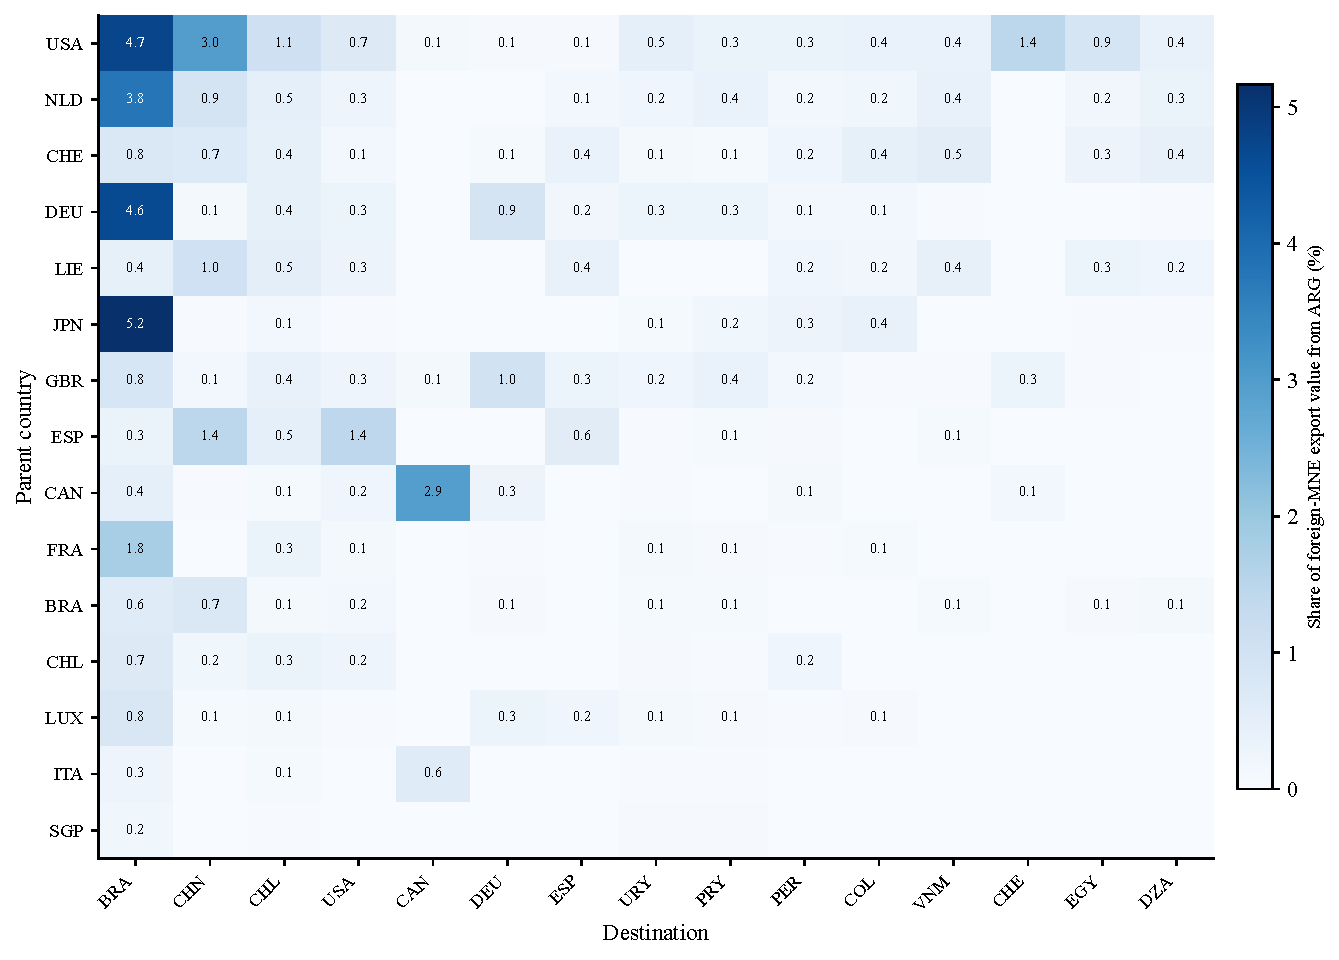
\includegraphics[width=1.0\textwidth,height=0.8\textheight,keepaspectratio]{figures/all/fig_wp1d_heatmap_country_cellpct_ARG.pdf}%
  \caption{Argentina: Foreign-Multinational Exports by Parent Country and Destination}%
  \label{fig:c_hm_ARG}%
  \par\vspace{2pt}%
  \parbox{0.92\textwidth}{\footnotesize %
  \textit{Notes:} Percent of the foreign-MNE export value of Argentina in each parent country and destination pair; fifteen largest parent countries and destinations.\\[3pt]%
  \textit{Source:} Authors' calculations based on customs data matched to Orbis and Dun \& Bradstreet.}%
  \end{figure}
% ---- Figure: Argentina: Share of Foreign-Multinational Exports Shipped to the Parent Country
\begin{figure}[H]\centering%
  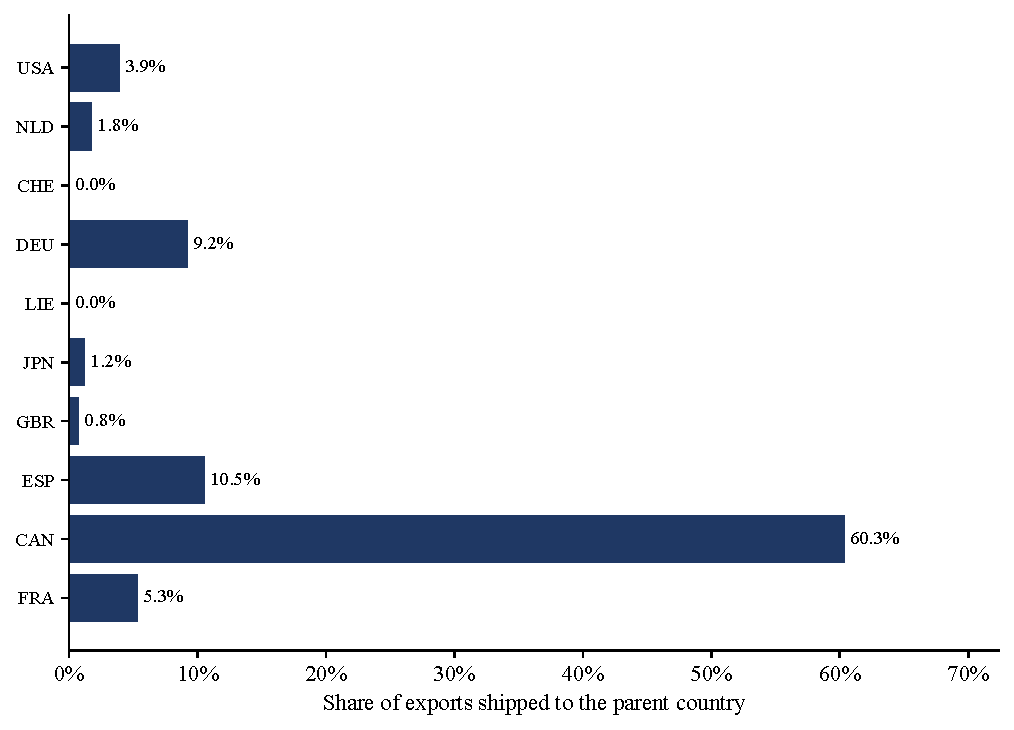
\includegraphics[width=0.85\textwidth,height=0.8\textheight,keepaspectratio]{figures/all/fig_wp1d_home_share_by_parent_ARG.pdf}%
  \caption{Argentina: Share of Foreign-Multinational Exports Shipped to the Parent Country}%
  \label{fig:c_home_ARG}%
  \par\vspace{2pt}%
  \parbox{0.92\textwidth}{\footnotesize %
  \textit{Notes:} Percent of each parent country's exports from Argentina shipped to that same country; ten largest parent countries.\\[3pt]%
  \textit{Source:} Authors' calculations based on customs data matched to Orbis and Dun \& Bradstreet.}%
  \end{figure}
% ---- Table: Argentina, Agriculture: Multinational Exports by Parent Region and Destination Region
\begin{table}[H]\centering\small%
  \caption{Argentina, Agriculture: Multinational Exports by Parent Region and Destination Region}%
  \label{tab:c_reg_ARG_agro}%
  \adjustbox{max width=\textwidth, max totalheight=0.8\textheight}{\begin{tabular}{lrrrrrrrr}
\toprule
ARG: parent region \ destination & Latin America & North America & Europe & Asia & Africa & Oceania & Rest of World & Total \\
\midrule
Latin America & 17.4 & 5.0 & 18.2 & 48.9 & 10.5 & 0.1 & 0.0 & 0.8 \\
North America & 26.1 & 2.3 & 7.7 & 46.9 & 17.0 & 0.1 & 0.0 & 3.0 \\
Europe & 24.4 & 1.6 & 18.7 & 42.8 & 12.1 & 0.4 & 0.0 & 9.2 \\
Asia & 13.3 & 20.1 & 24.6 & 31.7 & 9.4 & 0.9 & 0.0 & 0.4 \\
Africa & 41.4 & 7.9 & 25.8 & 6.8 & 18.1 & 0.0 & 0.0 & 0.1 \\
Oceania & 37.0 & 39.2 & 20.7 & 0.7 & 1.9 & 0.4 & 0.0 & 0.0 \\
Rest of World & 94.6 & 2.5 & 2.9 & 0.0 & 0.0 & 0.0 & 0.0 & 0.0 \\
Domestic MNEs & 19.4 & 2.2 & 18.3 & 43.8 & 14.4 & 2.0 & 0.0 & 3.7 \\
Local firms & 21.6 & 5.0 & 23.8 & 36.9 & 11.0 & 1.7 & 0.0 & 20.0 \\
\bottomrule
\end{tabular}
}%
  \par\vspace{3pt}%
  \begin{minipage}{0.95\textwidth}\footnotesize %
  \textit{Notes:} Percent of each group's agricultural exports from Argentina, by destination region (rows add to 100). Last column: the group's exports. Values are annual averages in US\$ billion.\\[3pt]%
  \textit{Source:} Authors' calculations based on customs data matched to Orbis and Dun \& Bradstreet.%
  \end{minipage}%
  \end{table}
% ---- Table: Argentina, Manufacturing: Multinational Exports by Parent Region and Destination Region
\begin{table}[H]\centering\small%
  \caption{Argentina, Manufacturing: Multinational Exports by Parent Region and Destination Region}%
  \label{tab:c_reg_ARG_manufacturing}%
  \adjustbox{max width=\textwidth, max totalheight=0.8\textheight}{\begin{tabular}{lrrrrrrrr}
\toprule
ARG: parent region \ destination & Latin America & North America & Europe & Asia & Africa & Oceania & Rest of World & Total \\
\midrule
Latin America & 76.8 & 6.5 & 3.3 & 12.4 & 0.9 & 0.1 & 0.0 & 1.1 \\
North America & 85.1 & 7.4 & 2.5 & 4.3 & 0.4 & 0.2 & 0.0 & 2.2 \\
Europe & 72.1 & 4.4 & 15.8 & 2.1 & 2.5 & 3.1 & 0.0 & 6.8 \\
Asia & 96.9 & 0.7 & 0.7 & 1.5 & 0.1 & 0.0 & 0.0 & 2.4 \\
Africa & 90.6 & 4.1 & 4.3 & 0.8 & 0.1 & 0.1 & 0.0 & 0.1 \\
Oceania & 13.2 & 2.6 & 22.3 & 61.5 & 0.3 & 0.1 & 0.0 & 0.1 \\
Rest of World & 96.5 & 0.0 & 3.5 & 0.0 & 0.0 & 0.0 & 0.0 & 0.0 \\
Domestic MNEs & 40.8 & 24.8 & 20.1 & 11.6 & 0.8 & 1.8 & 0.0 & 1.3 \\
Local firms & 56.3 & 16.3 & 13.4 & 11.2 & 2.5 & 0.3 & 0.0 & 7.3 \\
\bottomrule
\end{tabular}
}%
  \par\vspace{3pt}%
  \begin{minipage}{0.95\textwidth}\footnotesize %
  \textit{Notes:} Percent of each group's manufacturing exports from Argentina, by destination region (rows add to 100). Last column: the group's exports. Values are annual averages in US\$ billion.\\[3pt]%
  \textit{Source:} Authors' calculations based on customs data matched to Orbis and Dun \& Bradstreet.%
  \end{minipage}%
  \end{table}
% ---- Table: Argentina, Mining and Fuels: Multinational Exports by Parent Region and Destination Region
\begin{table}[H]\centering\small%
  \caption{Argentina, Mining and Fuels: Multinational Exports by Parent Region and Destination Region}%
  \label{tab:c_reg_ARG_mining}%
  \adjustbox{max width=\textwidth, max totalheight=0.8\textheight}{\begin{tabular}{lrrrrrrrr}
\toprule
ARG: parent region \ destination & Latin America & North America & Europe & Asia & Africa & Oceania & Rest of World & Total \\
\midrule
Latin America & 52.7 & 29.2 & 6.4 & 10.7 & 0.0 & 0.0 & 1.0 & 0.2 \\
North America & 2.0 & 57.8 & 36.6 & 3.5 & 0.0 & 0.0 & 0.0 & 1.7 \\
Europe & 25.7 & 25.8 & 21.7 & 26.0 & 0.7 & 0.1 & 0.0 & 2.9 \\
Asia & 5.0 & 85.7 & 7.3 & 0.3 & 0.1 & 1.7 & 0.0 & 0.1 \\
Africa & 93.1 & 0.0 & 6.9 & 0.0 & 0.0 & 0.0 & 0.0 & 0.0 \\
Oceania & 84.5 & 7.2 & 0.8 & 0.8 & 4.8 & 2.0 & 0.0 & 0.0 \\
Domestic MNEs & 80.7 & 3.6 & 11.6 & 3.6 & 0.5 & 0.0 & 0.0 & 0.0 \\
Local firms & 53.6 & 12.4 & 28.5 & 3.3 & 1.9 & 0.4 & 0.0 & 1.6 \\
\bottomrule
\end{tabular}
}%
  \par\vspace{3pt}%
  \begin{minipage}{0.95\textwidth}\footnotesize %
  \textit{Notes:} Percent of each group's mining and fuels exports from Argentina, by destination region (rows add to 100). Last column: the group's exports. Values are annual averages in US\$ billion.\\[3pt]%
  \textit{Source:} Authors' calculations based on customs data matched to Orbis and Dun \& Bradstreet.%
  \end{minipage}%
  \end{table}

\subsection{Products}
% ---- Table: Argentina: Fifteen Largest Export Products
\begin{table}[H]\centering\footnotesize%
  \caption{Argentina: Fifteen Largest Export Products}%
  \label{tab:c_hs6_ARG}%
  \adjustbox{max width=\textwidth, max totalheight=0.8\textheight}{\begin{tabular}{@{}l p{6.4cm} r r r r l@{}}
\toprule
HS6 & Description & US\$bn/yr & Foreign (\%) & Domestic (\%) & Local (\%) & Leading parent \\
\midrule
230400 & Oil-cake and other solid residues, whether/\allowbreak{}not ground/\allowbreak{}in pellets, from extraction of soyabean ... & 9.8 & 30 & 14 & 56 & CHE (0.44) \\
100590 & Maize (corn), other than seed & 4.3 & 51 & 7 & 41 & USA (0.36) \\
150710 & Soya bean oil, crude, whether/\allowbreak{}not degummed, not chemically modified & 3.8 & 26 & 15 & 59 & CHE (0.39) \\
870421 & Motor vehicles for the transportof goods (excl. of 8704.10), with C-I internal combustion pist... & 3.2 & 85 & 0 & 15 & DEU (0.50) \\
120100 & Soya beans, whether/\allowbreak{}not broken & 3.1 & 59 & 7 & 34 & USA (0.48) \\
710812 & Gold (incl. gold plated with platinum), in unwrought forms (excl. powder) & 2.1 & 79 & 0 & 21 & CAN (0.59) \\
100190 & Wheat other than durum wheat; meslin & 1.6 & 51 & 5 & 44 & LIE (0.25) \\
270900 & Petroleum oils and oils obt. from bituminous mins., crude & 1.4 & 92 & 0 & 8 & ESP (0.77) \\
382490 & Chemical productsandpreparations of the chemical/\allowbreak{}allied industries (including those consisting... & 1.2 & 35 & 15 & 50 & LIE (0.64) \\
870323 & Vehicles (excl. of 87.02 and 8703.10) principally designed for the transportof persons, with s... & 1.0 & 66 & 0 & 34 & NLD (0.43) \\
870322 & Vehicles (excl. of 87.02 and 8703.10) principally designed for the transportof persons, with s... & 0.8 & 100 & 0 & 0 & USA (0.59) \\
030613 & Shrimps and prawns, whether/\allowbreak{}not in shell, frozen & 0.7 & 66 & 9 & 24 & ESP (0.57) \\
220421 & Wine other than sparkling wine of fresh grapes, incl. fortified; grape must with fermentation ... & 0.7 & 22 & 2 & 76 & AUT (0.17) \\
260300 & Copper ores and concentrates & 0.7 & 100 & 0 & 0 & GBR (1.00) \\
020230 & Meat of bovine animals, frozen, boneless & 0.7 & 20 & 8 & 72 & BRA (0.64) \\
\bottomrule
\end{tabular}
}%
  \par\vspace{3pt}%
  \begin{minipage}{0.95\textwidth}\footnotesize %
  \textit{Notes:} Fifteen largest HS6 products exported by Argentina. Foreign, domestic and local: percent of the product's export value. Leading parent: largest parent country and its share of the product's foreign-MNE exports. Values are annual averages in US\$ billion.\\[3pt]%
  \textit{Source:} Authors' calculations based on customs data matched to Orbis and Dun \& Bradstreet.%
  \end{minipage}%
  \end{table}
% ---- Table: Argentina, Agriculture: Fifteen Largest Export Products
\begin{table}[H]\centering\footnotesize%
  \caption{Argentina, Agriculture: Fifteen Largest Export Products}%
  \label{tab:c_hs6_ARG_agro}%
  \adjustbox{max width=\textwidth, max totalheight=0.8\textheight}{\begin{tabular}{@{}l p{6.4cm} r r r r l@{}}
\toprule
HS6 & Description & US\$bn/yr & Foreign (\%) & Domestic (\%) & Local (\%) & Leading parent \\
\midrule
230400 & Oil-cake and other solid residues, whether/\allowbreak{}not ground/\allowbreak{}in pellets, from extraction of soyabean ... & 9.8 & 30 & 14 & 56 & CHE (0.44) \\
100590 & Maize (corn), other than seed & 4.3 & 51 & 7 & 41 & USA (0.36) \\
150710 & Soya bean oil, crude, whether/\allowbreak{}not degummed, not chemically modified & 3.8 & 26 & 15 & 59 & CHE (0.39) \\
120100 & Soya beans, whether/\allowbreak{}not broken & 3.1 & 59 & 7 & 34 & USA (0.48) \\
100190 & Wheat other than durum wheat; meslin & 1.6 & 51 & 5 & 44 & LIE (0.25) \\
030613 & Shrimps and prawns, whether/\allowbreak{}not in shell, frozen & 0.7 & 66 & 9 & 24 & ESP (0.57) \\
220421 & Wine other than sparkling wine of fresh grapes, incl. fortified; grape must with fermentation ... & 0.7 & 22 & 2 & 76 & AUT (0.17) \\
020230 & Meat of bovine animals, frozen, boneless & 0.7 & 20 & 8 & 72 & BRA (0.64) \\
020130 & Meat of bovine animals, fresh/\allowbreak{}chilled, boneless & 0.7 & 18 & 17 & 65 & BRA (0.82) \\
100300 & Barley & 0.5 & 55 & 4 & 42 & USA (0.37) \\
151211 & Sunflower seed/\allowbreak{}safflower oil, crude & 0.5 & 19 & 2 & 79 & NLD (0.70) \\
040221 & Milk in powder/\allowbreak{}granules/\allowbreak{}other solid form, unsweetened, fat content by weight >1.5\% & 0.5 & 32 & 32 & 36 & NLD (0.42) \\
200811 & Ground-nuts, prepared/\allowbreak{}preserved, whether/\allowbreak{}not containing added/\allowbreak{}sugar/\allowbreak{}other sweetening matter/\allowbreak{}sp... & 0.4 & 14 & 5 & 81 & SGP (0.45) \\
120190 & Soya beans, whether/\allowbreak{}not broken [HS 2007 line 120100] & 0.4 & 69 & 0 & 31 & USA (0.50) \\
080820 & Pears and quinces, fresh & 0.3 & 28 & 2 & 71 & BEL (0.42) \\
\bottomrule
\end{tabular}
}%
  \par\vspace{3pt}%
  \begin{minipage}{0.95\textwidth}\footnotesize %
  \textit{Notes:} Fifteen largest agricultural HS6 products exported by Argentina. Foreign, domestic and local: percent of the product's export value. Leading parent: largest parent country and its share of the product's foreign-MNE exports. Values are annual averages in US\$ billion.\\[3pt]%
  \textit{Source:} Authors' calculations based on customs data matched to Orbis and Dun \& Bradstreet.%
  \end{minipage}%
  \end{table}
% ---- Table: Argentina, Manufacturing: Fifteen Largest Export Products
\begin{table}[H]\centering\footnotesize%
  \caption{Argentina, Manufacturing: Fifteen Largest Export Products}%
  \label{tab:c_hs6_ARG_manufacturing}%
  \adjustbox{max width=\textwidth, max totalheight=0.8\textheight}{\begin{tabular}{@{}l p{6.4cm} r r r r l@{}}
\toprule
HS6 & Description & US\$bn/yr & Foreign (\%) & Domestic (\%) & Local (\%) & Leading parent \\
\midrule
870421 & Motor vehicles for the transportof goods (excl. of 8704.10), with C-I internal combustion pist... & 3.2 & 85 & 0 & 15 & DEU (0.50) \\
382490 & Chemical productsandpreparations of the chemical/\allowbreak{}allied industries (including those consisting... & 1.2 & 35 & 15 & 50 & LIE (0.64) \\
870323 & Vehicles (excl. of 87.02 and 8703.10) principally designed for the transportof persons, with s... & 1.0 & 66 & 0 & 34 & NLD (0.43) \\
870322 & Vehicles (excl. of 87.02 and 8703.10) principally designed for the transportof persons, with s... & 0.8 & 100 & 0 & 0 & USA (0.59) \\
880240 & Aeroplanes and other aircraft, of an unladen weight >15000kg & 0.6 & 41 & 52 & 7 & CHL (0.99) \\
870840 & Gear boxes and parts thereof, of the motor vehicles of headings 87.01 to 87.05. & 0.6 & 99 & 1 & 1 & DEU (0.88) \\
870321 & Vehicles (excl. of 87.02 and 8703.10) principally designed for the transportof persons, with s... & 0.5 & 100 & 0 & 0 & NLD (0.50) \\
730429 & Other casing, tubing, of a kind used in drilling for oil/\allowbreak{}gas (excld. of 7304.22/\allowbreak{}23/\allowbreak{}24), other ... & 0.5 & 0 & 0 & 100 & NLD (0.39) \\
410441 & Tanned/\allowbreak{}crust hides and skins of bovine (incl. buffalo)/\allowbreak{}equine animals, without hair on, in the... & 0.4 & 39 & 24 & 37 & BGR (0.45) \\
870431 & Motor vehicles for the transportof goods (excl. of 8704.10), with spark-ignition internal comb... & 0.4 & 47 & 0 & 53 & JPN (0.54) \\
300490 & Medicaments (excluding goods of heading 30.02/\allowbreak{}30.05/\allowbreak{}30.06/\allowbreak{}3004.10-3004.50) consisting of mixed... & 0.4 & 58 & 4 & 38 & USA (0.38) \\
870333 & Vehicles principally designed for the transportof persons (excl. of 87.02 and 8703.10-8703.24)... & 0.4 & 100 & 0 & 0 & JPN (1.00) \\
760110 & Aluminium, not alloyed, unwrought & 0.4 & 0 & 0 & 100 & -- \\
330720 & Personal deodorants and antiperspirants & 0.3 & 79 & 2 & 19 & GBR (0.94) \\
760120 & Aluminium alloys, unwrought & 0.2 & 0 & 0 & 100 & DEU (1.00) \\
\bottomrule
\end{tabular}
}%
  \par\vspace{3pt}%
  \begin{minipage}{0.95\textwidth}\footnotesize %
  \textit{Notes:} Fifteen largest manufacturing HS6 products exported by Argentina. Foreign, domestic and local: percent of the product's export value. Leading parent: largest parent country and its share of the product's foreign-MNE exports. Values are annual averages in US\$ billion.\\[3pt]%
  \textit{Source:} Authors' calculations based on customs data matched to Orbis and Dun \& Bradstreet.%
  \end{minipage}%
  \end{table}
% ---- Table: Argentina, Mining and Fuels: Fifteen Largest Export Products
\begin{table}[H]\centering\footnotesize%
  \caption{Argentina, Mining and Fuels: Fifteen Largest Export Products}%
  \label{tab:c_hs6_ARG_mining}%
  \adjustbox{max width=\textwidth, max totalheight=0.8\textheight}{\begin{tabular}{@{}l p{6.4cm} r r r r l@{}}
\toprule
HS6 & Description & US\$bn/yr & Foreign (\%) & Domestic (\%) & Local (\%) & Leading parent \\
\midrule
710812 & Gold (incl. gold plated with platinum), in unwrought forms (excl. powder) & 2.1 & 79 & 0 & 21 & CAN (0.59) \\
270900 & Petroleum oils and oils obt. from bituminous mins., crude & 1.4 & 92 & 0 & 8 & ESP (0.77) \\
260300 & Copper ores and concentrates & 0.7 & 100 & 0 & 0 & GBR (1.00) \\
271011 & Light petroleum oils and preparations & 0.6 & 38 & 0 & 62 & GBR (0.41) \\
710691 & Silver (incl. silver plated with gold/\allowbreak{}platinum), unwrought & 0.3 & 88 & 0 & 12 & CAN (0.47) \\
261610 & Silver ores and concentrates & 0.3 & 99 & 0 & 1 & GBR (0.51) \\
271112 & Propane, liquefied & 0.2 & 39 & 0 & 61 & FRA (0.79) \\
271019 & Petroleum oils and oils obtained from bituminous minerals (other than crude) and preparations ... & 0.2 & 59 & 2 & 39 & BRA (0.64) \\
271113 & Butanes, liquefied & 0.2 & 31 & 0 & 69 & FRA (0.87) \\
271119 & Petroleum gases other than natural gas/\allowbreak{}propane/\allowbreak{}butanes/\allowbreak{}ethylene, propylene, butylene and butad... & 0.1 & 55 & 0 & 45 & FRA (0.38) \\
271121 & Natural gas, in gaseous state & 0.1 & 70 & 0 & 30 & DEU (0.30) \\
271012 & Light petroleum oils and preparations [HS2012 code] & 0.0 & 50 & 0 & 50 & ESP (0.48) \\
260700 & Lead ores and concentrates & 0.0 & 0 & 0 & 100 & -- \\
271312 & Petroleum coke, calcined & 0.0 & 0 & 0 & 100 & CYP (0.75) \\
252210 & Quicklime & 0.0 & 18 & 0 & 82 & MEX (0.87) \\
\bottomrule
\end{tabular}
}%
  \par\vspace{3pt}%
  \begin{minipage}{0.95\textwidth}\footnotesize %
  \textit{Notes:} Fifteen largest mining and fuels HS6 products exported by Argentina. Foreign, domestic and local: percent of the product's export value. Leading parent: largest parent country and its share of the product's foreign-MNE exports. Values are annual averages in US\$ billion.\\[3pt]%
  \textit{Source:} Authors' calculations based on customs data matched to Orbis and Dun \& Bradstreet.%
  \end{minipage}%
  \end{table}

\section{Chile}\label{sec:c_CHL}

\subsection{Parents and Destinations}
% ---- Table: Chile: Multinational Exports by Parent Region and Destination Region
\begin{table}[H]\centering\small%
  \caption{Chile: Multinational Exports by Parent Region and Destination Region}%
  \label{tab:c_reg_CHL}%
  \adjustbox{max width=\textwidth, max totalheight=0.8\textheight}{\begin{tabular}{lrrrrrrrr}
\toprule
CHL: parent region \ destination & Latin America & North America & Europe & Asia & Africa & Oceania & Rest of World & Total \\
\midrule
Latin America & 18.4 & 8.8 & 10.3 & 61.7 & 0.3 & 0.5 & 0.0 & 1.2 \\
North America & 19.4 & 17.8 & 27.6 & 35.0 & 0.2 & 0.1 & 0.0 & 3.3 \\
Europe & 9.1 & 8.9 & 9.1 & 71.1 & 0.2 & 1.7 & 0.0 & 10.3 \\
Asia & 12.9 & 17.7 & 10.1 & 58.7 & 0.1 & 0.6 & 0.0 & 0.5 \\
Africa & 47.0 & 8.6 & 22.2 & 20.2 & 1.5 & 0.2 & 0.2 & 0.0 \\
Oceania & 6.3 & 85.2 & 2.7 & 4.8 & 0.1 & 0.9 & 0.0 & 0.0 \\
Rest of World & 76.6 & 0.0 & 5.1 & 18.2 & 0.0 & 0.0 & 0.0 & 0.0 \\
Domestic MNEs & 21.9 & 16.1 & 14.7 & 45.4 & 0.8 & 1.0 & 0.0 & 4.6 \\
Local firms & 15.5 & 18.8 & 20.4 & 44.3 & 0.6 & 0.5 & 0.0 & 13.2 \\
\bottomrule
\end{tabular}
}%
  \par\vspace{3pt}%
  \begin{minipage}{0.95\textwidth}\footnotesize %
  \textit{Notes:} Percent of each group's exports from Chile, by destination region (rows add to 100). Last column: the group's exports. Values are annual averages in US\$ billion.\\[3pt]%
  \textit{Source:} Authors' calculations based on customs data matched to Orbis and Dun \& Bradstreet.%
  \end{minipage}%
  \end{table}
% ---- Figure: Chile: Foreign-Multinational Exports by Parent Country and Destination
\begin{figure}[H]\centering%
  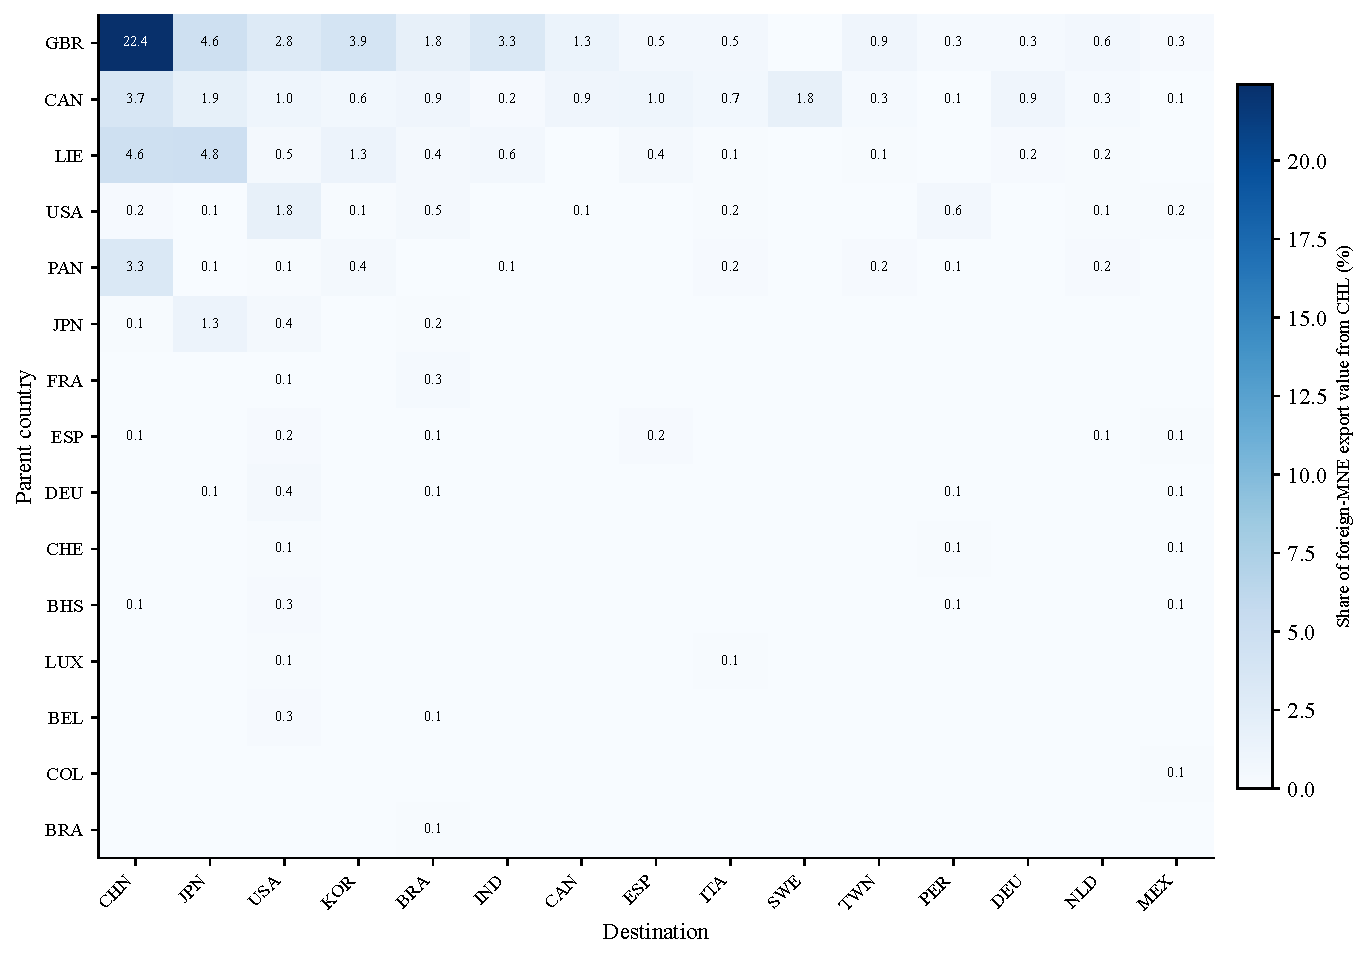
\includegraphics[width=1.0\textwidth,height=0.8\textheight,keepaspectratio]{figures/all/fig_wp1d_heatmap_country_cellpct_CHL.pdf}%
  \caption{Chile: Foreign-Multinational Exports by Parent Country and Destination}%
  \label{fig:c_hm_CHL}%
  \par\vspace{2pt}%
  \parbox{0.92\textwidth}{\footnotesize %
  \textit{Notes:} Percent of the foreign-MNE export value of Chile in each parent country and destination pair; fifteen largest parent countries and destinations.\\[3pt]%
  \textit{Source:} Authors' calculations based on customs data matched to Orbis and Dun \& Bradstreet.}%
  \end{figure}
% ---- Figure: Chile: Share of Foreign-Multinational Exports Shipped to the Parent Country
\begin{figure}[H]\centering%
  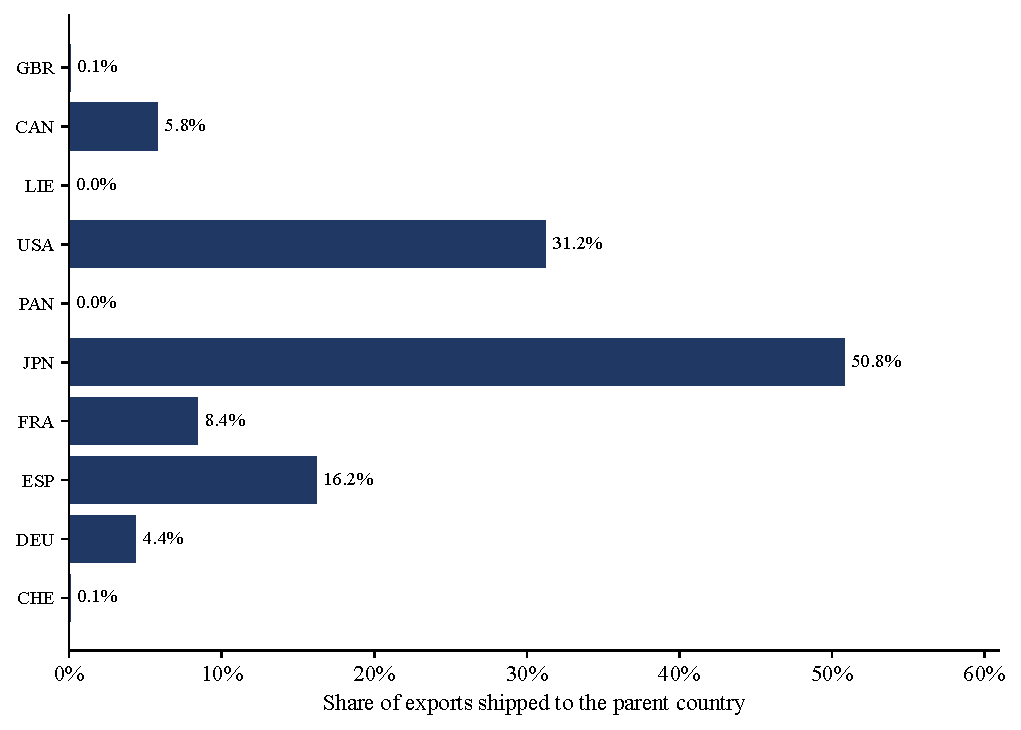
\includegraphics[width=0.85\textwidth,height=0.8\textheight,keepaspectratio]{figures/all/fig_wp1d_home_share_by_parent_CHL.pdf}%
  \caption{Chile: Share of Foreign-Multinational Exports Shipped to the Parent Country}%
  \label{fig:c_home_CHL}%
  \par\vspace{2pt}%
  \parbox{0.92\textwidth}{\footnotesize %
  \textit{Notes:} Percent of each parent country's exports from Chile shipped to that same country; ten largest parent countries.\\[3pt]%
  \textit{Source:} Authors' calculations based on customs data matched to Orbis and Dun \& Bradstreet.}%
  \end{figure}
% ---- Table: Chile, Agriculture: Multinational Exports by Parent Region and Destination Region
\begin{table}[H]\centering\small%
  \caption{Chile, Agriculture: Multinational Exports by Parent Region and Destination Region}%
  \label{tab:c_reg_CHL_agro}%
  \adjustbox{max width=\textwidth, max totalheight=0.8\textheight}{\begin{tabular}{lrrrrrrrr}
\toprule
CHL: parent region \ destination & Latin America & North America & Europe & Asia & Africa & Oceania & Rest of World & Total \\
\midrule
Latin America & 40.3 & 18.2 & 14.4 & 25.8 & 1.2 & 0.2 & 0.0 & 0.1 \\
North America & 34.3 & 26.0 & 16.1 & 22.7 & 0.5 & 0.3 & 0.0 & 0.5 \\
Europe & 30.5 & 23.6 & 25.8 & 15.0 & 1.7 & 3.3 & 0.0 & 0.7 \\
Asia & 10.2 & 20.4 & 11.3 & 57.6 & 0.0 & 0.4 & 0.0 & 0.4 \\
Africa & 9.1 & 18.9 & 29.4 & 40.3 & 2.3 & 0.1 & 0.0 & 0.0 \\
Oceania & 2.9 & 26.6 & 9.1 & 59.3 & 0.6 & 1.5 & 0.0 & 0.0 \\
Rest of World & 0.0 & 0.0 & 0.0 & 100.0 & 0.0 & 0.0 & 0.0 & 0.0 \\
Domestic MNEs & 18.6 & 26.4 & 18.0 & 36.4 & 0.3 & 0.2 & 0.0 & 1.4 \\
Local firms & 17.9 & 27.4 & 24.9 & 28.3 & 1.1 & 0.4 & 0.0 & 3.9 \\
\bottomrule
\end{tabular}
}%
  \par\vspace{3pt}%
  \begin{minipage}{0.95\textwidth}\footnotesize %
  \textit{Notes:} Percent of each group's agricultural exports from Chile, by destination region (rows add to 100). Last column: the group's exports. Values are annual averages in US\$ billion.\\[3pt]%
  \textit{Source:} Authors' calculations based on customs data matched to Orbis and Dun \& Bradstreet.%
  \end{minipage}%
  \end{table}
% ---- Table: Chile, Manufacturing: Multinational Exports by Parent Region and Destination Region
\begin{table}[H]\centering\small%
  \caption{Chile, Manufacturing: Multinational Exports by Parent Region and Destination Region}%
  \label{tab:c_reg_CHL_manufacturing}%
  \adjustbox{max width=\textwidth, max totalheight=0.8\textheight}{\begin{tabular}{lrrrrrrrr}
\toprule
CHL: parent region \ destination & Latin America & North America & Europe & Asia & Africa & Oceania & Rest of World & Total \\
\midrule
Latin America & 15.4 & 7.4 & 9.5 & 67.0 & 0.2 & 0.6 & 0.0 & 1.0 \\
North America & 28.2 & 19.6 & 15.8 & 36.1 & 0.2 & 0.2 & 0.0 & 1.4 \\
Europe & 13.7 & 18.4 & 10.5 & 53.2 & 0.1 & 4.1 & 0.0 & 3.6 \\
Asia & 23.6 & 6.3 & 4.4 & 64.2 & 0.2 & 1.3 & 0.0 & 0.1 \\
Africa & 25.2 & 4.2 & 39.4 & 28.3 & 2.3 & 0.6 & 0.0 & 0.0 \\
Oceania & 48.9 & 22.6 & 19.1 & 1.5 & 0.3 & 7.5 & 0.0 & 0.0 \\
Rest of World & 93.7 & 0.0 & 6.3 & 0.0 & 0.0 & 0.0 & 0.0 & 0.0 \\
Domestic MNEs & 24.9 & 15.3 & 16.2 & 40.7 & 1.0 & 1.7 & 0.0 & 2.3 \\
Local firms & 14.5 & 16.9 & 16.6 & 51.0 & 0.4 & 0.6 & 0.0 & 7.3 \\
\bottomrule
\end{tabular}
}%
  \par\vspace{3pt}%
  \begin{minipage}{0.95\textwidth}\footnotesize %
  \textit{Notes:} Percent of each group's manufacturing exports from Chile, by destination region (rows add to 100). Last column: the group's exports. Values are annual averages in US\$ billion.\\[3pt]%
  \textit{Source:} Authors' calculations based on customs data matched to Orbis and Dun \& Bradstreet.%
  \end{minipage}%
  \end{table}
% ---- Table: Chile, Mining and Fuels: Multinational Exports by Parent Region and Destination Region
\begin{table}[H]\centering\small%
  \caption{Chile, Mining and Fuels: Multinational Exports by Parent Region and Destination Region}%
  \label{tab:c_reg_CHL_mining}%
  \adjustbox{max width=\textwidth, max totalheight=0.8\textheight}{\begin{tabular}{lrrrrrrrr}
\toprule
CHL: parent region \ destination & Latin America & North America & Europe & Asia & Africa & Oceania & Rest of World & Total \\
\midrule
Latin America & 85.5 & 0.3 & 0.0 & 14.0 & 0.2 & 0.0 & 0.0 & 0.0 \\
North America & 1.6 & 11.5 & 46.4 & 40.5 & 0.0 & 0.0 & 0.0 & 1.3 \\
Europe & 3.6 & 1.1 & 6.0 & 89.2 & 0.1 & 0.1 & 0.0 & 6.0 \\
Asia & 2.5 & 25.6 & 34.5 & 37.4 & 0.0 & 0.0 & 0.0 & 0.0 \\
Africa & 1.4 & 98.2 & 0.4 & 0.0 & 0.0 & 0.0 & 0.0 & 0.0 \\
Oceania & 0.0 & 99.9 & 0.1 & 0.0 & 0.0 & 0.0 & 0.0 & 0.0 \\
Domestic MNEs & 6.1 & 2.1 & 6.4 & 83.9 & 1.2 & 0.3 & 0.0 & 0.8 \\
Local firms & 12.3 & 8.5 & 25.3 & 53.3 & 0.4 & 0.2 & 0.0 & 1.9 \\
\bottomrule
\end{tabular}
}%
  \par\vspace{3pt}%
  \begin{minipage}{0.95\textwidth}\footnotesize %
  \textit{Notes:} Percent of each group's mining and fuels exports from Chile, by destination region (rows add to 100). Last column: the group's exports. Values are annual averages in US\$ billion.\\[3pt]%
  \textit{Source:} Authors' calculations based on customs data matched to Orbis and Dun \& Bradstreet.%
  \end{minipage}%
  \end{table}
% ---- Table: Chile, Other Goods: Multinational Exports by Parent Region and Destination Region
\begin{table}[H]\centering\small%
  \caption{Chile, Other Goods: Multinational Exports by Parent Region and Destination Region}%
  \label{tab:c_reg_CHL_rest}%
  \adjustbox{max width=\textwidth, max totalheight=0.8\textheight}{\begin{tabular}{lrrrrrrrr}
\toprule
CHL: parent region \ destination & Latin America & North America & Europe & Asia & Africa & Oceania & Rest of World & Total \\
\midrule
Latin America & 33.0 & 22.3 & 40.0 & 3.8 & 0.1 & 0.2 & 0.7 & 0.0 \\
North America & 52.1 & 38.7 & 7.8 & 1.3 & 0.0 & 0.1 & 0.0 & 0.1 \\
Europe & 30.2 & 37.1 & 30.2 & 2.0 & 0.2 & 0.4 & 0.0 & 0.1 \\
Asia & 24.1 & 19.2 & 14.2 & 42.4 & 0.0 & 0.1 & 0.0 & 0.0 \\
Africa & 82.8 & 2.7 & 10.8 & 2.7 & 0.7 & 0.0 & 0.4 & 0.0 \\
Oceania & 78.6 & 7.2 & 0.3 & 12.3 & 0.0 & 1.6 & 0.0 & 0.0 \\
Rest of World & 5.0 & 0.0 & 0.0 & 95.0 & 0.0 & 0.0 & 0.0 & 0.0 \\
Domestic MNEs & 92.6 & 4.0 & 3.0 & 0.4 & 0.0 & 0.0 & 0.0 & 0.1 \\
Local firms & 50.7 & 17.5 & 27.3 & 4.0 & 0.2 & 0.2 & 0.0 & 0.1 \\
\bottomrule
\end{tabular}
}%
  \par\vspace{3pt}%
  \begin{minipage}{0.95\textwidth}\footnotesize %
  \textit{Notes:} Percent of each group's exports from Chile, by destination region (rows add to 100). Last column: the group's exports. Values are annual averages in US\$ billion.\\[3pt]%
  \textit{Source:} Authors' calculations based on customs data matched to Orbis and Dun \& Bradstreet.%
  \end{minipage}%
  \end{table}

\subsection{Products}
% ---- Table: Chile: Fifteen Largest Export Products
\begin{table}[H]\centering\footnotesize%
  \caption{Chile: Fifteen Largest Export Products}%
  \label{tab:c_hs6_CHL}%
  \adjustbox{max width=\textwidth, max totalheight=0.8\textheight}{\begin{tabular}{@{}l p{6.4cm} r r r r l@{}}
\toprule
HS6 & Description & US\$bn/yr & Foreign (\%) & Domestic (\%) & Local (\%) & Leading parent \\
\midrule
740311 & Cathodes and sections of cathodes, of refined copper, unwrought & 8.5 & 36 & 3 & 61 & GBR (0.62) \\
260300 & Copper ores and concentrates & 7.8 & 86 & 2 & 12 & GBR (0.62) \\
740200 & Unrefined copper; copper anodes for electrolytic refining & 1.2 & 80 & 1 & 19 & GBR (1.00) \\
220421 & Wine other than sparkling wine of fresh grapes, incl. fortified; grape must with fermentation ... & 0.7 & 22 & 17 & 61 & FRA (0.40) \\
470321 & Chemical wood pulp, soda/\allowbreak{}sulphate, other than dissolving grades, semi-bleached/\allowbreak{}bleached, conif... & 0.6 & 66 & 34 & 0 & PAN (1.00) \\
470329 & Chemical wood pulp, soda/\allowbreak{}sulphate, other than dissolving grades, semi-bleached/\allowbreak{}bleached, non-c... & 0.6 & 46 & 54 & 0 & PAN (1.00) \\
080610 & Grapes, fresh & 0.5 & 22 & 14 & 64 & USA (0.39) \\
710812 & Gold (incl. gold plated with platinum), in unwrought forms (excl. powder) & 0.5 & 66 & 1 & 34 & CAN (0.92) \\
261310 & Molybdenum ores and concentrates, roasted & 0.5 & 25 & 0 & 75 & GBR (0.57) \\
260111 & Iron ores and concentrates (excl. roasted iron pyrites), non-agglomerated & 0.5 & 4 & 95 & 2 & CAN (0.66) \\
283691 & Lithium carbonates & 0.4 & 0 & 75 & 25 & -- \\
030441 & Fish filletsandother fish meat (excl. of 0304.11-0304.12, whether/\allowbreak{}not minced), fresh/\allowbreak{}chilled [... & 0.4 & 20 & 24 & 56 & JPN (0.50) \\
002599 & National /\allowbreak{} special customs line (no HS description) & 0.4 & 48 & 31 & 21 & USA (0.39) \\
080810 & Apples, fresh & 0.3 & 26 & 17 & 57 & USA (0.45) \\
080929 & Cherries, fresh [HS 2007 line 080920] & 0.3 & 22 & 17 & 61 & USA (0.30) \\
\bottomrule
\end{tabular}
}%
  \par\vspace{3pt}%
  \begin{minipage}{0.95\textwidth}\footnotesize %
  \textit{Notes:} Fifteen largest HS6 products exported by Chile. Foreign, domestic and local: percent of the product's export value. Leading parent: largest parent country and its share of the product's foreign-MNE exports. Values are annual averages in US\$ billion.\\[3pt]%
  \textit{Source:} Authors' calculations based on customs data matched to Orbis and Dun \& Bradstreet.%
  \end{minipage}%
  \end{table}
% ---- Table: Chile, Agriculture: Fifteen Largest Export Products
\begin{table}[H]\centering\footnotesize%
  \caption{Chile, Agriculture: Fifteen Largest Export Products}%
  \label{tab:c_hs6_CHL_agro}%
  \adjustbox{max width=\textwidth, max totalheight=0.8\textheight}{\begin{tabular}{@{}l p{6.4cm} r r r r l@{}}
\toprule
HS6 & Description & US\$bn/yr & Foreign (\%) & Domestic (\%) & Local (\%) & Leading parent \\
\midrule
220421 & Wine other than sparkling wine of fresh grapes, incl. fortified; grape must with fermentation ... & 0.70 & 22 & 17 & 61 & FRA (0.40) \\
080610 & Grapes, fresh & 0.53 & 22 & 14 & 64 & USA (0.39) \\
030441 & Fish filletsandother fish meat (excl. of 0304.11-0304.12, whether/\allowbreak{}not minced), fresh/\allowbreak{}chilled [... & 0.40 & 20 & 24 & 56 & JPN (0.50) \\
080810 & Apples, fresh & 0.29 & 26 & 17 & 57 & USA (0.45) \\
080929 & Cherries, fresh [HS 2007 line 080920] & 0.28 & 22 & 17 & 61 & USA (0.30) \\
030481 & Fish filletsandother fish meat (excl. of 0304.21-0304.92, whether/\allowbreak{}not minced), frozen fillets ... & 0.25 & 15 & 22 & 63 & JPN (0.38) \\
030214 & Pacific salmon/\allowbreak{}Atlantic salmon/\allowbreak{}Danube salmon [see list of conventions for species incld.], fre... & 0.25 & 21 & 21 & 58 & JPN (0.42) \\
030312 & Pacific salmon (Oncorhynchus gorbuscha/\allowbreak{}keta/\allowbreak{}tschawytscha/\allowbreak{}kisutch/\allowbreak{}masou/\allowbreak{}rhodurus), frozen (excl... & 0.23 & 23 & 27 & 50 & JPN (0.78) \\
230120 & Flours, meals and pellets of fish/\allowbreak{}of crustaceans, molluscs/\allowbreak{}other aquatic invertebrates & 0.20 & 18 & 12 & 70 & ALB (0.60) \\
030313 & Atlantic salmon (Salmo salar) and Danube salmon (Hucho hucho), frozen (excl. fillets/\allowbreak{}other fis... & 0.20 & 33 & 21 & 46 & JPN (0.42) \\
081040 & Cranberries, bilberries and other fruits of the genus Vaccinium, fresh & 0.19 & 23 & 23 & 54 & DEU (0.28) \\
020329 & Meat of swine (excl. carcasses/\allowbreak{}half-carcasses/\allowbreak{}hams/\allowbreak{}shoulders and cuts thereof ), froxen & 0.18 & 30 & 56 & 14 & JPN (1.00) \\
220429 & Wine other than sparkling wine of fresh grapes, incl. fortified; grape must with fermentation ... & 0.14 & 16 & 12 & 71 & CHN (0.51) \\
030499 & Fish filletsandother fish meat (excl. of 0304.11-0304.29, whether/\allowbreak{}not minced),n.e.s. & 0.14 & 45 & 18 & 37 & USA (0.50) \\
020714 & Cuts and edible offal of species Gallus domesticus, frozen & 0.13 & 0 & 62 & 38 & -- \\
\bottomrule
\end{tabular}
}%
  \par\vspace{3pt}%
  \begin{minipage}{0.95\textwidth}\footnotesize %
  \textit{Notes:} Fifteen largest agricultural HS6 products exported by Chile. Foreign, domestic and local: percent of the product's export value. Leading parent: largest parent country and its share of the product's foreign-MNE exports. Values are annual averages in US\$ billion.\\[3pt]%
  \textit{Source:} Authors' calculations based on customs data matched to Orbis and Dun \& Bradstreet.%
  \end{minipage}%
  \end{table}
% ---- Table: Chile, Manufacturing: Fifteen Largest Export Products
\begin{table}[H]\centering\footnotesize%
  \caption{Chile, Manufacturing: Fifteen Largest Export Products}%
  \label{tab:c_hs6_CHL_manufacturing}%
  \adjustbox{max width=\textwidth, max totalheight=0.8\textheight}{\begin{tabular}{@{}l p{6.4cm} r r r r l@{}}
\toprule
HS6 & Description & US\$bn/yr & Foreign (\%) & Domestic (\%) & Local (\%) & Leading parent \\
\midrule
740311 & Cathodes and sections of cathodes, of refined copper, unwrought & 8.5 & 36 & 3 & 61 & GBR (0.62) \\
740200 & Unrefined copper; copper anodes for electrolytic refining & 1.2 & 80 & 1 & 19 & GBR (1.00) \\
470321 & Chemical wood pulp, soda/\allowbreak{}sulphate, other than dissolving grades, semi-bleached/\allowbreak{}bleached, conif... & 0.6 & 66 & 34 & 0 & PAN (1.00) \\
470329 & Chemical wood pulp, soda/\allowbreak{}sulphate, other than dissolving grades, semi-bleached/\allowbreak{}bleached, non-c... & 0.6 & 46 & 54 & 0 & PAN (1.00) \\
283691 & Lithium carbonates & 0.4 & 0 & 75 & 25 & -- \\
280120 & Iodine & 0.3 & 8 & 17 & 76 & CAN (1.00) \\
440710 & Wood sawn/\allowbreak{}chipped length wise, sliced/\allowbreak{}peeled, whether/\allowbreak{}not planed, sanded/\allowbreak{}end-jointed, of a thi... & 0.2 & 10 & 32 & 59 & BHS (0.93) \\
440711 & Wood sawn/\allowbreak{}chipped length wise, sliced/\allowbreak{}peeled, whether/\allowbreak{}not planed, sanded/\allowbreak{}end-jointed, of a thi... & 0.2 & 9 & 73 & 18 & BHS (0.88) \\
441239 & Plywood, consisting solely of sheets of wood (other than bamboo,excl. of 4412.31 and4412.32), ... & 0.2 & 16 & 83 & 1 & USA (0.58) \\
740811 & Copper wire, of refined copper of which the maximum cross-sectional dim. exceeds 6mm & 0.2 & 90 & 0 & 10 & USA (0.61) \\
440122 & Wood, in chips/\allowbreak{}particles, non-coniferous & 0.2 & 44 & 26 & 30 & JPN (0.93) \\
481092 & Paper and paperboard(excl. of 4810.13-4810.39), coated on one/\allowbreak{}both sides with kaolin (China cl... & 0.2 & 0 & 100 & 0 & ITA (0.67) \\
310420 & Potassium chloride & 0.1 & 2 & 97 & 1 & DZA (0.85) \\
401110 & New pneumatic tyres, of rubber, of a kind used on motor cars (incl. station wagons and racing ... & 0.1 & 100 & 0 & 0 & USA (1.00) \\
740400 & Copper waste and scrap & 0.1 & 11 & 3 & 86 & GBR (0.90) \\
\bottomrule
\end{tabular}
}%
  \par\vspace{3pt}%
  \begin{minipage}{0.95\textwidth}\footnotesize %
  \textit{Notes:} Fifteen largest manufacturing HS6 products exported by Chile. Foreign, domestic and local: percent of the product's export value. Leading parent: largest parent country and its share of the product's foreign-MNE exports. Values are annual averages in US\$ billion.\\[3pt]%
  \textit{Source:} Authors' calculations based on customs data matched to Orbis and Dun \& Bradstreet.%
  \end{minipage}%
  \end{table}
% ---- Table: Chile, Mining and Fuels: Fifteen Largest Export Products
\begin{table}[H]\centering\footnotesize%
  \caption{Chile, Mining and Fuels: Fifteen Largest Export Products}%
  \label{tab:c_hs6_CHL_mining}%
  \adjustbox{max width=\textwidth, max totalheight=0.8\textheight}{\begin{tabular}{@{}l p{6.4cm} r r r r l@{}}
\toprule
HS6 & Description & US\$bn/yr & Foreign (\%) & Domestic (\%) & Local (\%) & Leading parent \\
\midrule
260300 & Copper ores and concentrates & 7.8 & 86 & 2 & 12 & GBR (0.62) \\
710812 & Gold (incl. gold plated with platinum), in unwrought forms (excl. powder) & 0.5 & 66 & 1 & 34 & CAN (0.92) \\
261310 & Molybdenum ores and concentrates, roasted & 0.5 & 25 & 0 & 75 & GBR (0.57) \\
260111 & Iron ores and concentrates (excl. roasted iron pyrites), non-agglomerated & 0.5 & 4 & 95 & 2 & CAN (0.66) \\
710691 & Silver (incl. silver plated with gold/\allowbreak{}platinum), unwrought & 0.2 & 62 & 0 & 38 & CAN (0.99) \\
261390 & Molybdenum ores and concentrates, other than roasted & 0.1 & 71 & 0 & 29 & LIE (0.83) \\
260112 & Iron ores and concentrates (excl. roasted iron pyrites), agglomerated & 0.1 & 8 & 92 & 0 & CHE (1.00) \\
262099 & Ash and residues (excl. from the manufacture of iron/\allowbreak{}steel), n.e.s. in Ch.26 & 0.1 & 0 & 0 & 100 & CAN (0.96) \\
271019 & Petroleum oils and oils obtained from bituminous minerals (other than crude) and preparations ... & 0.1 & 5 & 8 & 87 & DEU (0.59) \\
250100 & Salt (incl. table salt and denatured salt) and pure sodium chloride, whether/\allowbreak{}not in aqueous so... & 0.1 & 74 & 1 & 25 & BEL (1.00) \\
260800 & Zinc ores and concentrates & 0.0 & 14 & 18 & 67 & CAN (0.98) \\
271012 & Light petroleum oils and preparations [HS2012 code] & 0.0 & 0 & 12 & 88 & ESP (0.96) \\
271011 & Light petroleum oils and preparations & 0.0 & 0 & 1 & 99 & USA (0.54) \\
261610 & Silver ores and concentrates & 0.0 & 100 & 0 & 0 & CAN (1.00) \\
262030 & Ash and residues (excl. from the manufacture of iron/\allowbreak{}steel) containing mainly copper & 0.0 & 1 & 84 & 15 & DEU (1.00) \\
\bottomrule
\end{tabular}
}%
  \par\vspace{3pt}%
  \begin{minipage}{0.95\textwidth}\footnotesize %
  \textit{Notes:} Fifteen largest mining and fuels HS6 products exported by Chile. Foreign, domestic and local: percent of the product's export value. Leading parent: largest parent country and its share of the product's foreign-MNE exports. Values are annual averages in US\$ billion.\\[3pt]%
  \textit{Source:} Authors' calculations based on customs data matched to Orbis and Dun \& Bradstreet.%
  \end{minipage}%
  \end{table}
% ---- Table: Chile, Other Goods: Fifteen Largest Export Products
\begin{table}[H]\centering\footnotesize%
  \caption{Chile, Other Goods: Fifteen Largest Export Products}%
  \label{tab:c_hs6_CHL_rest}%
  \adjustbox{max width=\textwidth, max totalheight=0.8\textheight}{\begin{tabular}{@{}l p{6.4cm} r r r r l@{}}
\toprule
HS6 & Description & US\$bn/yr & Foreign (\%) & Domestic (\%) & Local (\%) & Leading parent \\
\midrule
002599 & National /\allowbreak{} special customs line (no HS description) & 0.36 & 48 & 31 & 21 & USA (0.39) \\
002500 & National /\allowbreak{} special customs line (no HS description) & 0.11 & 51 & 21 & 28 & USA (0.44) \\
002501 & National /\allowbreak{} special customs line (no HS description) & 0.01 & 67 & 5 & 28 & DEU (0.60) \\
000199 & National /\allowbreak{} special customs line (no HS description) & 0.00 & 100 & 0 & 0 & EGY (1.00) \\
001600 & National /\allowbreak{} special customs line (no HS description) & 0.00 & 12 & 0 & 88 & USA (0.99) \\
001989 & National /\allowbreak{} special customs line (no HS description) & 0.00 & 92 & 0 & 8 & GBR (0.97) \\
000000 & National /\allowbreak{} special customs line (no HS description) & 0.00 & 0 & 61 & 39 & -- \\
000905 & National /\allowbreak{} special customs line (no HS description) & 0.00 & 0 & 0 & 100 & -- \\
000500 & National /\allowbreak{} special customs line (no HS description) & 0.00 & 0 & 0 & 100 & -- \\
000904 & National /\allowbreak{} special customs line (no HS description) & 0.00 & 0 & 0 & 100 & -- \\
000901 & National /\allowbreak{} special customs line (no HS description) & 0.00 & 47 & 0 & 53 & GBR (1.00) \\
001400 & National /\allowbreak{} special customs line (no HS description) & 0.00 & 100 & 0 & 0 & -- \\
002102 & National /\allowbreak{} special customs line (no HS description) & 0.00 & 0 & 0 & 100 & -- \\
000802 & National /\allowbreak{} special customs line (no HS description) & 0.00 & 0 & 0 & 100 & -- \\
\bottomrule
\end{tabular}
}%
  \par\vspace{3pt}%
  \begin{minipage}{0.95\textwidth}\footnotesize %
  \textit{Notes:} Fifteen largest HS6 products exported by Chile. Foreign, domestic and local: percent of the product's export value. Leading parent: largest parent country and its share of the product's foreign-MNE exports. Values are annual averages in US\$ billion.\\[3pt]%
  \textit{Source:} Authors' calculations based on customs data matched to Orbis and Dun \& Bradstreet.%
  \end{minipage}%
  \end{table}

\section{Colombia}\label{sec:c_COL}

\subsection{Parents and Destinations}
% ---- Table: Colombia: Multinational Exports by Parent Region and Destination Region
\begin{table}[H]\centering\small%
  \caption{Colombia: Multinational Exports by Parent Region and Destination Region}%
  \label{tab:c_reg_COL}%
  \adjustbox{max width=\textwidth, max totalheight=0.8\textheight}{\begin{tabular}{lrrrrrrrr}
\toprule
COL: parent region \ destination & Latin America & North America & Europe & Asia & Africa & Oceania & Rest of World & Total \\
\midrule
Latin America & 51.2 & 27.8 & 9.7 & 8.9 & 0.2 & 1.2 & 1.1 & 2.0 \\
North America & 41.6 & 16.5 & 26.1 & 15.2 & 0.5 & 0.0 & 0.1 & 5.6 \\
Europe & 38.6 & 18.5 & 34.9 & 6.9 & 0.4 & 0.1 & 0.6 & 5.1 \\
Asia & 46.9 & 23.9 & 15.0 & 9.7 & 1.6 & 0.5 & 2.4 & 0.5 \\
Africa & 0.3 & 7.9 & 24.8 & 64.9 & 1.9 & 0.0 & 0.1 & 0.6 \\
Oceania & 84.6 & 6.2 & 6.2 & 2.6 & 0.1 & 0.0 & 0.3 & 0.0 \\
Rest of World & 75.0 & 25.0 & 0.0 & 0.0 & 0.0 & 0.0 & 0.0 & 0.0 \\
Domestic MNEs & 25.6 & 44.4 & 8.0 & 20.8 & 0.8 & 0.0 & 0.4 & 17.2 \\
Local firms & 32.2 & 32.8 & 23.5 & 8.5 & 0.8 & 0.3 & 1.9 & 11.2 \\
\bottomrule
\end{tabular}
}%
  \par\vspace{3pt}%
  \begin{minipage}{0.95\textwidth}\footnotesize %
  \textit{Notes:} Percent of each group's exports from Colombia, by destination region (rows add to 100). Last column: the group's exports. Values are annual averages in US\$ billion.\\[3pt]%
  \textit{Source:} Authors' calculations based on customs data matched to Orbis and Dun \& Bradstreet.%
  \end{minipage}%
  \end{table}
% ---- Figure: Colombia: Foreign-Multinational Exports by Parent Country and Destination
\begin{figure}[H]\centering%
  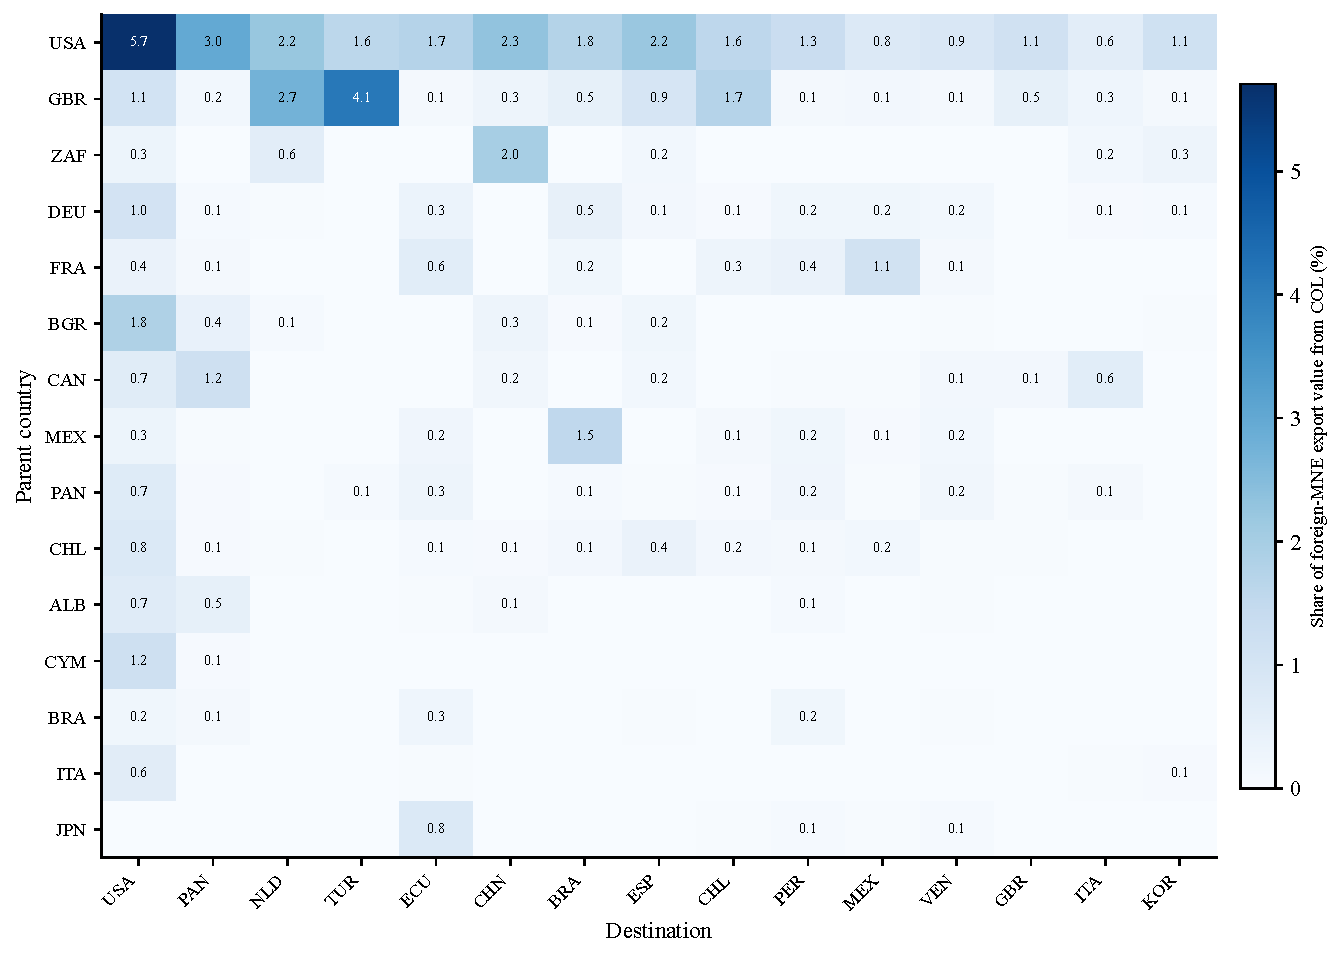
\includegraphics[width=1.0\textwidth,height=0.8\textheight,keepaspectratio]{figures/all/fig_wp1d_heatmap_country_cellpct_COL.pdf}%
  \caption{Colombia: Foreign-Multinational Exports by Parent Country and Destination}%
  \label{fig:c_hm_COL}%
  \par\vspace{2pt}%
  \parbox{0.92\textwidth}{\footnotesize %
  \textit{Notes:} Percent of the foreign-MNE export value of Colombia in each parent country and destination pair; fifteen largest parent countries and destinations.\\[3pt]%
  \textit{Source:} Authors' calculations based on customs data matched to Orbis and Dun \& Bradstreet.}%
  \end{figure}
% ---- Figure: Colombia: Share of Foreign-Multinational Exports Shipped to the Parent Country
\begin{figure}[H]\centering%
  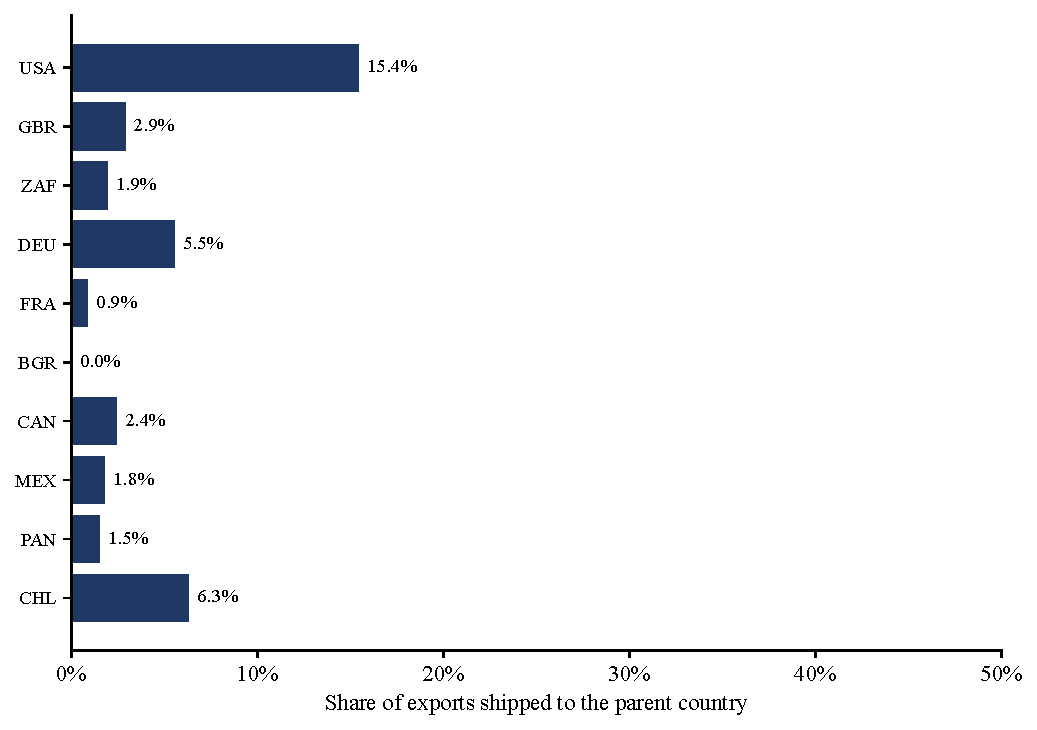
\includegraphics[width=0.85\textwidth,height=0.8\textheight,keepaspectratio]{figures/all/fig_wp1d_home_share_by_parent_COL.pdf}%
  \caption{Colombia: Share of Foreign-Multinational Exports Shipped to the Parent Country}%
  \label{fig:c_home_COL}%
  \par\vspace{2pt}%
  \parbox{0.92\textwidth}{\footnotesize %
  \textit{Notes:} Percent of each parent country's exports from Colombia shipped to that same country; ten largest parent countries.\\[3pt]%
  \textit{Source:} Authors' calculations based on customs data matched to Orbis and Dun \& Bradstreet.}%
  \end{figure}
% ---- Table: Colombia, Agriculture: Multinational Exports by Parent Region and Destination Region
\begin{table}[H]\centering\small%
  \caption{Colombia, Agriculture: Multinational Exports by Parent Region and Destination Region}%
  \label{tab:c_reg_COL_agro}%
  \adjustbox{max width=\textwidth, max totalheight=0.8\textheight}{\begin{tabular}{lrrrrrrrr}
\toprule
COL: parent region \ destination & Latin America & North America & Europe & Asia & Africa & Oceania & Rest of World & Total \\
\midrule
Latin America & 9.4 & 54.8 & 28.8 & 5.6 & 0.1 & 1.0 & 0.2 & 0.2 \\
North America & 51.4 & 30.1 & 11.2 & 6.6 & 0.5 & 0.2 & 0.1 & 0.2 \\
Europe & 12.6 & 46.2 & 29.4 & 10.8 & 0.3 & 0.7 & 0.0 & 0.7 \\
Asia & 7.4 & 45.3 & 24.0 & 19.3 & 3.3 & 0.7 & 0.0 & 0.2 \\
Africa & 3.5 & 55.6 & 34.3 & 4.8 & 0.0 & 1.8 & 0.0 & 0.0 \\
Oceania & 87.7 & 11.4 & 0.7 & 0.1 & 0.0 & 0.0 & 0.0 & 0.0 \\
Rest of World & 100.0 & 0.0 & 0.0 & 0.0 & 0.0 & 0.0 & 0.0 & 0.0 \\
Domestic MNEs & 19.6 & 37.1 & 27.6 & 14.1 & 1.1 & 0.5 & 0.0 & 1.0 \\
Local firms & 16.1 & 42.5 & 31.7 & 7.3 & 1.2 & 0.7 & 0.5 & 4.1 \\
\bottomrule
\end{tabular}
}%
  \par\vspace{3pt}%
  \begin{minipage}{0.95\textwidth}\footnotesize %
  \textit{Notes:} Percent of each group's agricultural exports from Colombia, by destination region (rows add to 100). Last column: the group's exports. Values are annual averages in US\$ billion.\\[3pt]%
  \textit{Source:} Authors' calculations based on customs data matched to Orbis and Dun \& Bradstreet.%
  \end{minipage}%
  \end{table}
% ---- Table: Colombia, Manufacturing: Multinational Exports by Parent Region and Destination Region
\begin{table}[H]\centering\small%
  \caption{Colombia, Manufacturing: Multinational Exports by Parent Region and Destination Region}%
  \label{tab:c_reg_COL_manufacturing}%
  \adjustbox{max width=\textwidth, max totalheight=0.8\textheight}{\begin{tabular}{lrrrrrrrr}
\toprule
COL: parent region \ destination & Latin America & North America & Europe & Asia & Africa & Oceania & Rest of World & Total \\
\midrule
Latin America & 69.7 & 22.2 & 2.2 & 4.1 & 0.3 & 0.0 & 1.5 & 1.2 \\
North America & 80.6 & 11.9 & 1.8 & 5.0 & 0.4 & 0.1 & 0.2 & 1.0 \\
Europe & 87.6 & 5.3 & 2.9 & 3.6 & 0.1 & 0.1 & 0.2 & 1.3 \\
Asia & 84.3 & 8.0 & 0.4 & 2.3 & 0.3 & 0.3 & 4.3 & 0.3 \\
Africa & 0.3 & 7.0 & 24.8 & 65.9 & 1.9 & 0.0 & 0.0 & 0.6 \\
Oceania & 99.6 & 0.1 & 0.0 & 0.0 & 0.2 & 0.0 & 0.0 & 0.0 \\
Rest of World & 73.2 & 26.8 & 0.0 & 0.0 & 0.0 & 0.0 & 0.0 & 0.0 \\
Domestic MNEs & 79.7 & 13.5 & 4.7 & 1.2 & 0.3 & 0.2 & 0.3 & 0.8 \\
Local firms & 66.1 & 16.2 & 5.8 & 9.5 & 0.5 & 0.1 & 1.8 & 3.0 \\
\bottomrule
\end{tabular}
}%
  \par\vspace{3pt}%
  \begin{minipage}{0.95\textwidth}\footnotesize %
  \textit{Notes:} Percent of each group's manufacturing exports from Colombia, by destination region (rows add to 100). Last column: the group's exports. Values are annual averages in US\$ billion.\\[3pt]%
  \textit{Source:} Authors' calculations based on customs data matched to Orbis and Dun \& Bradstreet.%
  \end{minipage}%
  \end{table}
% ---- Table: Colombia, Mining and Fuels: Multinational Exports by Parent Region and Destination Region
\begin{table}[H]\centering\small%
  \caption{Colombia, Mining and Fuels: Multinational Exports by Parent Region and Destination Region}%
  \label{tab:c_reg_COL_mining}%
  \adjustbox{max width=\textwidth, max totalheight=0.8\textheight}{\begin{tabular}{lrrrrrrrr}
\toprule
COL: parent region \ destination & Latin America & North America & Europe & Asia & Africa & Oceania & Rest of World & Total \\
\midrule
Latin America & 28.4 & 30.3 & 18.3 & 19.1 & 0.0 & 3.4 & 0.6 & 0.6 \\
North America & 31.9 & 17.0 & 32.5 & 18.0 & 0.5 & 0.0 & 0.0 & 4.4 \\
Europe & 23.2 & 17.5 & 50.5 & 7.3 & 0.6 & 0.0 & 0.8 & 3.0 \\
Asia & 4.3 & 6.0 & 83.6 & 3.1 & 0.2 & 0.0 & 2.8 & 0.0 \\
Africa & 0.7 & 81.6 & 0.2 & 1.8 & 0.0 & 0.0 & 15.8 & 0.0 \\
Oceania & 7.3 & 16.9 & 51.2 & 21.7 & 0.0 & 0.0 & 2.9 & 0.0 \\
Domestic MNEs & 23.3 & 46.4 & 6.8 & 22.3 & 0.8 & 0.0 & 0.4 & 15.4 \\
Local firms & 23.5 & 35.2 & 28.3 & 9.0 & 0.5 & 0.0 & 3.5 & 4.1 \\
\bottomrule
\end{tabular}
}%
  \par\vspace{3pt}%
  \begin{minipage}{0.95\textwidth}\footnotesize %
  \textit{Notes:} Percent of each group's mining and fuels exports from Colombia, by destination region (rows add to 100). Last column: the group's exports. Values are annual averages in US\$ billion.\\[3pt]%
  \textit{Source:} Authors' calculations based on customs data matched to Orbis and Dun \& Bradstreet.%
  \end{minipage}%
  \end{table}
% ---- Table: Colombia, Other Goods: Multinational Exports by Parent Region and Destination Region
\begin{table}[H]\centering\small%
  \caption{Colombia, Other Goods: Multinational Exports by Parent Region and Destination Region}%
  \label{tab:c_reg_COL_rest}%
  \adjustbox{max width=\textwidth, max totalheight=0.8\textheight}{\begin{tabular}{lrrrrrrrr}
\toprule
COL: parent region \ destination & Latin America & North America & Europe & Asia & Africa & Oceania & Rest of World & Total \\
\midrule
Latin America & 55.5 & 15.0 & 20.5 & 9.0 & 0.0 & 0.0 & 0.0 & 0.0 \\
North America & 7.7 & 83.7 & 4.8 & 2.7 & 1.1 & 0.0 & 0.0 & 0.0 \\
Europe & 42.9 & 34.2 & 20.8 & 1.3 & 0.8 & 0.0 & 0.1 & 0.0 \\
Asia & 96.5 & 0.8 & 0.2 & 2.4 & 0.0 & 0.0 & 0.0 & 0.0 \\
Africa & 39.4 & 27.2 & 23.7 & 6.8 & 0.0 & 2.8 & 0.0 & 0.0 \\
Rest of World & 0.0 & 100.0 & 0.0 & 0.0 & 0.0 & 0.0 & 0.0 & 0.0 \\
Domestic MNEs & 77.4 & 12.9 & 8.6 & 0.0 & 1.0 & 0.2 & 0.0 & 0.0 \\
Local firms & 48.1 & 28.0 & 16.8 & 4.9 & 1.4 & 0.7 & 0.0 & 0.0 \\
\bottomrule
\end{tabular}
}%
  \par\vspace{3pt}%
  \begin{minipage}{0.95\textwidth}\footnotesize %
  \textit{Notes:} Percent of each group's exports from Colombia, by destination region (rows add to 100). Last column: the group's exports. Values are annual averages in US\$ billion.\\[3pt]%
  \textit{Source:} Authors' calculations based on customs data matched to Orbis and Dun \& Bradstreet.%
  \end{minipage}%
  \end{table}

\subsection{Products}
% ---- Table: Colombia: Fifteen Largest Export Products
\begin{table}[H]\centering\footnotesize%
  \caption{Colombia: Fifteen Largest Export Products}%
  \label{tab:c_hs6_COL}%
  \adjustbox{max width=\textwidth, max totalheight=0.8\textheight}{\begin{tabular}{@{}l p{6.4cm} r r r r l@{}}
\toprule
HS6 & Description & US\$bn/yr & Foreign (\%) & Domestic (\%) & Local (\%) & Leading parent \\
\midrule
270900 & Petroleum oils and oils obt. from bituminous mins., crude & 16.1 & 17 & 81 & 2 & USA (0.62) \\
270112 & Bituminous coal, whether/\allowbreak{}not pulverised but not agglomerated & 5.7 & 77 & 0 & 22 & GBR (0.49) \\
090111 & Coffee, not roasted, not decaffeinated & 2.4 & 39 & 21 & 40 & DEU (0.42) \\
271019 & Petroleum oils and oils obtained from bituminous minerals (other than crude) and preparations ... & 2.0 & 2 & 83 & 15 & ALB (0.35) \\
710812 & Gold (incl. gold plated with platinum), in unwrought forms (excl. powder) & 2.0 & 23 & 11 & 66 & PAN (0.37) \\
080390 & Bananas, fresh or dried (excl. plantains) [HS2012 code] & 0.7 & 14 & 0 & 86 & GRC (0.68) \\
060319 & Cut flowers and flower buds of a kind suit. for bouquets/\allowbreak{}ornamental purposes(excl. of 0603.11-... & 0.6 & 21 & 18 & 61 & ARG (0.30) \\
271012 & Light petroleum oils and preparations [HS2012 code] & 0.6 & 50 & 35 & 14 & CHL (0.84) \\
720260 & Ferro-nickel, in granular/\allowbreak{}powder form & 0.6 & 100 & 0 & 0 & ZAF (1.00) \\
270400 & Coke and semi-coke of coal/\allowbreak{}lignite/\allowbreak{}peat, whether/\allowbreak{}not agglomerated; retort carbon & 0.6 & 40 & 0 & 59 & PAN (0.54) \\
060311 & Fresh roses & 0.3 & 21 & 8 & 71 & BGR (0.32) \\
390410 & Poly(vinyl chloride), not mixed with any other substance, in primary forms & 0.3 & 100 & 0 & 0 & MEX (1.00) \\
170199 & Cane/\allowbreak{}beet sugar and chemically pure sucrose, in solid form, not containing added flavouring/\allowbreak{}co... & 0.3 & 22 & 0 & 78 & USA (1.00) \\
390210 & Polypropylene, in primary forms & 0.3 & 0 & 0 & 100 & USA (0.74) \\
870323 & Vehicles (excl. of 87.02 and 8703.10) principally designed for the transportof persons, with s... & 0.3 & 99 & 0 & 0 & FRA (0.99) \\
\bottomrule
\end{tabular}
}%
  \par\vspace{3pt}%
  \begin{minipage}{0.95\textwidth}\footnotesize %
  \textit{Notes:} Fifteen largest HS6 products exported by Colombia. Foreign, domestic and local: percent of the product's export value. Leading parent: largest parent country and its share of the product's foreign-MNE exports. Values are annual averages in US\$ billion.\\[3pt]%
  \textit{Source:} Authors' calculations based on customs data matched to Orbis and Dun \& Bradstreet.%
  \end{minipage}%
  \end{table}
% ---- Table: Colombia, Agriculture: Fifteen Largest Export Products
\begin{table}[H]\centering\footnotesize%
  \caption{Colombia, Agriculture: Fifteen Largest Export Products}%
  \label{tab:c_hs6_COL_agro}%
  \adjustbox{max width=\textwidth, max totalheight=0.8\textheight}{\begin{tabular}{@{}l p{6.4cm} r r r r l@{}}
\toprule
HS6 & Description & US\$bn/yr & Foreign (\%) & Domestic (\%) & Local (\%) & Leading parent \\
\midrule
090111 & Coffee, not roasted, not decaffeinated & 2.4 & 39 & 21 & 40 & DEU (0.42) \\
080390 & Bananas, fresh or dried (excl. plantains) [HS2012 code] & 0.7 & 14 & 0 & 86 & GRC (0.68) \\
060319 & Cut flowers and flower buds of a kind suit. for bouquets/\allowbreak{}ornamental purposes(excl. of 0603.11-... & 0.6 & 21 & 18 & 61 & ARG (0.30) \\
060311 & Fresh roses & 0.3 & 21 & 8 & 71 & BGR (0.32) \\
170199 & Cane/\allowbreak{}beet sugar and chemically pure sucrose, in solid form, not containing added flavouring/\allowbreak{}co... & 0.3 & 22 & 0 & 78 & USA (1.00) \\
210111 & Extracts, essences and concentrates of coffee & 0.2 & 22 & 49 & 29 & CHE (0.72) \\
151110 & Palm oil, crude & 0.2 & 44 & 0 & 56 & USA (0.76) \\
060312 & Fresh carnations & 0.2 & 23 & 3 & 75 & BGR (0.31) \\
170490 & Sugar confectionery other than chewing gum (incl. white chocolate), not containing cocoa & 0.2 & 10 & 53 & 38 & USA (0.77) \\
060314 & Fresh chrysanthemums & 0.1 & 14 & 6 & 80 & ESP (0.26) \\
080300 & Bananas, incl. plantains, fresh/\allowbreak{}dried & 0.1 & 14 & 0 & 86 & GRC (0.61) \\
010229 & Live bovine animals other than pure-bred breeding animals [HS 2007 line 010... & 0.1 & 9 & 6 & 85 & BGR (0.43) \\
170114 & Cane sugar, raw, in solid form, not containing added flavouring/\allowbreak{}colouring matter [later HS rev... & 0.1 & 2 & 1 & 98 & USA (0.92) \\
210690 & Food preparations, n.e.s. & 0.1 & 50 & 4 & 46 & URY (0.27) \\
081090 & Fresh fruit, n.e.s. in Ch. 8 & 0.1 & 23 & 0 & 77 & BGR (0.54) \\
\bottomrule
\end{tabular}
}%
  \par\vspace{3pt}%
  \begin{minipage}{0.95\textwidth}\footnotesize %
  \textit{Notes:} Fifteen largest agricultural HS6 products exported by Colombia. Foreign, domestic and local: percent of the product's export value. Leading parent: largest parent country and its share of the product's foreign-MNE exports. Values are annual averages in US\$ billion.\\[3pt]%
  \textit{Source:} Authors' calculations based on customs data matched to Orbis and Dun \& Bradstreet.%
  \end{minipage}%
  \end{table}
% ---- Table: Colombia, Manufacturing: Fifteen Largest Export Products
\begin{table}[H]\centering\footnotesize%
  \caption{Colombia, Manufacturing: Fifteen Largest Export Products}%
  \label{tab:c_hs6_COL_manufacturing}%
  \adjustbox{max width=\textwidth, max totalheight=0.8\textheight}{\begin{tabular}{@{}l p{6.4cm} r r r r l@{}}
\toprule
HS6 & Description & US\$bn/yr & Foreign (\%) & Domestic (\%) & Local (\%) & Leading parent \\
\midrule
720260 & Ferro-nickel, in granular/\allowbreak{}powder form & 0.60 & 100 & 0 & 0 & ZAF (1.00) \\
390410 & Poly(vinyl chloride), not mixed with any other substance, in primary forms & 0.30 & 100 & 0 & 0 & MEX (1.00) \\
390210 & Polypropylene, in primary forms & 0.27 & 0 & 0 & 100 & USA (0.74) \\
870323 & Vehicles (excl. of 87.02 and 8703.10) principally designed for the transportof persons, with s... & 0.26 & 99 & 0 & 0 & FRA (0.99) \\
740400 & Copper waste and scrap & 0.25 & 32 & 0 & 67 & BGR (0.56) \\
300490 & Medicaments (excluding goods of heading 30.02/\allowbreak{}30.05/\allowbreak{}30.06/\allowbreak{}3004.10-3004.50) consisting of mixed... & 0.24 & 60 & 14 & 26 & USA (0.24) \\
380892 & Fungicides, put up in forms/\allowbreak{}packings for retail sale/\allowbreak{}as preparations/\allowbreak{}articles  & 0.18 & 99 & 0 & 1 & USA (0.50) \\
390230 & Propylene copolymers, in primary forms & 0.15 & 0 & 0 & 100 & USA (0.54) \\
761010 & Doors, windows and their frames and thresholds for doors, of aluminium & 0.12 & 99 & 0 & 1 & CYM (1.00) \\
380891 & Insecticides, put up in forms/\allowbreak{}packings for retail sale/\allowbreak{}as preparations/\allowbreak{}articles  & 0.12 & 98 & 0 & 2 & DEU (0.81) \\
961900 & Sanitary towels and tampons, napkins and napkin liners for babies and similar sanitary article... & 0.10 & 97 & 1 & 2 & USA (0.60) \\
850710 & Electric accumulators, incl. separators therefor, whether/\allowbreak{}not rectangular (incl. square), lead... & 0.10 & 8 & 0 & 92 & ALB (0.98) \\
330300 & Perfumes and toilet waters & 0.09 & 31 & 52 & 17 & PAN (0.56) \\
330499 & Beauty/\allowbreak{}make-up preparations and preparations for the care of the skin (excl. meds.; excl. of 3... & 0.09 & 42 & 37 & 20 & USA (0.41) \\
841810 & Combined refrigerator-freezers, fitted with separate external doors, electric/\allowbreak{}other & 0.07 & 80 & 0 & 20 & MEX (0.99) \\
\bottomrule
\end{tabular}
}%
  \par\vspace{3pt}%
  \begin{minipage}{0.95\textwidth}\footnotesize %
  \textit{Notes:} Fifteen largest manufacturing HS6 products exported by Colombia. Foreign, domestic and local: percent of the product's export value. Leading parent: largest parent country and its share of the product's foreign-MNE exports. Values are annual averages in US\$ billion.\\[3pt]%
  \textit{Source:} Authors' calculations based on customs data matched to Orbis and Dun \& Bradstreet.%
  \end{minipage}%
  \end{table}
% ---- Table: Colombia, Mining and Fuels: Fifteen Largest Export Products
\begin{table}[H]\centering\footnotesize%
  \caption{Colombia, Mining and Fuels: Fifteen Largest Export Products}%
  \label{tab:c_hs6_COL_mining}%
  \adjustbox{max width=\textwidth, max totalheight=0.8\textheight}{\begin{tabular}{@{}l p{6.4cm} r r r r l@{}}
\toprule
HS6 & Description & US\$bn/yr & Foreign (\%) & Domestic (\%) & Local (\%) & Leading parent \\
\midrule
270900 & Petroleum oils and oils obt. from bituminous mins., crude & 16.1 & 17 & 81 & 2 & USA (0.62) \\
270112 & Bituminous coal, whether/\allowbreak{}not pulverised but not agglomerated & 5.7 & 77 & 0 & 22 & GBR (0.49) \\
271019 & Petroleum oils and oils obtained from bituminous minerals (other than crude) and preparations ... & 2.0 & 2 & 83 & 15 & ALB (0.35) \\
710812 & Gold (incl. gold plated with platinum), in unwrought forms (excl. powder) & 2.0 & 23 & 11 & 66 & PAN (0.37) \\
271012 & Light petroleum oils and preparations [HS2012 code] & 0.6 & 50 & 35 & 14 & CHL (0.84) \\
270400 & Coke and semi-coke of coal/\allowbreak{}lignite/\allowbreak{}peat, whether/\allowbreak{}not agglomerated; retort carbon & 0.6 & 40 & 0 & 59 & PAN (0.54) \\
271011 & Light petroleum oils and preparations & 0.2 & 38 & 61 & 1 & CHL (0.46) \\
710813 & Gold (incl. gold plated with platinum), non-monetary, in semi-manufactured forms & 0.1 & 1 & 0 & 99 & ESP (0.92) \\
271121 & Natural gas, in gaseous state & 0.1 & 37 & 63 & 0 & USA (1.00) \\
710391 & Rubies, sapphires and emeralds, worked othw. than simply sawn/\allowbreak{}roughly shaped but not strung/\allowbreak{}mo... & 0.1 & 22 & 1 & 77 & BGR (0.67) \\
271600 & Electrical energy (optional heading) & 0.1 & 33 & 0 & 67 & CAN (1.00) \\
711011 & Platinum, unwrought/\allowbreak{}in powder form & 0.0 & 10 & 42 & 48 & FRA (0.85) \\
260300 & Copper ores and concentrates & 0.0 & 99 & 0 & 1 & CAN (1.00) \\
711719 & Imitation jewellery, of base metal, whether/\allowbreak{}not plated with precious metal, other than cuff-li... & 0.0 & 80 & 2 & 17 & ALB (0.64) \\
271311 & Petroleum coke, not calcined & 0.0 & 0 & 39 & 61 & ESP (1.00) \\
\bottomrule
\end{tabular}
}%
  \par\vspace{3pt}%
  \begin{minipage}{0.95\textwidth}\footnotesize %
  \textit{Notes:} Fifteen largest mining and fuels HS6 products exported by Colombia. Foreign, domestic and local: percent of the product's export value. Leading parent: largest parent country and its share of the product's foreign-MNE exports. Values are annual averages in US\$ billion.\\[3pt]%
  \textit{Source:} Authors' calculations based on customs data matched to Orbis and Dun \& Bradstreet.%
  \end{minipage}%
  \end{table}
% ---- Table: Colombia, Other Goods: Fifteen Largest Export Products
\begin{table}[H]\centering\footnotesize%
  \caption{Colombia, Other Goods: Fifteen Largest Export Products}%
  \label{tab:c_hs6_COL_rest}%
  \adjustbox{max width=\textwidth, max totalheight=0.8\textheight}{\begin{tabular}{@{}l p{6.4cm} r r r r l@{}}
\toprule
HS6 & Description & US\$bn/yr & Foreign (\%) & Domestic (\%) & Local (\%) & Leading parent \\
\midrule
980500 & National /\allowbreak{} special customs line (no HS description) & 0.01 & 9 & 0 & 91 & USA (0.82) \\
980110 & National /\allowbreak{} special customs line (no HS description) & 0.00 & 91 & 0 & 9 & JPN (1.00) \\
980190 & National /\allowbreak{} special customs line (no HS description) & 0.00 & 60 & 7 & 33 & JPN (1.00) \\
980300 & National /\allowbreak{} special customs line (no HS description) & 0.00 & 82 & 1 & 17 & ALB (0.71) \\
980720 & National /\allowbreak{} special customs line (no HS description) & 0.00 & 34 & 32 & 34 & USA (0.68) \\
980400 & National /\allowbreak{} special customs line (no HS description) & 0.00 & 0 & 0 & 100 & -- \\
980600 & National /\allowbreak{} special customs line (no HS description) & 0.00 & 5 & 1 & 94 & HUN (0.67) \\
980710 & National /\allowbreak{} special customs line (no HS description) & 0.00 & 0 & 0 & 100 & -- \\
\bottomrule
\end{tabular}
}%
  \par\vspace{3pt}%
  \begin{minipage}{0.95\textwidth}\footnotesize %
  \textit{Notes:} Fifteen largest HS6 products exported by Colombia. Foreign, domestic and local: percent of the product's export value. Leading parent: largest parent country and its share of the product's foreign-MNE exports. Values are annual averages in US\$ billion.\\[3pt]%
  \textit{Source:} Authors' calculations based on customs data matched to Orbis and Dun \& Bradstreet.%
  \end{minipage}%
  \end{table}

\section{Costa Rica}\label{sec:c_CRI}

\subsection{Parents and Destinations}
% ---- Table: Costa Rica: Multinational Exports by Parent Region and Destination Region
\begin{table}[H]\centering\small%
  \caption{Costa Rica: Multinational Exports by Parent Region and Destination Region}%
  \label{tab:c_reg_CRI}%
  \adjustbox{max width=\textwidth, max totalheight=0.8\textheight}{\begin{tabular}{lrrrrrrrr}
\toprule
CRI: parent region \ destination & Latin America & North America & Europe & Asia & Africa & Oceania & Rest of World & Total \\
\midrule
Latin America & 62.4 & 26.6 & 9.3 & 1.5 & 0.1 & 0.0 & 0.0 & 0.6 \\
North America & 24.7 & 47.2 & 12.2 & 15.8 & 0.0 & 0.1 & 0.0 & 3.2 \\
Europe & 44.2 & 28.6 & 24.3 & 2.3 & 0.1 & 0.4 & 0.0 & 1.2 \\
Asia & 19.7 & 50.9 & 22.9 & 6.0 & 0.5 & 0.0 & 0.0 & 0.8 \\
Africa & 55.4 & 21.0 & 23.1 & 0.4 & 0.0 & 0.0 & 0.0 & 0.0 \\
Rest of World & 91.1 & 0.0 & 0.0 & 8.9 & 0.0 & 0.0 & 0.0 & 0.0 \\
Domestic MNEs & 20.7 & 51.1 & 19.7 & 6.3 & 0.3 & 1.9 & 0.0 & 0.4 \\
Local firms & 32.1 & 35.4 & 26.3 & 5.4 & 0.3 & 0.5 & 0.0 & 3.8 \\
\bottomrule
\end{tabular}
}%
  \par\vspace{3pt}%
  \begin{minipage}{0.95\textwidth}\footnotesize %
  \textit{Notes:} Percent of each group's exports from Costa Rica, by destination region (rows add to 100). Last column: the group's exports. Values are annual averages in US\$ billion.\\[3pt]%
  \textit{Source:} Authors' calculations based on customs data matched to Orbis and Dun \& Bradstreet.%
  \end{minipage}%
  \end{table}
% ---- Figure: Costa Rica: Foreign-Multinational Exports by Parent Country and Destination
\begin{figure}[H]\centering%
  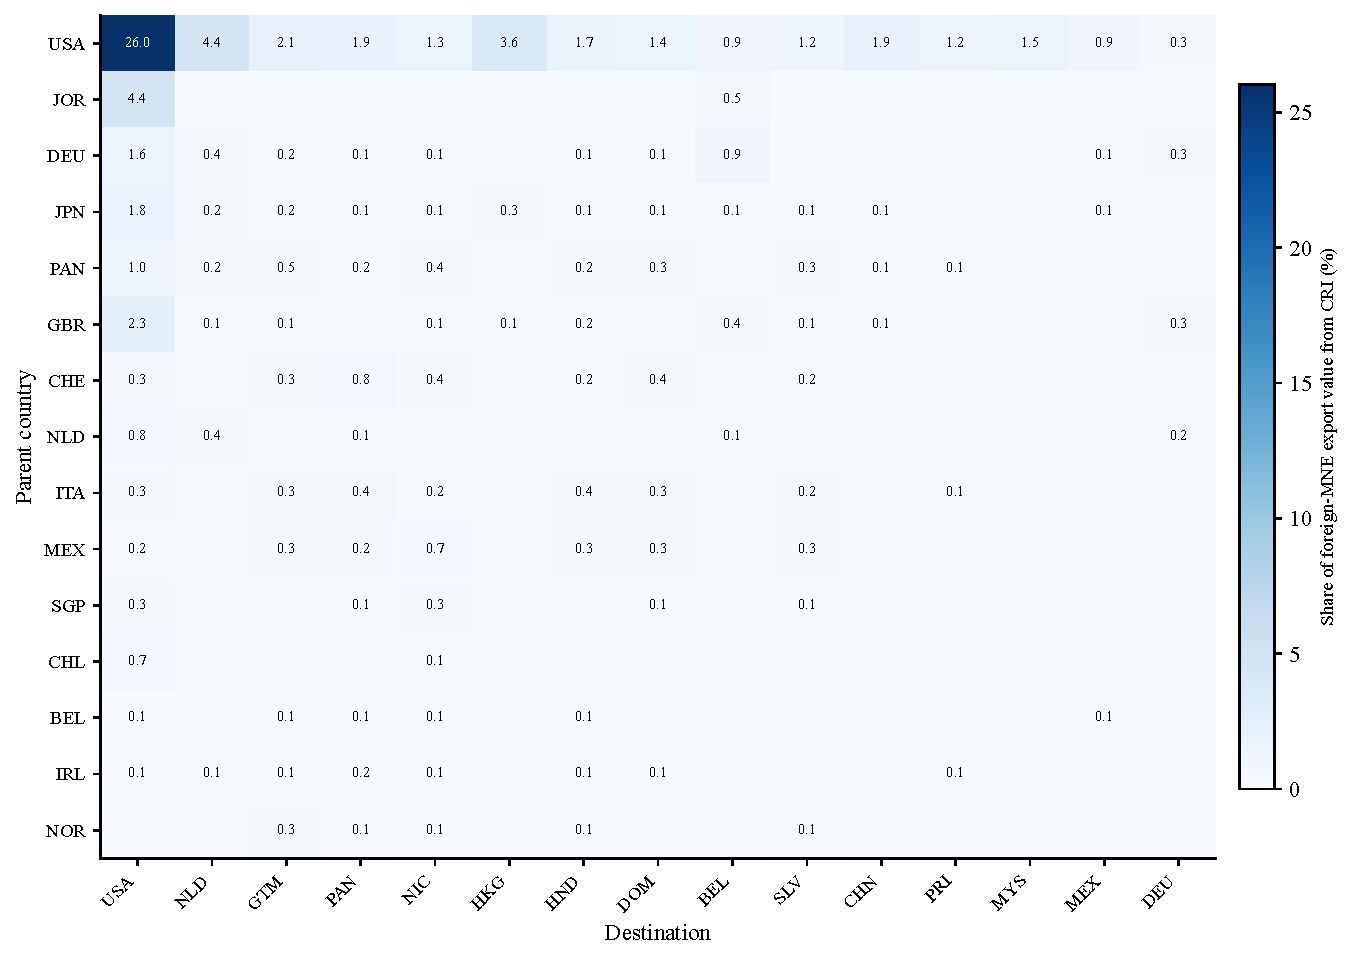
\includegraphics[width=1.0\textwidth,height=0.8\textheight,keepaspectratio]{figures/all/fig_wp1d_heatmap_country_cellpct_CRI.pdf}%
  \caption{Costa Rica: Foreign-Multinational Exports by Parent Country and Destination}%
  \label{fig:c_hm_CRI}%
  \par\vspace{2pt}%
  \parbox{0.92\textwidth}{\footnotesize %
  \textit{Notes:} Percent of the foreign-MNE export value of Costa Rica in each parent country and destination pair; fifteen largest parent countries and destinations.\\[3pt]%
  \textit{Source:} Authors' calculations based on customs data matched to Orbis and Dun \& Bradstreet.}%
  \end{figure}
% ---- Figure: Costa Rica: Share of Foreign-Multinational Exports Shipped to the Parent Country
\begin{figure}[H]\centering%
  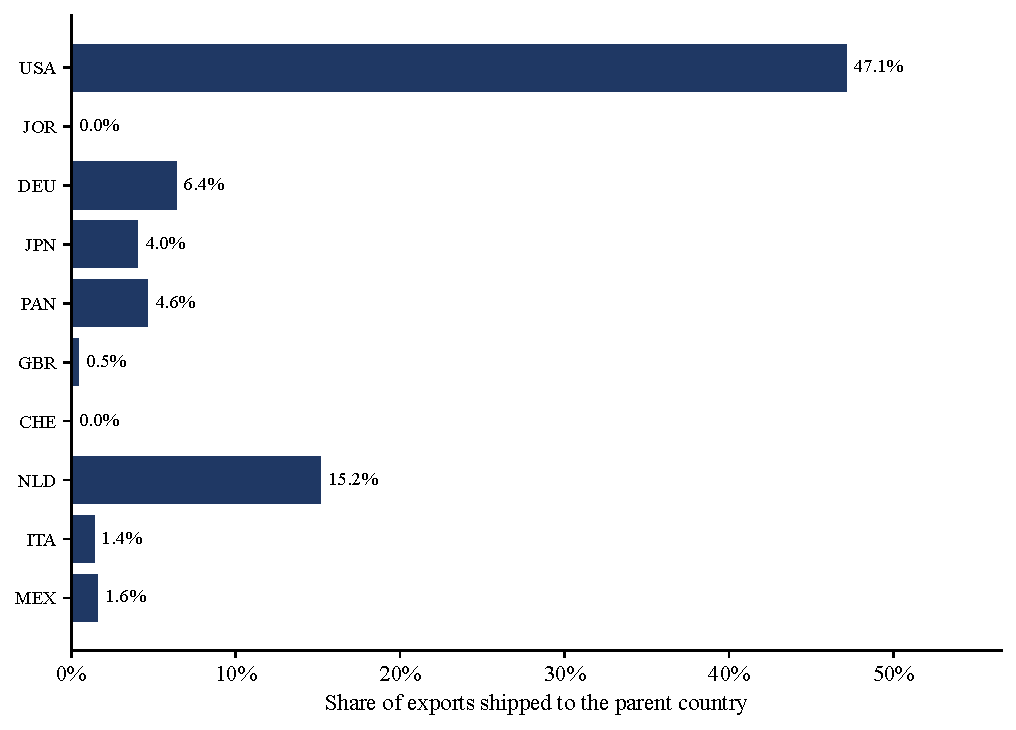
\includegraphics[width=0.85\textwidth,height=0.8\textheight,keepaspectratio]{figures/all/fig_wp1d_home_share_by_parent_CRI.pdf}%
  \caption{Costa Rica: Share of Foreign-Multinational Exports Shipped to the Parent Country}%
  \label{fig:c_home_CRI}%
  \par\vspace{2pt}%
  \parbox{0.92\textwidth}{\footnotesize %
  \textit{Notes:} Percent of each parent country's exports from Costa Rica shipped to that same country; ten largest parent countries.\\[3pt]%
  \textit{Source:} Authors' calculations based on customs data matched to Orbis and Dun \& Bradstreet.}%
  \end{figure}
% ---- Table: Costa Rica, Agriculture: Multinational Exports by Parent Region and Destination Region
\begin{table}[H]\centering\small%
  \caption{Costa Rica, Agriculture: Multinational Exports by Parent Region and Destination Region}%
  \label{tab:c_reg_CRI_agro}%
  \adjustbox{max width=\textwidth, max totalheight=0.8\textheight}{\begin{tabular}{lrrrrrrrr}
\toprule
CRI: parent region \ destination & Latin America & North America & Europe & Asia & Africa & Oceania & Rest of World & Total \\
\midrule
Latin America & 27.8 & 49.0 & 19.6 & 3.5 & 0.1 & 0.0 & 0.0 & 0.2 \\
North America & 64.5 & 23.1 & 12.1 & 0.1 & 0.2 & 0.0 & 0.0 & 0.6 \\
Europe & 22.2 & 28.8 & 44.8 & 3.0 & 0.2 & 0.9 & 0.0 & 0.5 \\
Asia & 0.4 & 61.2 & 36.5 & 1.3 & 0.6 & 0.0 & 0.0 & 0.4 \\
Africa & 18.1 & 30.4 & 50.6 & 1.0 & 0.0 & 0.0 & 0.0 & 0.0 \\
Rest of World & 0.0 & 0.0 & 0.0 & 100.0 & 0.0 & 0.0 & 0.0 & 0.0 \\
Domestic MNEs & 22.8 & 41.0 & 34.6 & 0.3 & 0.9 & 0.4 & 0.0 & 0.1 \\
Local firms & 27.3 & 33.2 & 35.3 & 3.3 & 0.3 & 0.6 & 0.0 & 2.3 \\
\bottomrule
\end{tabular}
}%
  \par\vspace{3pt}%
  \begin{minipage}{0.95\textwidth}\footnotesize %
  \textit{Notes:} Percent of each group's agricultural exports from Costa Rica, by destination region (rows add to 100). Last column: the group's exports. Values are annual averages in US\$ billion.\\[3pt]%
  \textit{Source:} Authors' calculations based on customs data matched to Orbis and Dun \& Bradstreet.%
  \end{minipage}%
  \end{table}
% ---- Table: Costa Rica, Manufacturing: Multinational Exports by Parent Region and Destination Region
\begin{table}[H]\centering\small%
  \caption{Costa Rica, Manufacturing: Multinational Exports by Parent Region and Destination Region}%
  \label{tab:c_reg_CRI_manufacturing}%
  \adjustbox{max width=\textwidth, max totalheight=0.8\textheight}{\begin{tabular}{lrrrrrrrr}
\toprule
CRI: parent region \ destination & Latin America & North America & Europe & Asia & Africa & Oceania & Rest of World & Total \\
\midrule
Latin America & 78.6 & 16.3 & 4.4 & 0.5 & 0.1 & 0.1 & 0.0 & 0.4 \\
North America & 14.6 & 53.3 & 12.3 & 19.8 & 0.0 & 0.1 & 0.0 & 2.5 \\
Europe & 59.4 & 28.2 & 10.4 & 1.9 & 0.0 & 0.1 & 0.0 & 0.7 \\
Asia & 45.4 & 37.2 & 4.7 & 12.1 & 0.5 & 0.1 & 0.0 & 0.3 \\
Africa & 86.8 & 13.2 & 0.0 & 0.0 & 0.0 & 0.0 & 0.0 & 0.0 \\
Rest of World & 100.0 & 0.0 & 0.0 & 0.0 & 0.0 & 0.0 & 0.0 & 0.0 \\
Domestic MNEs & 20.2 & 53.3 & 16.5 & 7.6 & 0.2 & 2.2 & 0.0 & 0.3 \\
Local firms & 40.4 & 37.5 & 12.6 & 8.9 & 0.2 & 0.4 & 0.0 & 1.4 \\
\bottomrule
\end{tabular}
}%
  \par\vspace{3pt}%
  \begin{minipage}{0.95\textwidth}\footnotesize %
  \textit{Notes:} Percent of each group's manufacturing exports from Costa Rica, by destination region (rows add to 100). Last column: the group's exports. Values are annual averages in US\$ billion.\\[3pt]%
  \textit{Source:} Authors' calculations based on customs data matched to Orbis and Dun \& Bradstreet.%
  \end{minipage}%
  \end{table}
% ---- Table: Costa Rica, Mining and Fuels: Multinational Exports by Parent Region and Destination Region
\begin{table}[H]\centering\small%
  \caption{Costa Rica, Mining and Fuels: Multinational Exports by Parent Region and Destination Region}%
  \label{tab:c_reg_CRI_mining}%
  \adjustbox{max width=\textwidth, max totalheight=0.8\textheight}{\begin{tabular}{lrrrrrrrr}
\toprule
CRI: parent region \ destination & Latin America & North America & Europe & Asia & Africa & Oceania & Rest of World & Total \\
\midrule
Latin America & 99.9 & 0.0 & 0.0 & 0.0 & 0.0 & 0.0 & 0.0 & 0.0 \\
North America & 8.0 & 90.1 & 0.4 & 1.5 & 0.0 & 0.0 & 0.0 & 0.0 \\
Europe & 63.9 & 36.0 & 0.0 & 0.0 & 0.0 & 0.0 & 0.0 & 0.0 \\
Asia & 78.1 & 21.3 & 0.6 & 0.0 & 0.0 & 0.0 & 0.0 & 0.0 \\
Domestic MNEs & 75.4 & 6.0 & 18.5 & 0.0 & 0.0 & 0.0 & 0.0 & 0.0 \\
Local firms & 19.3 & 74.7 & 4.6 & 1.4 & 0.0 & 0.0 & 0.0 & 0.1 \\
\bottomrule
\end{tabular}
}%
  \par\vspace{3pt}%
  \begin{minipage}{0.95\textwidth}\footnotesize %
  \textit{Notes:} Percent of each group's mining and fuels exports from Costa Rica, by destination region (rows add to 100). Last column: the group's exports. Values are annual averages in US\$ billion.\\[3pt]%
  \textit{Source:} Authors' calculations based on customs data matched to Orbis and Dun \& Bradstreet.%
  \end{minipage}%
  \end{table}
% ---- Table: Costa Rica, Other Goods: Multinational Exports by Parent Region and Destination Region
\begin{table}[H]\centering\small%
  \caption{Costa Rica, Other Goods: Multinational Exports by Parent Region and Destination Region}%
  \label{tab:c_reg_CRI_rest}%
  \adjustbox{max width=\textwidth, max totalheight=0.8\textheight}{\begin{tabular}{lrr}
\toprule
CRI: parent region \ destination & North America & Total \\
\midrule
\bottomrule
\end{tabular}
}%
  \par\vspace{3pt}%
  \begin{minipage}{0.95\textwidth}\footnotesize %
  \textit{Notes:} Percent of each group's exports from Costa Rica, by destination region (rows add to 100). Last column: the group's exports. Values are annual averages in US\$ billion.\\[3pt]%
  \textit{Source:} Authors' calculations based on customs data matched to Orbis and Dun \& Bradstreet.%
  \end{minipage}%
  \end{table}

\subsection{Products}
% ---- Table: Costa Rica: Fifteen Largest Export Products
\begin{table}[H]\centering\footnotesize%
  \caption{Costa Rica: Fifteen Largest Export Products}%
  \label{tab:c_hs6_CRI}%
  \adjustbox{max width=\textwidth, max totalheight=0.8\textheight}{\begin{tabular}{@{}l p{6.4cm} r r r r l@{}}
\toprule
HS6 & Description & US\$bn/yr & Foreign (\%) & Domestic (\%) & Local (\%) & Leading parent \\
\midrule
901839 & Catheters, cannulae and the like & 0.86 & 89 & 0 & 11 & USA (0.97) \\
080430 & Pineapples, fresh/\allowbreak{}dried & 0.85 & 43 & 0 & 57 & JOR (0.48) \\
854231 & Electronic integrated  circuits, processors and controllers, whether/\allowbreak{}not combined with memorie... & 0.76 & 100 & 0 & 0 & USA (0.98) \\
080390 & Bananas, fresh or dried (excl. plantains) [HS2012 code] & 0.75 & 51 & 2 & 47 & JOR (0.45) \\
901890 & Instruments and appliances used in medical/\allowbreak{}surgical/\allowbreak{}veterinary sciences, incl. other electro-m... & 0.60 & 79 & 1 & 21 & USA (0.62) \\
210690 & Food preparations, n.e.s. & 0.37 & 95 & 0 & 5 & USA (0.96) \\
902139 & Artificial parts of the body other than teeth, dental fittings and joints & 0.37 & 10 & 61 & 29 & VGB (0.47) \\
090111 & Coffee, not roasted, not decaffeinated & 0.31 & 46 & 0 & 54 & DEU (0.85) \\
080300 & Bananas, incl. plantains, fresh/\allowbreak{}dried & 0.16 & 49 & 4 & 46 & JOR (0.52) \\
300490 & Medicaments (excluding goods of heading 30.02/\allowbreak{}30.05/\allowbreak{}30.06/\allowbreak{}3004.10-3004.50) consisting of mixed... & 0.15 & 65 & 3 & 32 & CHE (0.49) \\
401110 & New pneumatic tyres, of rubber, of a kind used on motor cars (incl. station wagons and racing ... & 0.13 & 64 & 0 & 36 & JPN (1.00) \\
854449 & Other electric conductors, for a voltage not > 1,000 V, not fitted with connectors & 0.12 & 100 & 0 & 0 & ITA (0.99) \\
151110 & Palm oil, crude & 0.11 & 0 & 0 & 100 & -- \\
961900 & Sanitary towels and tampons, napkins and napkin liners for babies and similar sanitary article... & 0.10 & 100 & 0 & 0 & USA (1.00) \\
847330 & Parts and accessories of the machines of heading 84.71 & 0.09 & 98 & 0 & 2 & USA (1.00) \\
\bottomrule
\end{tabular}
}%
  \par\vspace{3pt}%
  \begin{minipage}{0.95\textwidth}\footnotesize %
  \textit{Notes:} Fifteen largest HS6 products exported by Costa Rica. Foreign, domestic and local: percent of the product's export value. Leading parent: largest parent country and its share of the product's foreign-MNE exports. Values are annual averages in US\$ billion.\\[3pt]%
  \textit{Source:} Authors' calculations based on customs data matched to Orbis and Dun \& Bradstreet.%
  \end{minipage}%
  \end{table}
% ---- Table: Costa Rica, Agriculture: Fifteen Largest Export Products
\begin{table}[H]\centering\footnotesize%
  \caption{Costa Rica, Agriculture: Fifteen Largest Export Products}%
  \label{tab:c_hs6_CRI_agro}%
  \adjustbox{max width=\textwidth, max totalheight=0.8\textheight}{\begin{tabular}{@{}l p{6.4cm} r r r r l@{}}
\toprule
HS6 & Description & US\$bn/yr & Foreign (\%) & Domestic (\%) & Local (\%) & Leading parent \\
\midrule
080430 & Pineapples, fresh/\allowbreak{}dried & 0.85 & 43 & 0 & 57 & JOR (0.48) \\
080390 & Bananas, fresh or dried (excl. plantains) [HS2012 code] & 0.75 & 51 & 2 & 47 & JOR (0.45) \\
210690 & Food preparations, n.e.s. & 0.37 & 95 & 0 & 5 & USA (0.96) \\
090111 & Coffee, not roasted, not decaffeinated & 0.31 & 46 & 0 & 54 & DEU (0.85) \\
080300 & Bananas, incl. plantains, fresh/\allowbreak{}dried & 0.16 & 49 & 4 & 46 & JOR (0.52) \\
151110 & Palm oil, crude & 0.11 & 0 & 0 & 100 & -- \\
071410 & Manioc (cassava) & 0.07 & 7 & 0 & 93 & USA (0.55) \\
200899 & Edible parts of plants, prepared/\allowbreak{}preserved, whether/\allowbreak{}not containing added sugar/\allowbreak{}other sweetenin... & 0.07 & 40 & 21 & 38 & NLD (0.67) \\
200941 & Pineapple juice, of a Brix value not >20, unfermented and not containing added spirit, whether... & 0.07 & 74 & 0 & 26 & PAN (0.42) \\
210390 & Sauces and preparations therefor, n.e.s.; mixed condiments and mixed seasonings, n.e.s. & 0.07 & 64 & 0 & 36 & USA (0.60) \\
080719 & Melons (excl. watermelons), fresh & 0.06 & 57 & 0 & 43 & JOR (0.63) \\
170114 & Cane sugar, raw, in solid form, not containing added flavouring/\allowbreak{}colouring matter [later HS rev... & 0.06 & 0 & 0 & 100 & PAN (1.00) \\
081190 & Fruit and nuts, n.e.s., uncooked/\allowbreak{}cooked by steaming/\allowbreak{}boiling in water, frozen, whether/\allowbreak{}not cont... & 0.06 & 14 & 0 & 86 & NLD (1.00) \\
200949 & Pineapple juice (excl. of 2009.41), unfermented and not containing added spirit, whether/\allowbreak{}not c... & 0.06 & 80 & 0 & 20 & PAN (0.69) \\
060290 & Live plants, n.e.s., incl. their roots; mushroom spawn & 0.05 & 14 & 0 & 86 & BEL (0.49) \\
\bottomrule
\end{tabular}
}%
  \par\vspace{3pt}%
  \begin{minipage}{0.95\textwidth}\footnotesize %
  \textit{Notes:} Fifteen largest agricultural HS6 products exported by Costa Rica. Foreign, domestic and local: percent of the product's export value. Leading parent: largest parent country and its share of the product's foreign-MNE exports. Values are annual averages in US\$ billion.\\[3pt]%
  \textit{Source:} Authors' calculations based on customs data matched to Orbis and Dun \& Bradstreet.%
  \end{minipage}%
  \end{table}
% ---- Table: Costa Rica, Manufacturing: Fifteen Largest Export Products
\begin{table}[H]\centering\footnotesize%
  \caption{Costa Rica, Manufacturing: Fifteen Largest Export Products}%
  \label{tab:c_hs6_CRI_manufacturing}%
  \adjustbox{max width=\textwidth, max totalheight=0.8\textheight}{\begin{tabular}{@{}l p{6.4cm} r r r r l@{}}
\toprule
HS6 & Description & US\$bn/yr & Foreign (\%) & Domestic (\%) & Local (\%) & Leading parent \\
\midrule
901839 & Catheters, cannulae and the like & 0.86 & 89 & 0 & 11 & USA (0.97) \\
854231 & Electronic integrated  circuits, processors and controllers, whether/\allowbreak{}not combined with memorie... & 0.76 & 100 & 0 & 0 & USA (0.98) \\
901890 & Instruments and appliances used in medical/\allowbreak{}surgical/\allowbreak{}veterinary sciences, incl. other electro-m... & 0.60 & 79 & 1 & 21 & USA (0.62) \\
902139 & Artificial parts of the body other than teeth, dental fittings and joints & 0.37 & 10 & 61 & 29 & VGB (0.47) \\
300490 & Medicaments (excluding goods of heading 30.02/\allowbreak{}30.05/\allowbreak{}30.06/\allowbreak{}3004.10-3004.50) consisting of mixed... & 0.15 & 65 & 3 & 32 & CHE (0.49) \\
401110 & New pneumatic tyres, of rubber, of a kind used on motor cars (incl. station wagons and racing ... & 0.13 & 64 & 0 & 36 & JPN (1.00) \\
854449 & Other electric conductors, for a voltage not > 1,000 V, not fitted with connectors & 0.12 & 100 & 0 & 0 & ITA (0.99) \\
961900 & Sanitary towels and tampons, napkins and napkin liners for babies and similar sanitary article... & 0.10 & 100 & 0 & 0 & USA (1.00) \\
847330 & Parts and accessories of the machines of heading 84.71 & 0.09 & 98 & 0 & 2 & USA (1.00) \\
701090 & Carboys, bottles, flasks, jars, pots, phials and other containters, of glass, of a kind used f... & 0.08 & 100 & 0 & 0 & PAN (1.00) \\
901819 & Electro-diagnostic apparatus used in medical/\allowbreak{}surgical/\allowbreak{}dental/\allowbreak{}veterinary sciences (incl.apparat... & 0.08 & 16 & 0 & 84 & USA (0.98) \\
392690 & Articles of plasticsandarticles of other materials of headings 39.01 to 39.14, n.e.s. in Ch 39 & 0.07 & 78 & 2 & 20 & USA (0.90) \\
902190 & Appliances which are worn/\allowbreak{}carried/\allowbreak{}implanted in the body, to compensate for a defect/\allowbreak{}disability... & 0.06 & 51 & 44 & 5 & JPN (0.60) \\
300210 & Antisera and other blood fractions and modified immunological products, whether/\allowbreak{}not obt. by me... & 0.06 & 98 & 0 & 2 & CHE (0.99) \\
401693 & Gaskets, washers and other seals of vulcanised rubber other than hard rubber & 0.06 & 1 & 0 & 99 & USA (0.44) \\
\bottomrule
\end{tabular}
}%
  \par\vspace{3pt}%
  \begin{minipage}{0.95\textwidth}\footnotesize %
  \textit{Notes:} Fifteen largest manufacturing HS6 products exported by Costa Rica. Foreign, domestic and local: percent of the product's export value. Leading parent: largest parent country and its share of the product's foreign-MNE exports. Values are annual averages in US\$ billion.\\[3pt]%
  \textit{Source:} Authors' calculations based on customs data matched to Orbis and Dun \& Bradstreet.%
  \end{minipage}%
  \end{table}
% ---- Table: Costa Rica, Mining and Fuels: Fifteen Largest Export Products
\begin{table}[H]\centering\footnotesize%
  \caption{Costa Rica, Mining and Fuels: Fifteen Largest Export Products}%
  \label{tab:c_hs6_CRI_mining}%
  \adjustbox{max width=\textwidth, max totalheight=0.8\textheight}{\begin{tabular}{@{}l p{6.4cm} r r r r l@{}}
\toprule
HS6 & Description & US\$bn/yr & Foreign (\%) & Domestic (\%) & Local (\%) & Leading parent \\
\midrule
252310 & Cement clinkers & 0.02 & 100 & 0 & 0 & CHE (0.51) \\
710812 & Gold (incl. gold plated with platinum), in unwrought forms (excl. powder) & 0.02 & 0 & 0 & 100 & USA (0.64) \\
271019 & Petroleum oils and oils obtained from bituminous minerals (other than crude) and preparations ... & 0.01 & 6 & 0 & 93 & USA (0.33) \\
252329 & Portland cement (excl. white cement, whether/\allowbreak{}not artificially coloured), whether/\allowbreak{}not coloured & 0.01 & 99 & 0 & 1 & MEX (0.69) \\
711319 & Articles of jewellery and parts thereof , of other precious metal (excl. silver), whether/\allowbreak{}not ... & 0.01 & 29 & 0 & 71 & ESP (1.00) \\
710820 & Monetary gold & 0.01 & 0 & 0 & 100 & -- \\
711291 & Waste and scrap of gold, incl. metal clad with gold but excl. sweepings containing other preci... & 0.00 & 22 & 0 & 78 & USA (0.99) \\
711311 & Articles of jewellery and parts thereof , of silver, whether/\allowbreak{}not plated/\allowbreak{}clad with other precio... & 0.00 & 91 & 0 & 9 & ESP (1.00) \\
711719 & Imitation jewellery, of base metal, whether/\allowbreak{}not plated with precious metal, other than cuff-li... & 0.00 & 40 & 0 & 60 & ESP (0.99) \\
711299 & Waste and scrap of precious metal/\allowbreak{}of metal clad with precious metal; other waste and scrap con... & 0.00 & 37 & 0 & 63 & USA (0.99) \\
711230 & Ash containing precious metal/\allowbreak{}precious metal comps. & 0.00 & 100 & 0 & 0 & ESP (1.00) \\
250510 & Silica sands and quartz sands, whether/\allowbreak{}not coloured & 0.00 & 64 & 0 & 36 & PAN (0.97) \\
251710 & Pebbles/\allowbreak{}gravel/\allowbreak{}broken/\allowbreak{}crushed stone, of a kind commonly used for concrete aggregates/\allowbreak{}road meta... & 0.00 & 78 & 17 & 5 & VEN (1.00) \\
711019 & Platinum, in semi-manufactured forms & 0.00 & 11 & 0 & 89 & CHE (0.61) \\
710399 & Precious stones (excl. diamonds, rubies, saphires and emeralds) and semi-precious stones, whet... & 0.00 & 4 & 0 & 96 & ESP (0.99) \\
\bottomrule
\end{tabular}
}%
  \par\vspace{3pt}%
  \begin{minipage}{0.95\textwidth}\footnotesize %
  \textit{Notes:} Fifteen largest mining and fuels HS6 products exported by Costa Rica. Foreign, domestic and local: percent of the product's export value. Leading parent: largest parent country and its share of the product's foreign-MNE exports. Values are annual averages in US\$ billion.\\[3pt]%
  \textit{Source:} Authors' calculations based on customs data matched to Orbis and Dun \& Bradstreet.%
  \end{minipage}%
  \end{table}
% ---- Table: Costa Rica, Other Goods: Fifteen Largest Export Products
\begin{table}[H]\centering\footnotesize%
  \caption{Costa Rica, Other Goods: Fifteen Largest Export Products}%
  \label{tab:c_hs6_CRI_rest}%
  \adjustbox{max width=\textwidth, max totalheight=0.8\textheight}{\begin{tabular}{@{}l p{6.4cm} r r r r l@{}}
\toprule
HS6 & Description & US\$bn/yr & Foreign (\%) & Domestic (\%) & Local (\%) & Leading parent \\
\midrule
981520 & National /\allowbreak{} special customs line (no HS description) & 0.00 & 100 & 0 & 0 & -- \\
\bottomrule
\end{tabular}
}%
  \par\vspace{3pt}%
  \begin{minipage}{0.95\textwidth}\footnotesize %
  \textit{Notes:} Fifteen largest HS6 products exported by Costa Rica. Foreign, domestic and local: percent of the product's export value. Leading parent: largest parent country and its share of the product's foreign-MNE exports. Values are annual averages in US\$ billion.\\[3pt]%
  \textit{Source:} Authors' calculations based on customs data matched to Orbis and Dun \& Bradstreet.%
  \end{minipage}%
  \end{table}

\section{Dominican Republic}\label{sec:c_DOM}

\subsection{Parents and Destinations}
% ---- Table: Dominican Republic: Multinational Exports by Parent Region and Destination Region
\begin{table}[H]\centering\small%
  \caption{Dominican Republic: Multinational Exports by Parent Region and Destination Region}%
  \label{tab:c_reg_DOM}%
  \adjustbox{max width=\textwidth, max totalheight=0.8\textheight}{\begin{tabular}{lrrrrrrrr}
\toprule
DOM: parent region \ destination & Latin America & North America & Europe & Asia & Africa & Oceania & Rest of World & Total \\
\midrule
Latin America & 47.7 & 22.0 & 8.4 & 19.6 & 1.5 & 0.0 & 0.8 & 0.5 \\
North America & 17.2 & 60.8 & 8.4 & 13.3 & 0.0 & 0.2 & 0.0 & 2.8 \\
Europe & 16.5 & 68.5 & 11.2 & 3.4 & 0.0 & 0.2 & 0.2 & 1.7 \\
Asia & 9.0 & 69.8 & 4.1 & 17.1 & 0.0 & 0.0 & 0.0 & 0.4 \\
Africa & 65.9 & 22.6 & 6.5 & 4.2 & 0.7 & 0.1 & 0.0 & 0.0 \\
Oceania & 0.0 & 1.3 & 98.6 & 0.0 & 0.0 & 0.0 & 0.0 & 0.0 \\
Rest of World & 100.0 & 0.0 & 0.0 & 0.0 & 0.0 & 0.0 & 0.0 & 0.0 \\
Domestic MNEs & 17.7 & 63.0 & 17.8 & 0.1 & 0.0 & 0.4 & 1.0 & 0.1 \\
Local firms & 31.9 & 46.8 & 15.7 & 4.6 & 0.6 & 0.0 & 0.3 & 2.6 \\
\bottomrule
\end{tabular}
}%
  \par\vspace{3pt}%
  \begin{minipage}{0.95\textwidth}\footnotesize %
  \textit{Notes:} Percent of each group's exports from Dominican Republic, by destination region (rows add to 100). Last column: the group's exports. Values are annual averages in US\$ billion.\\[3pt]%
  \textit{Source:} Authors' calculations based on customs data matched to Orbis and Dun \& Bradstreet.%
  \end{minipage}%
  \end{table}
% ---- Figure: Dominican Republic: Foreign-Multinational Exports by Parent Country and Destination
\begin{figure}[H]\centering%
  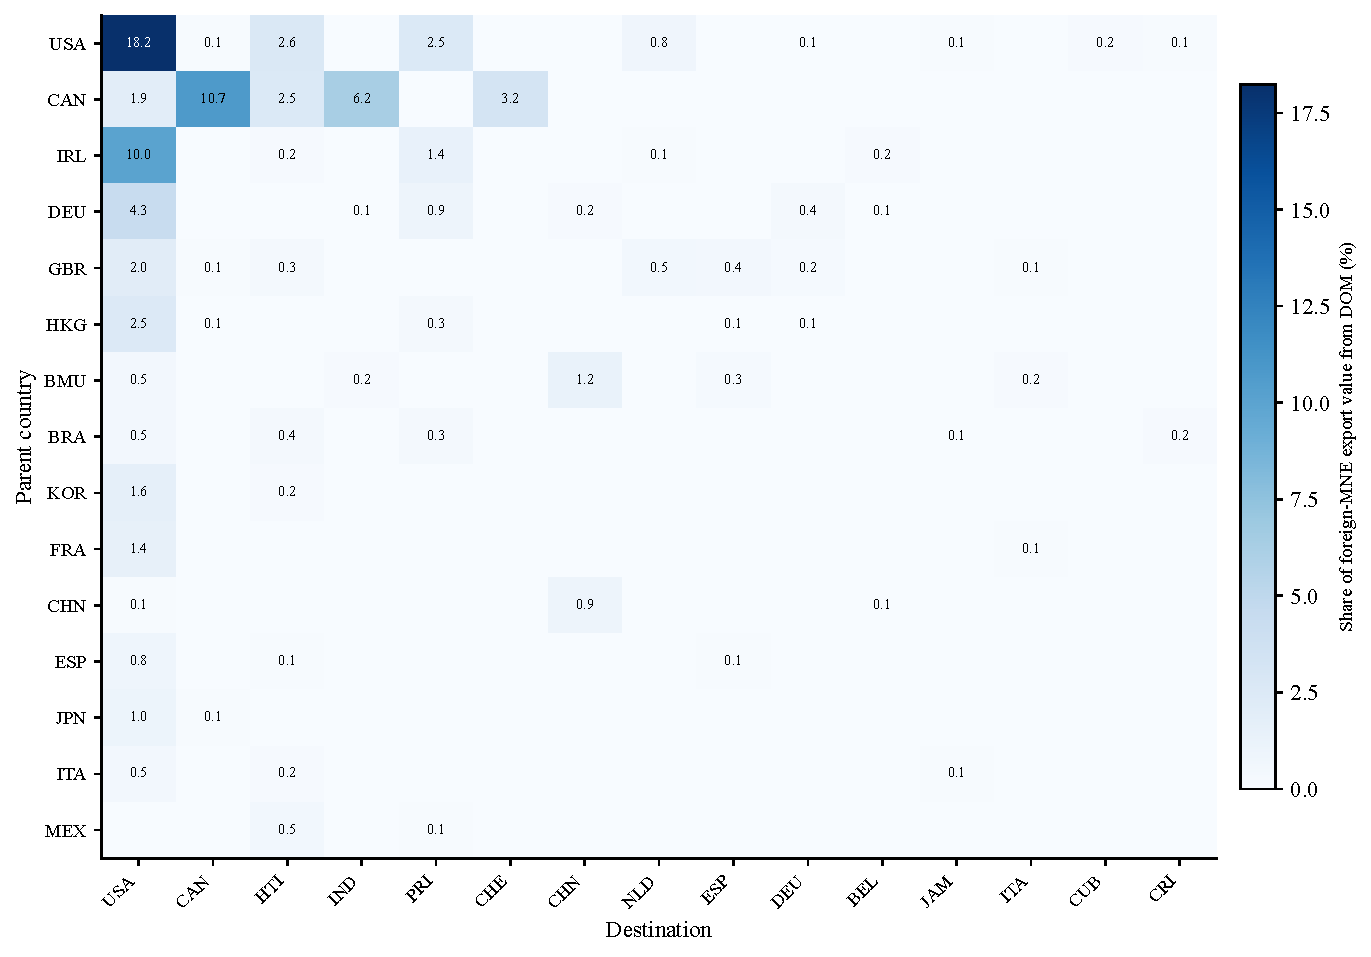
\includegraphics[width=1.0\textwidth,height=0.8\textheight,keepaspectratio]{figures/all/fig_wp1d_heatmap_country_cellpct_DOM.pdf}%
  \caption{Dominican Republic: Foreign-Multinational Exports by Parent Country and Destination}%
  \label{fig:c_hm_DOM}%
  \par\vspace{2pt}%
  \parbox{0.92\textwidth}{\footnotesize %
  \textit{Notes:} Percent of the foreign-MNE export value of Dominican Republic in each parent country and destination pair; fifteen largest parent countries and destinations.\\[3pt]%
  \textit{Source:} Authors' calculations based on customs data matched to Orbis and Dun \& Bradstreet.}%
  \end{figure}
% ---- Figure: Dominican Republic: Share of Foreign-Multinational Exports Shipped to the Parent Country
\begin{figure}[H]\centering%
  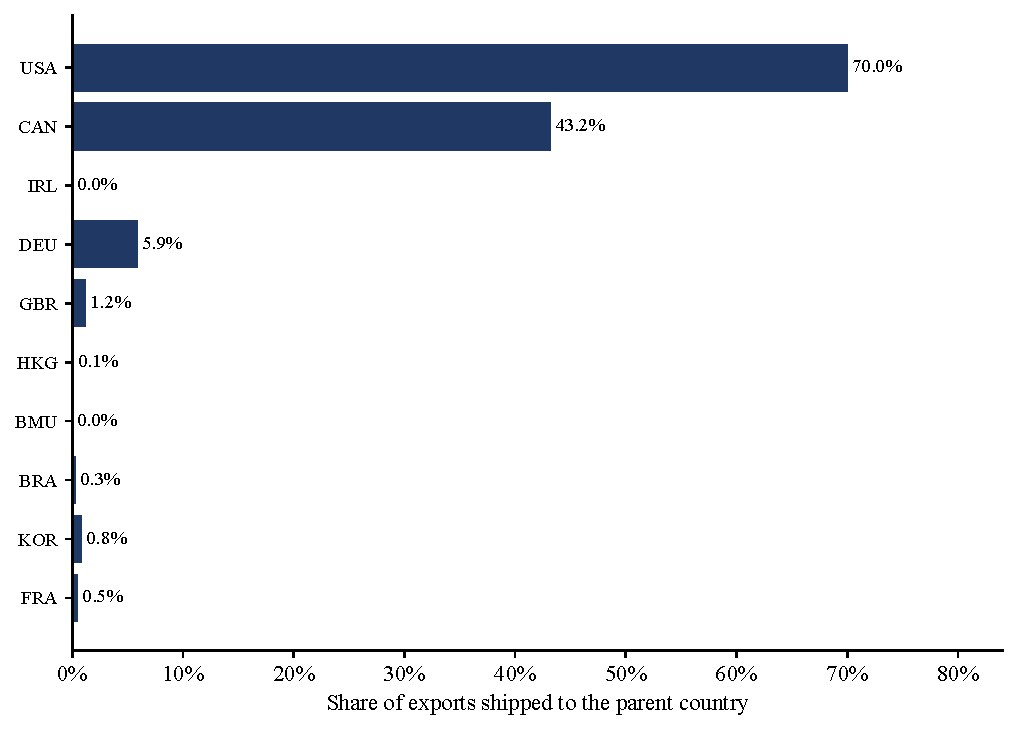
\includegraphics[width=0.85\textwidth,height=0.8\textheight,keepaspectratio]{figures/all/fig_wp1d_home_share_by_parent_DOM.pdf}%
  \caption{Dominican Republic: Share of Foreign-Multinational Exports Shipped to the Parent Country}%
  \label{fig:c_home_DOM}%
  \par\vspace{2pt}%
  \parbox{0.92\textwidth}{\footnotesize %
  \textit{Notes:} Percent of each parent country's exports from Dominican Republic shipped to that same country; ten largest parent countries.\\[3pt]%
  \textit{Source:} Authors' calculations based on customs data matched to Orbis and Dun \& Bradstreet.}%
  \end{figure}
% ---- Table: Dominican Republic, Agriculture: Multinational Exports by Parent Region and Destination Region
\begin{table}[H]\centering\small%
  \caption{Dominican Republic, Agriculture: Multinational Exports by Parent Region and Destination Region}%
  \label{tab:c_reg_DOM_agro}%
  \adjustbox{max width=\textwidth, max totalheight=0.8\textheight}{\begin{tabular}{lrrrrrrrr}
\toprule
DOM: parent region \ destination & Latin America & North America & Europe & Asia & Africa & Oceania & Rest of World & Total \\
\midrule
Latin America & 73.5 & 21.3 & 3.9 & 1.0 & 0.3 & 0.0 & 0.0 & 0.1 \\
North America & 22.1 & 68.2 & 9.1 & 0.1 & 0.2 & 0.0 & 0.3 & 0.2 \\
Europe & 22.1 & 46.2 & 29.2 & 1.6 & 0.1 & 0.0 & 0.9 & 0.3 \\
Asia & 9.2 & 81.7 & 5.0 & 4.1 & 0.0 & 0.0 & 0.0 & 0.3 \\
Africa & 85.4 & 4.2 & 8.9 & 1.3 & 0.1 & 0.1 & 0.0 & 0.0 \\
Oceania & 100.0 & 0.0 & 0.0 & 0.0 & 0.0 & 0.0 & 0.0 & 0.0 \\
Domestic MNEs & 8.9 & 79.4 & 10.3 & 0.0 & 0.0 & 0.0 & 1.4 & 0.1 \\
Local firms & 25.6 & 38.8 & 33.3 & 1.7 & 0.1 & 0.0 & 0.5 & 1.1 \\
\bottomrule
\end{tabular}
}%
  \par\vspace{3pt}%
  \begin{minipage}{0.95\textwidth}\footnotesize %
  \textit{Notes:} Percent of each group's agricultural exports from Dominican Republic, by destination region (rows add to 100). Last column: the group's exports. Values are annual averages in US\$ billion.\\[3pt]%
  \textit{Source:} Authors' calculations based on customs data matched to Orbis and Dun \& Bradstreet.%
  \end{minipage}%
  \end{table}
% ---- Table: Dominican Republic, Manufacturing: Multinational Exports by Parent Region and Destination Region
\begin{table}[H]\centering\small%
  \caption{Dominican Republic, Manufacturing: Multinational Exports by Parent Region and Destination Region}%
  \label{tab:c_reg_DOM_manufacturing}%
  \adjustbox{max width=\textwidth, max totalheight=0.8\textheight}{\begin{tabular}{lrrrrrrrr}
\toprule
DOM: parent region \ destination & Latin America & North America & Europe & Asia & Africa & Oceania & Rest of World & Total \\
\midrule
Latin America & 36.7 & 21.9 & 10.8 & 27.5 & 2.0 & 0.0 & 1.1 & 0.4 \\
North America & 32.5 & 61.7 & 3.3 & 2.1 & 0.0 & 0.4 & 0.0 & 1.4 \\
Europe & 15.8 & 71.0 & 9.4 & 3.5 & 0.0 & 0.3 & 0.0 & 1.3 \\
Asia & 14.6 & 81.4 & 0.9 & 3.1 & 0.0 & 0.0 & 0.0 & 0.1 \\
Africa & 31.7 & 55.9 & 2.0 & 9.6 & 0.7 & 0.0 & 0.0 & 0.0 \\
Oceania & 0.7 & 26.0 & 42.6 & 4.6 & 4.1 & 22.0 & 0.0 & 0.0 \\
Rest of World & 100.0 & 0.0 & 0.0 & 0.0 & 0.0 & 0.0 & 0.0 & 0.0 \\
Domestic MNEs & 40.4 & 20.9 & 36.9 & 0.3 & 0.0 & 1.5 & 0.0 & 0.0 \\
Local firms & 36.4 & 51.8 & 3.1 & 8.4 & 0.1 & 0.1 & 0.2 & 1.2 \\
\bottomrule
\end{tabular}
}%
  \par\vspace{3pt}%
  \begin{minipage}{0.95\textwidth}\footnotesize %
  \textit{Notes:} Percent of each group's manufacturing exports from Dominican Republic, by destination region (rows add to 100). Last column: the group's exports. Values are annual averages in US\$ billion.\\[3pt]%
  \textit{Source:} Authors' calculations based on customs data matched to Orbis and Dun \& Bradstreet.%
  \end{minipage}%
  \end{table}
% ---- Table: Dominican Republic, Mining and Fuels: Multinational Exports by Parent Region and Destination Region
\begin{table}[H]\centering\small%
  \caption{Dominican Republic, Mining and Fuels: Multinational Exports by Parent Region and Destination Region}%
  \label{tab:c_reg_DOM_mining}%
  \adjustbox{max width=\textwidth, max totalheight=0.8\textheight}{\begin{tabular}{lrrrrrrrr}
\toprule
DOM: parent region \ destination & Latin America & North America & Europe & Asia & Africa & Oceania & Rest of World & Total \\
\midrule
Latin America & 76.1 & 23.5 & 0.1 & 0.0 & 0.0 & 0.0 & 0.3 & 0.1 \\
North America & 0.2 & 59.1 & 13.8 & 26.9 & 0.0 & 0.0 & 0.0 & 1.3 \\
Europe & 14.1 & 80.7 & 0.1 & 4.8 & 0.0 & 0.0 & 0.3 & 0.2 \\
Asia & 0.1 & 5.1 & 5.2 & 89.7 & 0.0 & 0.0 & 0.0 & 0.1 \\
Africa & 5.0 & 18.9 & 4.4 & 0.0 & 71.6 & 0.0 & 0.0 & 0.0 \\
Oceania & 0.0 & 1.3 & 98.7 & 0.0 & 0.0 & 0.0 & 0.0 & 0.0 \\
Domestic MNEs & 89.3 & 0.0 & 0.0 & 0.0 & 0.0 & 0.0 & 10.7 & 0.0 \\
Local firms & 36.7 & 56.6 & 2.1 & 0.0 & 4.5 & 0.0 & 0.0 & 0.3 \\
\bottomrule
\end{tabular}
}%
  \par\vspace{3pt}%
  \begin{minipage}{0.95\textwidth}\footnotesize %
  \textit{Notes:} Percent of each group's mining and fuels exports from Dominican Republic, by destination region (rows add to 100). Last column: the group's exports. Values are annual averages in US\$ billion.\\[3pt]%
  \textit{Source:} Authors' calculations based on customs data matched to Orbis and Dun \& Bradstreet.%
  \end{minipage}%
  \end{table}

\subsection{Products}
% ---- Table: Dominican Republic: Fifteen Largest Export Products
\begin{table}[H]\centering\footnotesize%
  \caption{Dominican Republic: Fifteen Largest Export Products}%
  \label{tab:c_hs6_DOM}%
  \adjustbox{max width=\textwidth, max totalheight=0.8\textheight}{\begin{tabular}{@{}l p{6.4cm} r r r r l@{}}
\toprule
HS6 & Description & US\$bn/yr & Foreign (\%) & Domestic (\%) & Local (\%) & Leading parent \\
\midrule
710812 & Gold (incl. gold plated with platinum), in unwrought forms (excl. powder) & 1.25 & 100 & 0 & 0 & CAN (0.97) \\
901890 & Instruments and appliances used in medical/\allowbreak{}surgical/\allowbreak{}veterinary sciences, incl. other electro-m... & 0.74 & 100 & 0 & 0 & DEU (0.43) \\
240210 & Cigars, cheroots and cigarillos containing tobacco & 0.62 & 62 & 0 & 38 & HKG (0.40) \\
853620 & Automatic circuit breakers, for a voltage not >1000V & 0.43 & 100 & 0 & 0 & IRL (0.92) \\
610910 & T-shirts, singlets and other vests, knitted/\allowbreak{}crocheted, of cotton & 0.29 & 65 & 0 & 35 & CAN (0.44) \\
711319 & Articles of jewellery and parts thereof , of other precious metal (excl. silver), whether/\allowbreak{}not ... & 0.28 & 56 & 0 & 44 & USA (0.39) \\
080300 & Bananas, incl. plantains, fresh/\allowbreak{}dried & 0.21 & 8 & 0 & 92 & USA (0.34) \\
300691 & Appliances identifiable for ostomy use & 0.19 & 100 & 0 & 0 & GBR (0.80) \\
180100 & Cocoa beans, whole/\allowbreak{}broken, raw/\allowbreak{}roasted & 0.19 & 6 & 0 & 94 & CHE (0.95) \\
720260 & Ferro-nickel, in granular/\allowbreak{}powder form & 0.16 & 100 & 0 & 0 & BMU (1.00) \\
640510 & Footwear with uppers of leather/\allowbreak{}composition leather, n.e.s. & 0.15 & 77 & 0 & 23 & USA (0.99) \\
521213 & Woven fabrics of cotton (excl. of 52.08-52.11), dyed, weighing not >200 g/\allowbreak{}m2 & 0.13 & 97 & 0 & 3 & USA (1.00) \\
300610 & Sterile surgical catgut, similar sterile suture materials (including sterile absorbable surgic... & 0.13 & 100 & 0 & 0 & IRL (1.00) \\
170111 & Cane sugar, raw, in solid form, not containing added flavouring/\allowbreak{}colouring matter & 0.10 & 25 & 62 & 13 & LIE (1.00) \\
640399 & Other footwear without  outer soles of  leather, not covering the ankle. & 0.10 & 51 & 0 & 49 & BRA (0.55) \\
\bottomrule
\end{tabular}
}%
  \par\vspace{3pt}%
  \begin{minipage}{0.95\textwidth}\footnotesize %
  \textit{Notes:} Fifteen largest HS6 products exported by Dominican Republic. Foreign, domestic and local: percent of the product's export value. Leading parent: largest parent country and its share of the product's foreign-MNE exports. Values are annual averages in US\$ billion.\\[3pt]%
  \textit{Source:} Authors' calculations based on customs data matched to Orbis and Dun \& Bradstreet.%
  \end{minipage}%
  \end{table}
% ---- Table: Dominican Republic, Agriculture: Fifteen Largest Export Products
\begin{table}[H]\centering\footnotesize%
  \caption{Dominican Republic, Agriculture: Fifteen Largest Export Products}%
  \label{tab:c_hs6_DOM_agro}%
  \adjustbox{max width=\textwidth, max totalheight=0.8\textheight}{\begin{tabular}{@{}l p{6.4cm} r r r r l@{}}
\toprule
HS6 & Description & US\$bn/yr & Foreign (\%) & Domestic (\%) & Local (\%) & Leading parent \\
\midrule
240210 & Cigars, cheroots and cigarillos containing tobacco & 0.62 & 62 & 0 & 38 & HKG (0.40) \\
080300 & Bananas, incl. plantains, fresh/\allowbreak{}dried & 0.21 & 8 & 0 & 92 & USA (0.34) \\
180100 & Cocoa beans, whole/\allowbreak{}broken, raw/\allowbreak{}roasted & 0.19 & 6 & 0 & 94 & CHE (0.95) \\
170111 & Cane sugar, raw, in solid form, not containing added flavouring/\allowbreak{}colouring matter & 0.10 & 25 & 62 & 13 & LIE (1.00) \\
220840 & Rum and tafia & 0.08 & 74 & 0 & 26 & GBR (0.78) \\
210390 & Sauces and preparations therefor, n.e.s.; mixed condiments and mixed seasonings, n.e.s. & 0.06 & 71 & 0 & 29 & COL (0.44) \\
240120 & Tobacco, partly/\allowbreak{}wholly stemmed/\allowbreak{}stripped & 0.04 & 82 & 0 & 18 & HKG (0.79) \\
210690 & Food preparations, n.e.s. & 0.04 & 53 & 0 & 47 & CHL (0.87) \\
110100 & Wheat/\allowbreak{}meslin flour & 0.04 & 77 & 0 & 23 & GTM (1.00) \\
080440 & Avocados, fresh/\allowbreak{}dried & 0.03 & 12 & 0 & 88 & ESP (0.91) \\
240110 & Tobacco, not stemmed/\allowbreak{}stripped & 0.03 & 60 & 0 & 40 & DNK (0.49) \\
240391 & Homogenised/\allowbreak{}reconstituted tobacco & 0.03 & 91 & 0 & 9 & LVA (0.98) \\
220300 & Beer made from malt & 0.02 & 98 & 0 & 2 & LUX (1.00) \\
190531 & Sweet biscuits & 0.02 & 1 & 0 & 99 & MKD (0.32) \\
070960 & Fruits of the genera Capsicum/\allowbreak{}Pimenta, fresh/\allowbreak{}chilled & 0.02 & 11 & 0 & 89 & CAN (0.26) \\
\bottomrule
\end{tabular}
}%
  \par\vspace{3pt}%
  \begin{minipage}{0.95\textwidth}\footnotesize %
  \textit{Notes:} Fifteen largest agricultural HS6 products exported by Dominican Republic. Foreign, domestic and local: percent of the product's export value. Leading parent: largest parent country and its share of the product's foreign-MNE exports. Values are annual averages in US\$ billion.\\[3pt]%
  \textit{Source:} Authors' calculations based on customs data matched to Orbis and Dun \& Bradstreet.%
  \end{minipage}%
  \end{table}
% ---- Table: Dominican Republic, Manufacturing: Fifteen Largest Export Products
\begin{table}[H]\centering\footnotesize%
  \caption{Dominican Republic, Manufacturing: Fifteen Largest Export Products}%
  \label{tab:c_hs6_DOM_manufacturing}%
  \adjustbox{max width=\textwidth, max totalheight=0.8\textheight}{\begin{tabular}{@{}l p{6.4cm} r r r r l@{}}
\toprule
HS6 & Description & US\$bn/yr & Foreign (\%) & Domestic (\%) & Local (\%) & Leading parent \\
\midrule
901890 & Instruments and appliances used in medical/\allowbreak{}surgical/\allowbreak{}veterinary sciences, incl. other electro-m... & 0.74 & 100 & 0 & 0 & DEU (0.43) \\
853620 & Automatic circuit breakers, for a voltage not >1000V & 0.43 & 100 & 0 & 0 & IRL (0.92) \\
610910 & T-shirts, singlets and other vests, knitted/\allowbreak{}crocheted, of cotton & 0.29 & 65 & 0 & 35 & CAN (0.44) \\
300691 & Appliances identifiable for ostomy use & 0.19 & 100 & 0 & 0 & GBR (0.80) \\
720260 & Ferro-nickel, in granular/\allowbreak{}powder form & 0.16 & 100 & 0 & 0 & BMU (1.00) \\
640510 & Footwear with uppers of leather/\allowbreak{}composition leather, n.e.s. & 0.15 & 77 & 0 & 23 & USA (0.99) \\
521213 & Woven fabrics of cotton (excl. of 52.08-52.11), dyed, weighing not >200 g/\allowbreak{}m2 & 0.13 & 97 & 0 & 3 & USA (1.00) \\
300610 & Sterile surgical catgut, similar sterile suture materials (including sterile absorbable surgic... & 0.13 & 100 & 0 & 0 & IRL (1.00) \\
640399 & Other footwear without  outer soles of  leather, not covering the ankle. & 0.10 & 51 & 0 & 49 & BRA (0.55) \\
851712 & Telephones for cellular networks/\allowbreak{}for other wireless networks, other than Line telephone sets w... & 0.06 & 1 & 0 & 99 & MEX (0.41) \\
620342 & Men's/\allowbreak{}boys' trousers, bib and brace overalls, breeches and shorts (excl. swimwear; excl. knitt... & 0.06 & 9 & 0 & 91 & TUN (0.96) \\
621210 & BrassiFres and parts thereof , whether/\allowbreak{}not knitted/\allowbreak{}crocheted & 0.06 & 98 & 0 & 2 & USA (0.58) \\
630790 & Other made-up textile articles, incl. dress patterns, n.e.s. & 0.05 & 99 & 0 & 1 & USA (1.00) \\
901839 & Catheters, cannulae and the like & 0.05 & 97 & 0 & 3 & USA (0.98) \\
721420 & Bars and rods of iron/\allowbreak{}non-alloy steel (excl. of 72,13), containing indentations/\allowbreak{}ribs/\allowbreak{}grooves/\allowbreak{}o... & 0.05 & 80 & 0 & 20 & BRA (0.84) \\
\bottomrule
\end{tabular}
}%
  \par\vspace{3pt}%
  \begin{minipage}{0.95\textwidth}\footnotesize %
  \textit{Notes:} Fifteen largest manufacturing HS6 products exported by Dominican Republic. Foreign, domestic and local: percent of the product's export value. Leading parent: largest parent country and its share of the product's foreign-MNE exports. Values are annual averages in US\$ billion.\\[3pt]%
  \textit{Source:} Authors' calculations based on customs data matched to Orbis and Dun \& Bradstreet.%
  \end{minipage}%
  \end{table}
% ---- Table: Dominican Republic, Mining and Fuels: Fifteen Largest Export Products
\begin{table}[H]\centering\footnotesize%
  \caption{Dominican Republic, Mining and Fuels: Fifteen Largest Export Products}%
  \label{tab:c_hs6_DOM_mining}%
  \adjustbox{max width=\textwidth, max totalheight=0.8\textheight}{\begin{tabular}{@{}l p{6.4cm} r r r r l@{}}
\toprule
HS6 & Description & US\$bn/yr & Foreign (\%) & Domestic (\%) & Local (\%) & Leading parent \\
\midrule
710812 & Gold (incl. gold plated with platinum), in unwrought forms (excl. powder) & 1.25 & 100 & 0 & 0 & CAN (0.97) \\
711319 & Articles of jewellery and parts thereof , of other precious metal (excl. silver), whether/\allowbreak{}not ... & 0.28 & 56 & 0 & 44 & USA (0.39) \\
271011 & Light petroleum oils and preparations & 0.09 & 7 & 0 & 93 & FRA (0.63) \\
252329 & Portland cement (excl. white cement, whether/\allowbreak{}not artificially coloured), whether/\allowbreak{}not coloured & 0.08 & 72 & 0 & 28 & MEX (0.51) \\
710813 & Gold (incl. gold plated with platinum), non-monetary, in semi-manufactured forms & 0.07 & 82 & 0 & 18 & ESP (0.71) \\
260300 & Copper ores and concentrates & 0.06 & 100 & 0 & 0 & CHN (0.97) \\
711311 & Articles of jewellery and parts thereof , of silver, whether/\allowbreak{}not plated/\allowbreak{}clad with other precio... & 0.05 & 70 & 0 & 30 & FRA (0.50) \\
711291 & Waste and scrap of gold, incl. metal clad with gold but excl. sweepings containing other preci... & 0.01 & 43 & 0 & 57 & USA (0.92) \\
710691 & Silver (incl. silver plated with gold/\allowbreak{}platinum), unwrought & 0.01 & 98 & 0 & 2 & AUS (0.95) \\
260600 & Aluminium ores and concentrates & 0.01 & 100 & 0 & 0 & CYP (1.00) \\
711011 & Platinum, unwrought/\allowbreak{}in powder form & 0.01 & 100 & 0 & 0 & FRA (0.99) \\
260800 & Zinc ores and concentrates & 0.01 & 100 & 0 & 0 & CHN (1.00) \\
252310 & Cement clinkers & 0.00 & 77 & 0 & 23 & ITA (0.49) \\
711299 & Waste and scrap of precious metal/\allowbreak{}of metal clad with precious metal; other waste and scrap con... & 0.00 & 7 & 0 & 93 & CHN (0.44) \\
271111 & Natural gas, liquefied & 0.00 & 99 & 0 & 1 & USA (0.86) \\
\bottomrule
\end{tabular}
}%
  \par\vspace{3pt}%
  \begin{minipage}{0.95\textwidth}\footnotesize %
  \textit{Notes:} Fifteen largest mining and fuels HS6 products exported by Dominican Republic. Foreign, domestic and local: percent of the product's export value. Leading parent: largest parent country and its share of the product's foreign-MNE exports. Values are annual averages in US\$ billion.\\[3pt]%
  \textit{Source:} Authors' calculations based on customs data matched to Orbis and Dun \& Bradstreet.%
  \end{minipage}%
  \end{table}

\section{Peru}\label{sec:c_PER}

\subsection{Parents and Destinations}
% ---- Table: Peru: Multinational Exports by Parent Region and Destination Region
\begin{table}[H]\centering\small%
  \caption{Peru: Multinational Exports by Parent Region and Destination Region}%
  \label{tab:c_reg_PER}%
  \adjustbox{max width=\textwidth, max totalheight=0.8\textheight}{\begin{tabular}{lrrrrrrrr}
\toprule
PER: parent region \ destination & Latin America & North America & Europe & Asia & Africa & Oceania & Rest of World & Total \\
\midrule
Latin America & 19.3 & 14.9 & 25.4 & 38.2 & 0.8 & 1.4 & 0.0 & 3.3 \\
North America & 8.3 & 8.6 & 35.2 & 47.8 & 0.0 & 0.1 & 0.0 & 4.7 \\
Europe & 12.5 & 12.1 & 21.6 & 51.3 & 2.2 & 0.4 & 0.0 & 6.7 \\
Asia & 48.8 & 19.9 & 8.3 & 22.7 & 0.2 & 0.1 & 0.0 & 0.3 \\
Africa & 1.6 & 3.9 & 35.9 & 57.2 & 1.3 & 0.0 & 0.0 & 0.4 \\
Oceania & 17.3 & 1.5 & 3.9 & 77.2 & 0.0 & 0.0 & 0.0 & 0.9 \\
Rest of World & 9.0 & 36.2 & 28.7 & 15.5 & 0.0 & 10.5 & 0.0 & 0.0 \\
Domestic MNEs & 38.5 & 30.4 & 12.6 & 14.4 & 3.7 & 0.4 & 0.0 & 1.0 \\
Local firms & 18.3 & 28.0 & 24.6 & 28.1 & 0.3 & 0.4 & 0.2 & 22.1 \\
\bottomrule
\end{tabular}
}%
  \par\vspace{3pt}%
  \begin{minipage}{0.95\textwidth}\footnotesize %
  \textit{Notes:} Percent of each group's exports from Peru, by destination region (rows add to 100). Last column: the group's exports. Values are annual averages in US\$ billion.\\[3pt]%
  \textit{Source:} Authors' calculations based on customs data matched to Orbis and Dun \& Bradstreet.%
  \end{minipage}%
  \end{table}
% ---- Figure: Peru: Foreign-Multinational Exports by Parent Country and Destination
\begin{figure}[H]\centering%
  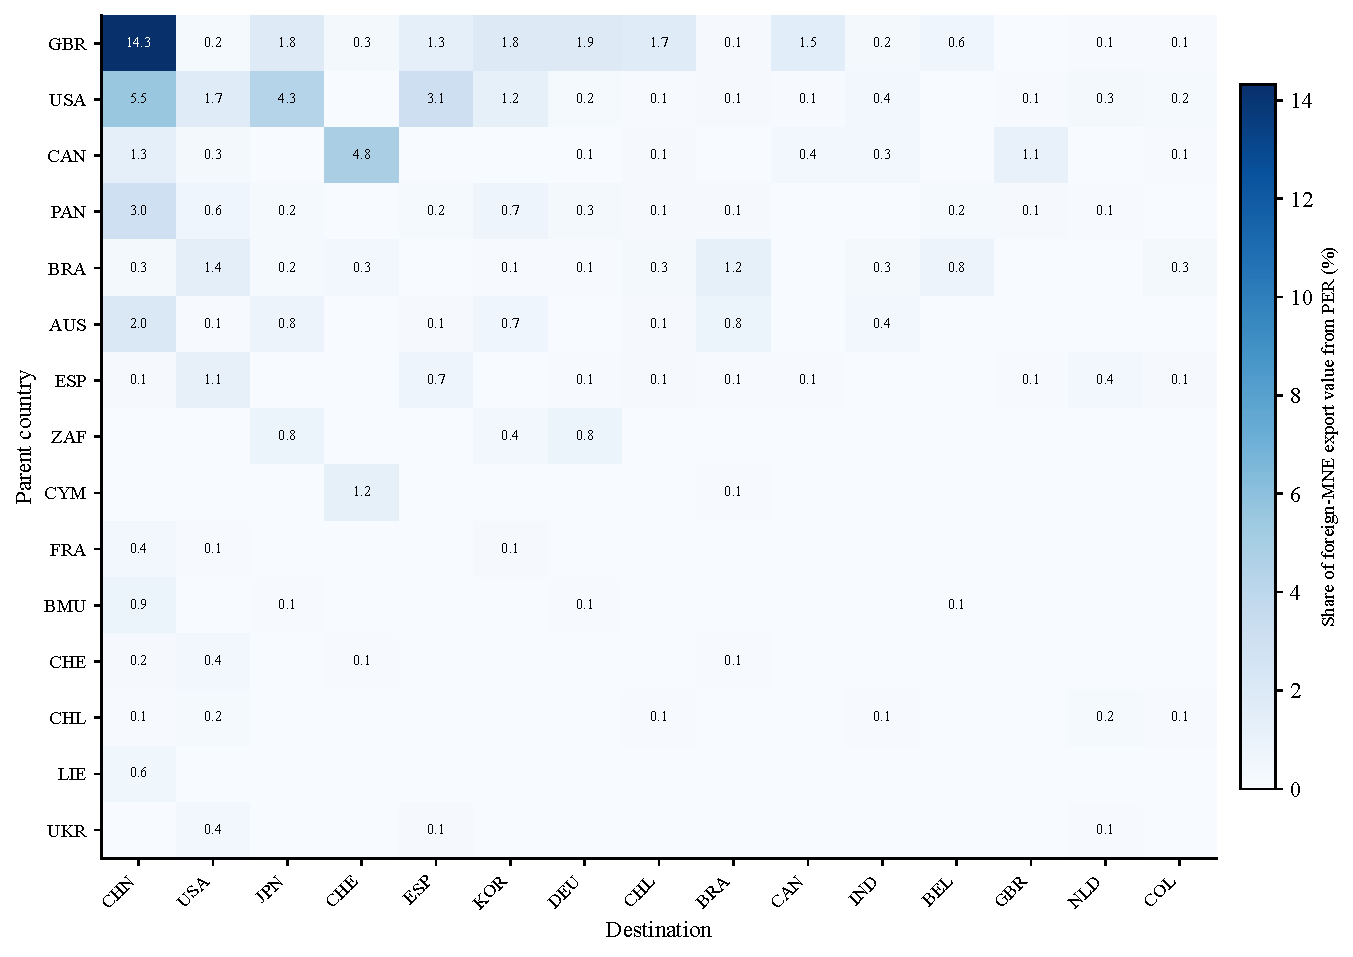
\includegraphics[width=1.0\textwidth,height=0.8\textheight,keepaspectratio]{figures/all/fig_wp1d_heatmap_country_cellpct_PER.pdf}%
  \caption{Peru: Foreign-Multinational Exports by Parent Country and Destination}%
  \label{fig:c_hm_PER}%
  \par\vspace{2pt}%
  \parbox{0.92\textwidth}{\footnotesize %
  \textit{Notes:} Percent of the foreign-MNE export value of Peru in each parent country and destination pair; fifteen largest parent countries and destinations.\\[3pt]%
  \textit{Source:} Authors' calculations based on customs data matched to Orbis and Dun \& Bradstreet.}%
  \end{figure}
% ---- Figure: Peru: Share of Foreign-Multinational Exports Shipped to the Parent Country
\begin{figure}[H]\centering%
  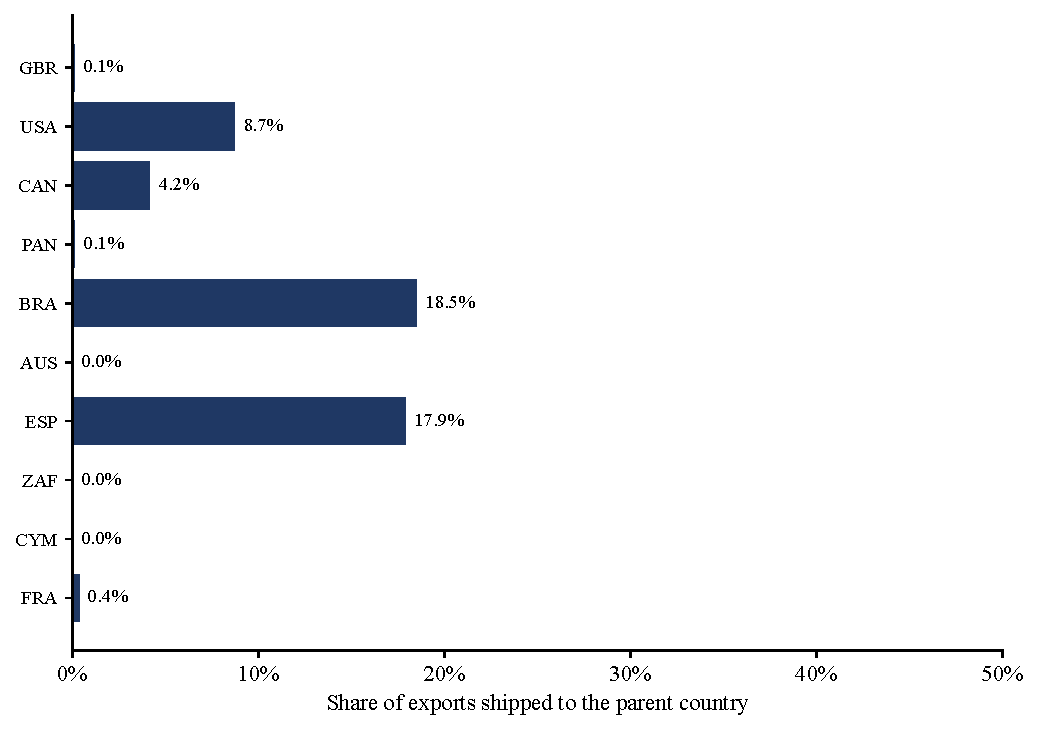
\includegraphics[width=0.85\textwidth,height=0.8\textheight,keepaspectratio]{figures/all/fig_wp1d_home_share_by_parent_PER.pdf}%
  \caption{Peru: Share of Foreign-Multinational Exports Shipped to the Parent Country}%
  \label{fig:c_home_PER}%
  \par\vspace{2pt}%
  \parbox{0.92\textwidth}{\footnotesize %
  \textit{Notes:} Percent of each parent country's exports from Peru shipped to that same country; ten largest parent countries.\\[3pt]%
  \textit{Source:} Authors' calculations based on customs data matched to Orbis and Dun \& Bradstreet.}%
  \end{figure}
% ---- Table: Peru, Agriculture: Multinational Exports by Parent Region and Destination Region
\begin{table}[H]\centering\small%
  \caption{Peru, Agriculture: Multinational Exports by Parent Region and Destination Region}%
  \label{tab:c_reg_PER_agro}%
  \adjustbox{max width=\textwidth, max totalheight=0.8\textheight}{\begin{tabular}{lrrrrrrrr}
\toprule
PER: parent region \ destination & Latin America & North America & Europe & Asia & Africa & Oceania & Rest of World & Total \\
\midrule
Latin America & 7.7 & 19.6 & 26.9 & 44.3 & 0.6 & 0.8 & 0.0 & 0.8 \\
North America & 78.2 & 10.0 & 6.4 & 5.4 & 0.0 & 0.0 & 0.0 & 0.2 \\
Europe & 13.5 & 28.1 & 37.7 & 18.4 & 1.7 & 0.5 & 0.0 & 1.0 \\
Asia & 19.1 & 30.6 & 27.1 & 22.8 & 0.3 & 0.1 & 0.0 & 0.1 \\
Africa & 5.4 & 31.4 & 47.1 & 15.1 & 0.4 & 0.7 & 0.0 & 0.0 \\
Oceania & 0.0 & 90.7 & 9.0 & 0.3 & 0.0 & 0.0 & 0.0 & 0.0 \\
Rest of World & 7.3 & 41.5 & 32.9 & 17.5 & 0.0 & 0.8 & 0.0 & 0.0 \\
Domestic MNEs & 14.8 & 16.3 & 28.5 & 38.4 & 0.9 & 1.0 & 0.0 & 0.4 \\
Local firms & 13.7 & 25.8 & 35.5 & 23.4 & 0.5 & 1.0 & 0.0 & 5.0 \\
\bottomrule
\end{tabular}
}%
  \par\vspace{3pt}%
  \begin{minipage}{0.95\textwidth}\footnotesize %
  \textit{Notes:} Percent of each group's agricultural exports from Peru, by destination region (rows add to 100). Last column: the group's exports. Values are annual averages in US\$ billion.\\[3pt]%
  \textit{Source:} Authors' calculations based on customs data matched to Orbis and Dun \& Bradstreet.%
  \end{minipage}%
  \end{table}
% ---- Table: Peru, Manufacturing: Multinational Exports by Parent Region and Destination Region
\begin{table}[H]\centering\small%
  \caption{Peru, Manufacturing: Multinational Exports by Parent Region and Destination Region}%
  \label{tab:c_reg_PER_manufacturing}%
  \adjustbox{max width=\textwidth, max totalheight=0.8\textheight}{\begin{tabular}{lrrrrrrrr}
\toprule
PER: parent region \ destination & Latin America & North America & Europe & Asia & Africa & Oceania & Rest of World & Total \\
\midrule
Latin America & 37.2 & 21.2 & 20.0 & 19.2 & 2.4 & 0.0 & 0.0 & 0.9 \\
North America & 24.1 & 31.5 & 18.1 & 26.1 & 0.1 & 0.1 & 0.0 & 0.3 \\
Europe & 51.1 & 17.9 & 16.9 & 13.4 & 0.2 & 0.5 & 0.0 & 0.5 \\
Asia & 85.6 & 8.8 & 3.9 & 1.3 & 0.3 & 0.1 & 0.0 & 0.2 \\
Africa & 74.3 & 16.1 & 6.0 & 3.0 & 0.6 & 0.0 & 0.1 & 0.0 \\
Oceania & 1.8 & 75.2 & 9.7 & 13.4 & 0.0 & 0.0 & 0.0 & 0.0 \\
Rest of World & 20.4 & 0.6 & 0.1 & 2.1 & 0.0 & 76.5 & 0.2 & 0.0 \\
Domestic MNEs & 89.3 & 8.8 & 0.8 & 0.7 & 0.1 & 0.2 & 0.0 & 0.4 \\
Local firms & 40.4 & 19.7 & 16.0 & 23.1 & 0.3 & 0.4 & 0.0 & 5.3 \\
\bottomrule
\end{tabular}
}%
  \par\vspace{3pt}%
  \begin{minipage}{0.95\textwidth}\footnotesize %
  \textit{Notes:} Percent of each group's manufacturing exports from Peru, by destination region (rows add to 100). Last column: the group's exports. Values are annual averages in US\$ billion.\\[3pt]%
  \textit{Source:} Authors' calculations based on customs data matched to Orbis and Dun \& Bradstreet.%
  \end{minipage}%
  \end{table}
% ---- Table: Peru, Mining and Fuels: Multinational Exports by Parent Region and Destination Region
\begin{table}[H]\centering\small%
  \caption{Peru, Mining and Fuels: Multinational Exports by Parent Region and Destination Region}%
  \label{tab:c_reg_PER_mining}%
  \adjustbox{max width=\textwidth, max totalheight=0.8\textheight}{\begin{tabular}{lrrrrrrrr}
\toprule
PER: parent region \ destination & Latin America & North America & Europe & Asia & Africa & Oceania & Rest of World & Total \\
\midrule
Latin America & 15.0 & 9.3 & 27.5 & 45.7 & 0.0 & 2.5 & 0.0 & 1.6 \\
North America & 4.0 & 6.8 & 37.8 & 51.3 & 0.0 & 0.1 & 0.0 & 4.2 \\
Europe & 8.5 & 8.3 & 18.8 & 61.5 & 2.5 & 0.3 & 0.0 & 5.2 \\
Asia & 9.8 & 30.4 & 0.9 & 58.9 & 0.0 & 0.0 & 0.0 & 0.1 \\
Africa & 0.7 & 2.9 & 35.9 & 59.1 & 1.4 & 0.0 & 0.0 & 0.4 \\
Oceania & 17.6 & 0.3 & 3.8 & 78.3 & 0.0 & 0.0 & 0.0 & 0.9 \\
Domestic MNEs & 1.4 & 78.6 & 7.1 & 0.7 & 12.2 & 0.0 & 0.0 & 0.3 \\
Local firms & 10.3 & 32.7 & 23.8 & 32.4 & 0.2 & 0.1 & 0.5 & 11.8 \\
\bottomrule
\end{tabular}
}%
  \par\vspace{3pt}%
  \begin{minipage}{0.95\textwidth}\footnotesize %
  \textit{Notes:} Percent of each group's mining and fuels exports from Peru, by destination region (rows add to 100). Last column: the group's exports. Values are annual averages in US\$ billion.\\[3pt]%
  \textit{Source:} Authors' calculations based on customs data matched to Orbis and Dun \& Bradstreet.%
  \end{minipage}%
  \end{table}
% ---- Table: Peru, Other Goods: Multinational Exports by Parent Region and Destination Region
\begin{table}[H]\centering\small%
  \caption{Peru, Other Goods: Multinational Exports by Parent Region and Destination Region}%
  \label{tab:c_reg_PER_rest}%
  \adjustbox{max width=\textwidth, max totalheight=0.8\textheight}{\begin{tabular}{lrrrrrrr}
\toprule
PER: parent region \ destination & Latin America & North America & Europe & Asia & Africa & Oceania & Total \\
\midrule
Latin America & 63.9 & 8.4 & 4.3 & 23.4 & 0.0 & 0.0 & 0.0 \\
North America & 8.1 & 91.9 & 0.0 & 0.0 & 0.0 & 0.0 & 0.0 \\
Europe & 82.5 & 4.8 & 9.3 & 3.4 & 0.0 & 0.0 & 0.0 \\
Asia & 52.5 & 28.9 & 0.2 & 18.4 & 0.0 & 0.0 & 0.0 \\
Africa & 0.0 & 100.0 & 0.0 & 0.0 & 0.0 & 0.0 & 0.0 \\
Domestic MNEs & 92.3 & 6.1 & 1.6 & 0.0 & 0.0 & 0.0 & 0.0 \\
Local firms & 48.5 & 24.9 & 17.9 & 7.0 & 0.2 & 1.5 & 0.0 \\
\bottomrule
\end{tabular}
}%
  \par\vspace{3pt}%
  \begin{minipage}{0.95\textwidth}\footnotesize %
  \textit{Notes:} Percent of each group's exports from Peru, by destination region (rows add to 100). Last column: the group's exports. Values are annual averages in US\$ billion.\\[3pt]%
  \textit{Source:} Authors' calculations based on customs data matched to Orbis and Dun \& Bradstreet.%
  \end{minipage}%
  \end{table}

\subsection{Products}
% ---- Table: Peru: Fifteen Largest Export Products
\begin{table}[H]\centering\footnotesize%
  \caption{Peru: Fifteen Largest Export Products}%
  \label{tab:c_hs6_PER}%
  \adjustbox{max width=\textwidth, max totalheight=0.8\textheight}{\begin{tabular}{@{}l p{6.4cm} r r r r l@{}}
\toprule
HS6 & Description & US\$bn/yr & Foreign (\%) & Domestic (\%) & Local (\%) & Leading parent \\
\midrule
260300 & Copper ores and concentrates & 8.9 & 78 & 0 & 22 & GBR (0.42) \\
710812 & Gold (incl. gold plated with platinum), in unwrought forms (excl. powder) & 7.5 & 25 & 3 & 72 & CAN (0.67) \\
740311 & Cathodes and sections of cathodes, of refined copper, unwrought & 1.9 & 11 & 0 & 89 & USA (0.83) \\
230120 & Flours, meals and pellets of fish/\allowbreak{}of crustaceans, molluscs/\allowbreak{}other aquatic invertebrates & 1.5 & 34 & 10 & 56 & BMU (0.41) \\
260800 & Zinc ores and concentrates & 1.4 & 74 & 0 & 26 & GBR (0.68) \\
271011 & Light petroleum oils and preparations & 1.3 & 8 & 0 & 92 & ESP (0.72) \\
260700 & Lead ores and concentrates & 1.3 & 60 & 0 & 40 & GBR (0.69) \\
271019 & Petroleum oils and oils obtained from bituminous minerals (other than crude) and preparations ... & 1.2 & 49 & 0 & 51 & ESP (0.94) \\
271111 & Natural gas, liquefied & 0.8 & 100 & 0 & 0 & USA (1.00) \\
090111 & Coffee, not roasted, not decaffeinated & 0.8 & 13 & 1 & 85 & DEU (0.53) \\
260111 & Iron ores and concentrates (excl. roasted iron pyrites), non-agglomerated & 0.6 & 0 & 0 & 100 & BEL (0.86) \\
080610 & Grapes, fresh & 0.6 & 38 & 2 & 59 & ESP (0.48) \\
261610 & Silver ores and concentrates & 0.5 & 63 & 0 & 37 & GBR (0.48) \\
800110 & Tin, not alloyed, unwrought & 0.4 & 0 & 0 & 100 & LBN (0.40) \\
261390 & Molybdenum ores and concentrates, other than roasted & 0.4 & 54 & 0 & 46 & USA (0.64) \\
\bottomrule
\end{tabular}
}%
  \par\vspace{3pt}%
  \begin{minipage}{0.95\textwidth}\footnotesize %
  \textit{Notes:} Fifteen largest HS6 products exported by Peru. Foreign, domestic and local: percent of the product's export value. Leading parent: largest parent country and its share of the product's foreign-MNE exports. Values are annual averages in US\$ billion.\\[3pt]%
  \textit{Source:} Authors' calculations based on customs data matched to Orbis and Dun \& Bradstreet.%
  \end{minipage}%
  \end{table}
% ---- Table: Peru, Agriculture: Fifteen Largest Export Products
\begin{table}[H]\centering\footnotesize%
  \caption{Peru, Agriculture: Fifteen Largest Export Products}%
  \label{tab:c_hs6_PER_agro}%
  \adjustbox{max width=\textwidth, max totalheight=0.8\textheight}{\begin{tabular}{@{}l p{6.4cm} r r r r l@{}}
\toprule
HS6 & Description & US\$bn/yr & Foreign (\%) & Domestic (\%) & Local (\%) & Leading parent \\
\midrule
230120 & Flours, meals and pellets of fish/\allowbreak{}of crustaceans, molluscs/\allowbreak{}other aquatic invertebrates & 1.47 & 34 & 10 & 56 & BMU (0.41) \\
090111 & Coffee, not roasted, not decaffeinated & 0.83 & 13 & 1 & 85 & DEU (0.53) \\
080610 & Grapes, fresh & 0.56 & 38 & 2 & 59 & ESP (0.48) \\
070920 & Asparagus, fresh/\allowbreak{}chilled & 0.38 & 41 & 0 & 59 & PAN (0.53) \\
080440 & Avocados, fresh/\allowbreak{}dried & 0.36 & 48 & 1 & 51 & ESP (0.50) \\
150420 & Fats and oils and their fractions, of fish, other than liver oils, whether/\allowbreak{}not refined but not... & 0.36 & 25 & 6 & 69 & BMU (0.39) \\
200599 & Vegetables and mixtures of vegetables (excl. of 2005.10-2005.91), prepared/\allowbreak{}preserved othw. tha... & 0.22 & 49 & 0 & 51 & UKR (0.49) \\
081040 & Cranberries, bilberries and other fruits of the genus Vaccinium, fresh & 0.21 & 59 & 0 & 41 & ESP (0.51) \\
160590 & Molluscs and other aquatic invertegrates, prepared/\allowbreak{}preserved & 0.20 & 31 & 2 & 67 & ESP (0.65) \\
080450 & Guavas, mangoes and mangosteens, fresh/\allowbreak{}dried & 0.17 & 36 & 0 & 64 & GBR (0.31) \\
030749 & Cuttle fish (Sepia officinalis, Rossia macrosoma, Sepiola spp.) and squid (Ommastrephes spp., ... & 0.16 & 30 & 2 & 68 & ESP (0.60) \\
230990 & Preparations of a kind used in animal feeding other than dog/\allowbreak{}cat food put up for RS & 0.16 & 53 & 5 & 42 & USA (0.99) \\
030613 & Shrimps and prawns, whether/\allowbreak{}not in shell, frozen & 0.15 & 51 & 10 & 38 & ECU (0.58) \\
180100 & Cocoa beans, whole/\allowbreak{}broken, raw/\allowbreak{}roasted & 0.13 & 4 & 6 & 90 & CMR (0.53) \\
200560 & Asparagus, preserved/\allowbreak{}preserved othw. than by vinegar/\allowbreak{}acetic acid, not frozen, other than produ... & 0.12 & 71 & 0 & 29 & ESP (0.47) \\
\bottomrule
\end{tabular}
}%
  \par\vspace{3pt}%
  \begin{minipage}{0.95\textwidth}\footnotesize %
  \textit{Notes:} Fifteen largest agricultural HS6 products exported by Peru. Foreign, domestic and local: percent of the product's export value. Leading parent: largest parent country and its share of the product's foreign-MNE exports. Values are annual averages in US\$ billion.\\[3pt]%
  \textit{Source:} Authors' calculations based on customs data matched to Orbis and Dun \& Bradstreet.%
  \end{minipage}%
  \end{table}
% ---- Table: Peru, Manufacturing: Fifteen Largest Export Products
\begin{table}[H]\centering\footnotesize%
  \caption{Peru, Manufacturing: Fifteen Largest Export Products}%
  \label{tab:c_hs6_PER_manufacturing}%
  \adjustbox{max width=\textwidth, max totalheight=0.8\textheight}{\begin{tabular}{@{}l p{6.4cm} r r r r l@{}}
\toprule
HS6 & Description & US\$bn/yr & Foreign (\%) & Domestic (\%) & Local (\%) & Leading parent \\
\midrule
740311 & Cathodes and sections of cathodes, of refined copper, unwrought & 1.92 & 11 & 0 & 89 & USA (0.83) \\
800110 & Tin, not alloyed, unwrought & 0.44 & 0 & 0 & 100 & LBN (0.40) \\
610910 & T-shirts, singlets and other vests, knitted/\allowbreak{}crocheted, of cotton & 0.36 & 32 & 1 & 67 & URY (0.38) \\
790111 & Zinc, not alloyed, unwrought, containing by weight 99.99\%/\allowbreak{}more of zinc & 0.34 & 97 & 0 & 3 & BRA (0.91) \\
740811 & Copper wire, of refined copper of which the maximum cross-sectional dim. exceeds 6mm & 0.23 & 33 & 0 & 67 & LBN (1.00) \\
790112 & Zinc, not alloyed, unwrought, containing by weight <99.99\% of zinc & 0.22 & 100 & 0 & 0 & BRA (1.00) \\
610510 & Men's/\allowbreak{}boys' shirts, knitted/\allowbreak{}crocheted, of cotton & 0.18 & 43 & 1 & 56 & CHE (0.61) \\
392020 & Plates, sheets, film, foilandstrip, of polymers of propylene, non-cellularandnot reinforcedede... & 0.13 & 8 & 19 & 73 & GBR (0.90) \\
740200 & Unrefined copper; copper anodes for electrolytic refining & 0.08 & 0 & 0 & 100 & GBR (1.00) \\
721420 & Bars and rods of iron/\allowbreak{}non-alloy steel (excl. of 72,13), containing indentations/\allowbreak{}ribs/\allowbreak{}grooves/\allowbreak{}o... & 0.08 & 0 & 100 & 0 & UKR (0.96) \\
320300 & Colouring matter of vegetable/\allowbreak{}animal origin (incl. dyeing extracts. excl. animal black), wheth... & 0.07 & 40 & 0 & 60 & CHE (0.67) \\
281700 & Zinc oxide; zinc peroxide & 0.07 & 97 & 0 & 3 & BRA (0.98) \\
280700 & Sulphuric acid; oleum & 0.07 & 38 & 0 & 62 & BRA (0.98) \\
440929 & Wood (including stripsandfriezes for parquet flooring, not assembled) continuously shaped (ton... & 0.07 & 10 & 2 & 89 & CHL (0.26) \\
320500 & Colour lakes; preparations as spec. in Note 3 to Ch.32 based on colour lakes & 0.07 & 46 & 0 & 54 & LUX (0.79) \\
\bottomrule
\end{tabular}
}%
  \par\vspace{3pt}%
  \begin{minipage}{0.95\textwidth}\footnotesize %
  \textit{Notes:} Fifteen largest manufacturing HS6 products exported by Peru. Foreign, domestic and local: percent of the product's export value. Leading parent: largest parent country and its share of the product's foreign-MNE exports. Values are annual averages in US\$ billion.\\[3pt]%
  \textit{Source:} Authors' calculations based on customs data matched to Orbis and Dun \& Bradstreet.%
  \end{minipage}%
  \end{table}
% ---- Table: Peru, Mining and Fuels: Fifteen Largest Export Products
\begin{table}[H]\centering\footnotesize%
  \caption{Peru, Mining and Fuels: Fifteen Largest Export Products}%
  \label{tab:c_hs6_PER_mining}%
  \adjustbox{max width=\textwidth, max totalheight=0.8\textheight}{\begin{tabular}{@{}l p{6.4cm} r r r r l@{}}
\toprule
HS6 & Description & US\$bn/yr & Foreign (\%) & Domestic (\%) & Local (\%) & Leading parent \\
\midrule
260300 & Copper ores and concentrates & 8.9 & 78 & 0 & 22 & GBR (0.42) \\
710812 & Gold (incl. gold plated with platinum), in unwrought forms (excl. powder) & 7.5 & 25 & 3 & 72 & CAN (0.67) \\
260800 & Zinc ores and concentrates & 1.4 & 74 & 0 & 26 & GBR (0.68) \\
271011 & Light petroleum oils and preparations & 1.3 & 8 & 0 & 92 & ESP (0.72) \\
260700 & Lead ores and concentrates & 1.3 & 60 & 0 & 40 & GBR (0.69) \\
271019 & Petroleum oils and oils obtained from bituminous minerals (other than crude) and preparations ... & 1.2 & 49 & 0 & 51 & ESP (0.94) \\
271111 & Natural gas, liquefied & 0.8 & 100 & 0 & 0 & USA (1.00) \\
260111 & Iron ores and concentrates (excl. roasted iron pyrites), non-agglomerated & 0.6 & 0 & 0 & 100 & BEL (0.86) \\
261610 & Silver ores and concentrates & 0.5 & 63 & 0 & 37 & GBR (0.48) \\
261390 & Molybdenum ores and concentrates, other than roasted & 0.4 & 54 & 0 & 46 & USA (0.64) \\
710691 & Silver (incl. silver plated with gold/\allowbreak{}platinum), unwrought & 0.3 & 17 & 0 & 83 & CHE (0.72) \\
270900 & Petroleum oils and oils obt. from bituminous mins., crude & 0.3 & 12 & 0 & 88 & CAN (0.61) \\
251010 & Natural calcium phosphates, natural aluminium calcium phosphates and phosphatic chalk, unground & 0.3 & 100 & 0 & 0 & BRA (1.00) \\
271112 & Propane, liquefied & 0.1 & 1 & 0 & 99 & CYP (1.00) \\
711319 & Articles of jewellery and parts thereof , of other precious metal (excl. silver), whether/\allowbreak{}not ... & 0.1 & 96 & 0 & 4 & BEL (0.97) \\
\bottomrule
\end{tabular}
}%
  \par\vspace{3pt}%
  \begin{minipage}{0.95\textwidth}\footnotesize %
  \textit{Notes:} Fifteen largest mining and fuels HS6 products exported by Peru. Foreign, domestic and local: percent of the product's export value. Leading parent: largest parent country and its share of the product's foreign-MNE exports. Values are annual averages in US\$ billion.\\[3pt]%
  \textit{Source:} Authors' calculations based on customs data matched to Orbis and Dun \& Bradstreet.%
  \end{minipage}%
  \end{table}
% ---- Table: Peru, Other Goods: Fifteen Largest Export Products
\begin{table}[H]\centering\footnotesize%
  \caption{Peru, Other Goods: Fifteen Largest Export Products}%
  \label{tab:c_hs6_PER_rest}%
  \adjustbox{max width=\textwidth, max totalheight=0.8\textheight}{\begin{tabular}{@{}l p{6.4cm} r r r r l@{}}
\toprule
HS6 & Description & US\$bn/yr & Foreign (\%) & Domestic (\%) & Local (\%) & Leading parent \\
\midrule
980400 & National /\allowbreak{} special customs line (no HS description) & 0.00 & 90 & 0 & 10 & USA (0.98) \\
980300 & National /\allowbreak{} special customs line (no HS description) & 0.00 & 41 & 5 & 54 & PAN (0.35) \\
980100 & National /\allowbreak{} special customs line (no HS description) & 0.00 & 0 & 0 & 100 & -- \\
980900 & National /\allowbreak{} special customs line (no HS description) & 0.00 & 0 & 0 & 100 & -- \\
980200 & National /\allowbreak{} special customs line (no HS description) & 0.00 & 0 & 0 & 100 & -- \\
981000 & National /\allowbreak{} special customs line (no HS description) & 0.00 & 0 & 0 & 100 & -- \\
\bottomrule
\end{tabular}
}%
  \par\vspace{3pt}%
  \begin{minipage}{0.95\textwidth}\footnotesize %
  \textit{Notes:} Fifteen largest HS6 products exported by Peru. Foreign, domestic and local: percent of the product's export value. Leading parent: largest parent country and its share of the product's foreign-MNE exports. Values are annual averages in US\$ billion.\\[3pt]%
  \textit{Source:} Authors' calculations based on customs data matched to Orbis and Dun \& Bradstreet.%
  \end{minipage}%
  \end{table}

\section{Paraguay}\label{sec:c_PRY}

\subsection{Parents and Destinations}
% ---- Table: Paraguay: Multinational Exports by Parent Region and Destination Region
\begin{table}[H]\centering\small%
  \caption{Paraguay: Multinational Exports by Parent Region and Destination Region}%
  \label{tab:c_reg_PRY}%
  \adjustbox{max width=\textwidth, max totalheight=0.8\textheight}{\begin{tabular}{lrrrrrrrr}
\toprule
PRY: parent region \ destination & Latin America & North America & Europe & Asia & Africa & Oceania & Rest of World & Total \\
\midrule
Latin America & 95.1 & 0.6 & 3.9 & 0.4 & 0.0 & 0.0 & 0.0 & 0.5 \\
North America & 79.1 & 0.5 & 12.0 & 7.0 & 1.4 & 0.0 & 0.0 & 2.2 \\
Europe & 89.5 & 1.6 & 7.1 & 1.6 & 0.1 & 0.1 & 0.0 & 0.7 \\
Asia & 52.1 & 1.9 & 25.1 & 18.1 & 2.7 & 0.0 & 0.0 & 0.6 \\
Africa & 76.4 & 21.1 & 1.7 & 0.8 & 0.1 & 0.0 & 0.0 & 0.0 \\
Rest of World & 100.0 & 0.0 & 0.0 & 0.0 & 0.0 & 0.0 & 0.0 & 0.0 \\
Domestic MNEs & 87.3 & 0.6 & 7.7 & 1.5 & 2.8 & 0.0 & 0.0 & 0.1 \\
Local firms & 64.6 & 3.6 & 20.0 & 10.6 & 1.1 & 0.0 & 0.0 & 2.7 \\
\bottomrule
\end{tabular}
}%
  \par\vspace{3pt}%
  \begin{minipage}{0.95\textwidth}\footnotesize %
  \textit{Notes:} Percent of each group's exports from Paraguay, by destination region (rows add to 100). Last column: the group's exports. Values are annual averages in US\$ billion.\\[3pt]%
  \textit{Source:} Authors' calculations based on customs data matched to Orbis and Dun \& Bradstreet.%
  \end{minipage}%
  \end{table}
% ---- Figure: Paraguay: Foreign-Multinational Exports by Parent Country and Destination
\begin{figure}[H]\centering%
  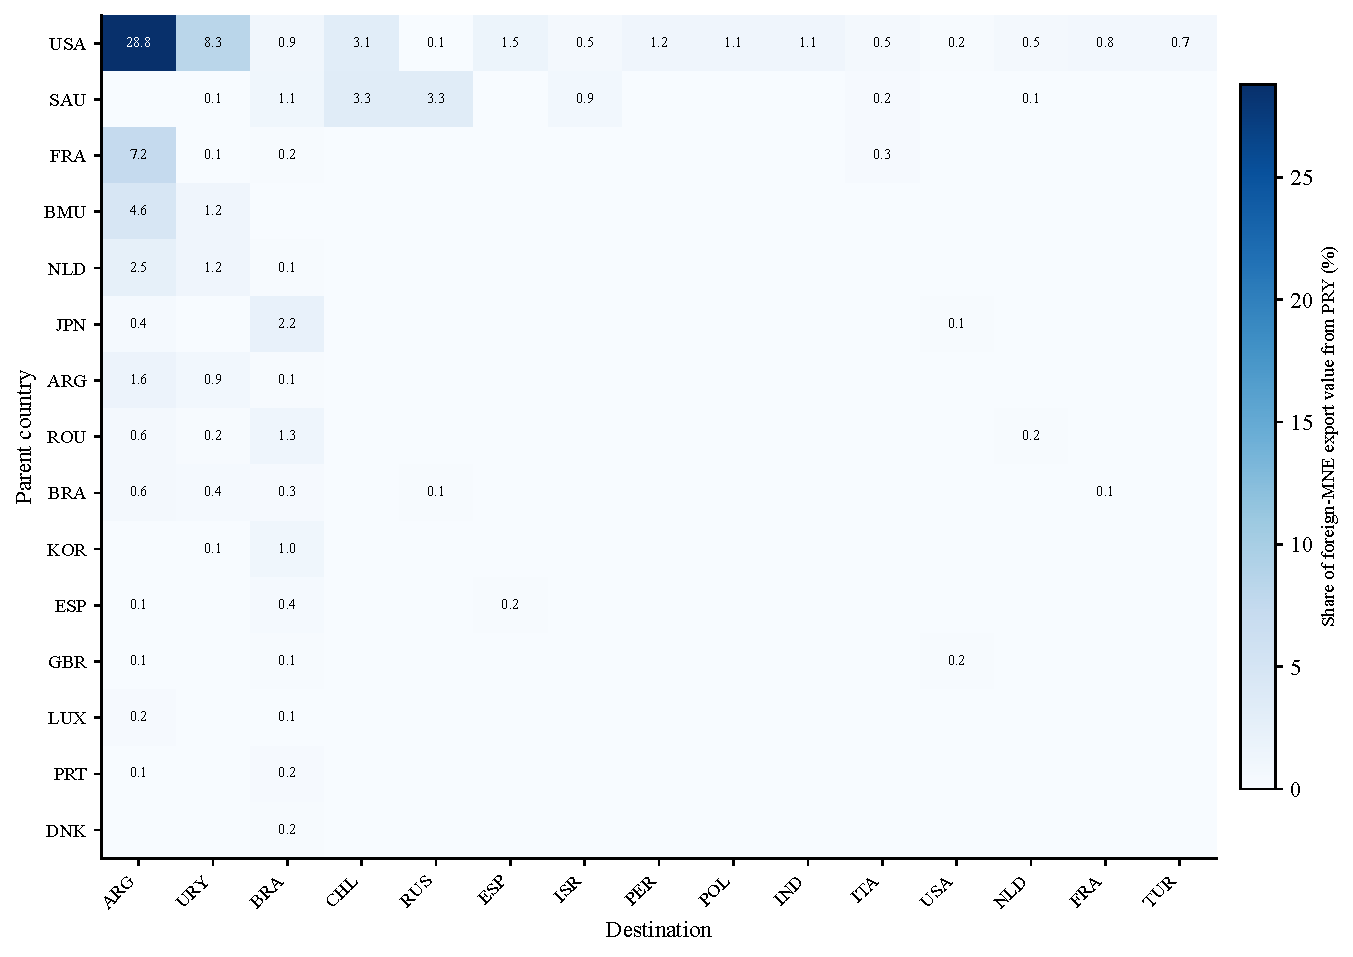
\includegraphics[width=1.0\textwidth,height=0.8\textheight,keepaspectratio]{figures/all/fig_wp1d_heatmap_country_cellpct_PRY.pdf}%
  \caption{Paraguay: Foreign-Multinational Exports by Parent Country and Destination}%
  \label{fig:c_hm_PRY}%
  \par\vspace{2pt}%
  \parbox{0.92\textwidth}{\footnotesize %
  \textit{Notes:} Percent of the foreign-MNE export value of Paraguay in each parent country and destination pair; fifteen largest parent countries and destinations.\\[3pt]%
  \textit{Source:} Authors' calculations based on customs data matched to Orbis and Dun \& Bradstreet.}%
  \end{figure}
% ---- Figure: Paraguay: Share of Foreign-Multinational Exports Shipped to the Parent Country
\begin{figure}[H]\centering%
  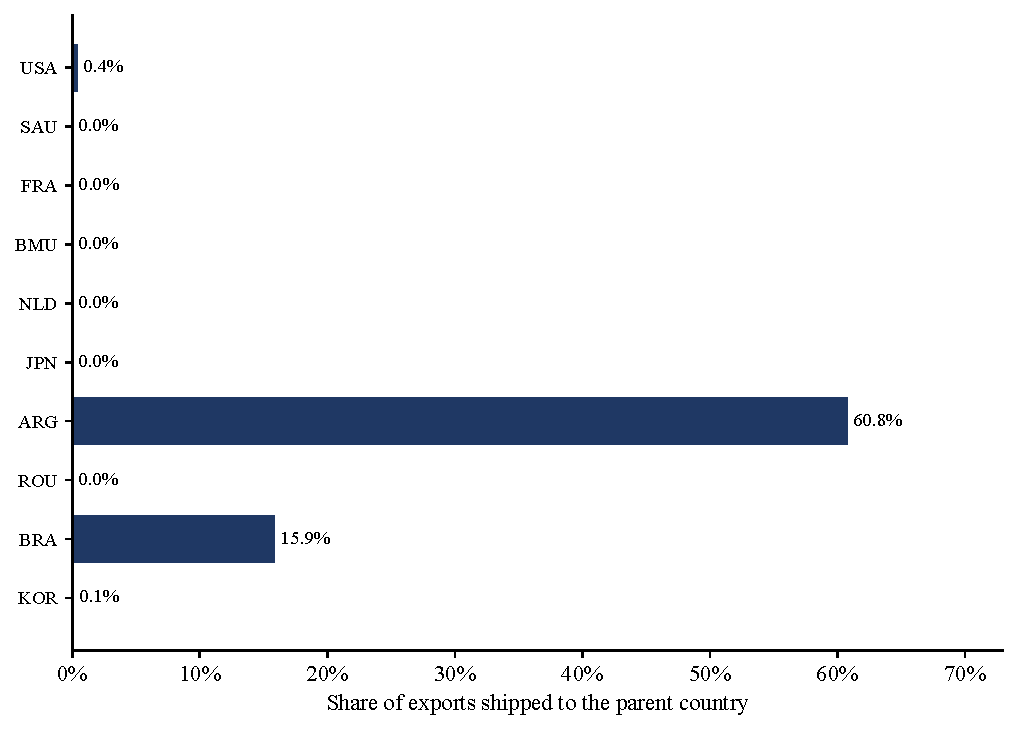
\includegraphics[width=0.85\textwidth,height=0.8\textheight,keepaspectratio]{figures/all/fig_wp1d_home_share_by_parent_PRY.pdf}%
  \caption{Paraguay: Share of Foreign-Multinational Exports Shipped to the Parent Country}%
  \label{fig:c_home_PRY}%
  \par\vspace{2pt}%
  \parbox{0.92\textwidth}{\footnotesize %
  \textit{Notes:} Percent of each parent country's exports from Paraguay shipped to that same country; ten largest parent countries.\\[3pt]%
  \textit{Source:} Authors' calculations based on customs data matched to Orbis and Dun \& Bradstreet.}%
  \end{figure}
% ---- Table: Paraguay, Agriculture: Multinational Exports by Parent Region and Destination Region
\begin{table}[H]\centering\small%
  \caption{Paraguay, Agriculture: Multinational Exports by Parent Region and Destination Region}%
  \label{tab:c_reg_PRY_agro}%
  \adjustbox{max width=\textwidth, max totalheight=0.8\textheight}{\begin{tabular}{lrrrrrrrr}
\toprule
PRY: parent region \ destination & Latin America & North America & Europe & Asia & Africa & Oceania & Rest of World & Total \\
\midrule
Latin America & 96.3 & 0.0 & 3.4 & 0.2 & 0.0 & 0.0 & 0.0 & 0.4 \\
North America & 79.1 & 0.4 & 12.1 & 7.1 & 1.4 & 0.0 & 0.0 & 2.2 \\
Europe & 92.0 & 1.5 & 5.2 & 1.1 & 0.1 & 0.1 & 0.0 & 0.6 \\
Asia & 40.0 & 0.0 & 31.7 & 24.5 & 3.8 & 0.0 & 0.0 & 0.5 \\
Africa & 97.1 & 0.0 & 2.2 & 0.5 & 0.1 & 0.0 & 0.0 & 0.0 \\
Rest of World & 100.0 & 0.0 & 0.0 & 0.0 & 0.0 & 0.0 & 0.0 & 0.0 \\
Domestic MNEs & 83.9 & 0.2 & 10.9 & 0.9 & 4.2 & 0.0 & 0.0 & 0.1 \\
Local firms & 62.9 & 3.1 & 21.7 & 10.8 & 1.4 & 0.0 & 0.0 & 2.1 \\
\bottomrule
\end{tabular}
}%
  \par\vspace{3pt}%
  \begin{minipage}{0.95\textwidth}\footnotesize %
  \textit{Notes:} Percent of each group's agricultural exports from Paraguay, by destination region (rows add to 100). Last column: the group's exports. Values are annual averages in US\$ billion.\\[3pt]%
  \textit{Source:} Authors' calculations based on customs data matched to Orbis and Dun \& Bradstreet.%
  \end{minipage}%
  \end{table}
% ---- Table: Paraguay, Manufacturing: Multinational Exports by Parent Region and Destination Region
\begin{table}[H]\centering\small%
  \caption{Paraguay, Manufacturing: Multinational Exports by Parent Region and Destination Region}%
  \label{tab:c_reg_PRY_manufacturing}%
  \adjustbox{max width=\textwidth, max totalheight=0.8\textheight}{\begin{tabular}{lrrrrrrrr}
\toprule
PRY: parent region \ destination & Latin America & North America & Europe & Asia & Africa & Oceania & Rest of World & Total \\
\midrule
Latin America & 79.1 & 7.5 & 10.2 & 3.2 & 0.0 & 0.0 & 0.0 & 0.0 \\
North America & 94.5 & 5.4 & 0.1 & 0.0 & 0.0 & 0.0 & 0.0 & 0.0 \\
Europe & 82.6 & 2.2 & 9.8 & 5.2 & 0.1 & 0.0 & 0.0 & 0.1 \\
Asia & 84.0 & 4.9 & 8.8 & 2.3 & 0.0 & 0.0 & 0.0 & 0.2 \\
Africa & 30.3 & 67.8 & 0.4 & 1.5 & 0.0 & 0.0 & 0.0 & 0.0 \\
Rest of World & 100.0 & 0.0 & 0.0 & 0.0 & 0.0 & 0.0 & 0.0 & 0.0 \\
Domestic MNEs & 94.0 & 1.6 & 1.7 & 2.7 & 0.0 & 0.0 & 0.0 & 0.0 \\
Local firms & 69.5 & 4.7 & 15.0 & 10.6 & 0.1 & 0.0 & 0.0 & 0.6 \\
\bottomrule
\end{tabular}
}%
  \par\vspace{3pt}%
  \begin{minipage}{0.95\textwidth}\footnotesize %
  \textit{Notes:} Percent of each group's manufacturing exports from Paraguay, by destination region (rows add to 100). Last column: the group's exports. Values are annual averages in US\$ billion.\\[3pt]%
  \textit{Source:} Authors' calculations based on customs data matched to Orbis and Dun \& Bradstreet.%
  \end{minipage}%
  \end{table}
% ---- Table: Paraguay, Mining and Fuels: Multinational Exports by Parent Region and Destination Region
\begin{table}[H]\centering\small%
  \caption{Paraguay, Mining and Fuels: Multinational Exports by Parent Region and Destination Region}%
  \label{tab:c_reg_PRY_mining}%
  \adjustbox{max width=\textwidth, max totalheight=0.8\textheight}{\begin{tabular}{lrrrrrr}
\toprule
PRY: parent region \ destination & Latin America & North America & Europe & Asia & Africa & Total \\
\midrule
Latin America & 99.6 & 0.4 & 0.0 & 0.0 & 0.0 & 0.0 \\
North America & 0.1 & 99.9 & 0.0 & 0.0 & 0.1 & 0.0 \\
Europe & 45.3 & 0.9 & 53.8 & 0.0 & 0.0 & 0.0 \\
Asia & 0.1 & 96.5 & 3.0 & 0.3 & 0.0 & 0.0 \\
Domestic MNEs & 99.3 & 0.5 & 0.2 & 0.0 & 0.0 & 0.0 \\
Local firms & 85.2 & 13.0 & 1.0 & 0.7 & 0.0 & 0.0 \\
\bottomrule
\end{tabular}
}%
  \par\vspace{3pt}%
  \begin{minipage}{0.95\textwidth}\footnotesize %
  \textit{Notes:} Percent of each group's mining and fuels exports from Paraguay, by destination region (rows add to 100). Last column: the group's exports. Values are annual averages in US\$ billion.\\[3pt]%
  \textit{Source:} Authors' calculations based on customs data matched to Orbis and Dun \& Bradstreet.%
  \end{minipage}%
  \end{table}

\subsection{Products}
% ---- Table: Paraguay: Fifteen Largest Export Products
\begin{table}[H]\centering\footnotesize%
  \caption{Paraguay: Fifteen Largest Export Products}%
  \label{tab:c_hs6_PRY}%
  \adjustbox{max width=\textwidth, max totalheight=0.8\textheight}{\begin{tabular}{@{}l p{6.4cm} r r r r l@{}}
\toprule
HS6 & Description & US\$bn/yr & Foreign (\%) & Domestic (\%) & Local (\%) & Leading parent \\
\midrule
120100 & Soya beans, whether/\allowbreak{}not broken & 2.3 & 75 & 1 & 24 & USA (0.63) \\
230400 & Oil-cake and other solid residues, whether/\allowbreak{}not ground/\allowbreak{}in pellets, from extraction of soyabean ... & 1.0 & 88 & 0 & 12 & USA (0.77) \\
020230 & Meat of bovine animals, frozen, boneless & 0.6 & 36 & 0 & 64 & SAU (1.00) \\
150710 & Soya bean oil, crude, whether/\allowbreak{}not degummed, not chemically modified & 0.5 & 89 & 0 & 11 & USA (0.77) \\
100590 & Maize (corn), other than seed & 0.4 & 69 & 1 & 29 & USA (0.71) \\
020130 & Meat of bovine animals, fresh/\allowbreak{}chilled, boneless & 0.4 & 44 & 0 & 56 & SAU (1.00) \\
854430 & Ignition wiring sets and other wiring sets of a kind used in vehicles/\allowbreak{}aircraft/\allowbreak{}ships & 0.1 & 100 & 0 & 0 & JPN (0.71) \\
100190 & Wheat other than durum wheat; meslin & 0.1 & 42 & 2 & 55 & USA (0.41) \\
100630 & Semi-milled/\allowbreak{}wholly milled rice, whether/\allowbreak{}not polished/\allowbreak{}glazed & 0.1 & 27 & 12 & 61 & DNK (0.24) \\
410411 & Tanned/\allowbreak{}crust hides and skins of bovine (incl. buffalo)/\allowbreak{}equine animals, without hair on, in the... & 0.1 & 17 & 0 & 83 & SAU (0.93) \\
170111 & Cane sugar, raw, in solid form, not containing added flavouring/\allowbreak{}colouring matter & 0.1 & 0 & 0 & 100 & DEU (1.00) \\
392330 & Carboys, bottles, flasks and similar articles, of plastics & 0.1 & 0 & 0 & 100 & KOR (0.45) \\
050400 & Guts, bladders and stomachs of animals (other than fish), whole and pieces thereof , fresh/\allowbreak{}chi... & 0.1 & 52 & 0 & 48 & BRA (0.55) \\
100620 & Husked (brown) rice & 0.0 & 33 & 9 & 59 & ECU (0.58) \\
120740 & Sesamum seeds, whether/\allowbreak{}not broken & 0.0 & 14 & 0 & 86 & GBR (0.37) \\
\bottomrule
\end{tabular}
}%
  \par\vspace{3pt}%
  \begin{minipage}{0.95\textwidth}\footnotesize %
  \textit{Notes:} Fifteen largest HS6 products exported by Paraguay. Foreign, domestic and local: percent of the product's export value. Leading parent: largest parent country and its share of the product's foreign-MNE exports. Values are annual averages in US\$ billion.\\[3pt]%
  \textit{Source:} Authors' calculations based on customs data matched to Orbis and Dun \& Bradstreet.%
  \end{minipage}%
  \end{table}
% ---- Table: Paraguay, Agriculture: Fifteen Largest Export Products
\begin{table}[H]\centering\footnotesize%
  \caption{Paraguay, Agriculture: Fifteen Largest Export Products}%
  \label{tab:c_hs6_PRY_agro}%
  \adjustbox{max width=\textwidth, max totalheight=0.8\textheight}{\begin{tabular}{@{}l p{6.4cm} r r r r l@{}}
\toprule
HS6 & Description & US\$bn/yr & Foreign (\%) & Domestic (\%) & Local (\%) & Leading parent \\
\midrule
120100 & Soya beans, whether/\allowbreak{}not broken & 2.3 & 75 & 1 & 24 & USA (0.63) \\
230400 & Oil-cake and other solid residues, whether/\allowbreak{}not ground/\allowbreak{}in pellets, from extraction of soyabean ... & 1.0 & 88 & 0 & 12 & USA (0.77) \\
020230 & Meat of bovine animals, frozen, boneless & 0.6 & 36 & 0 & 64 & SAU (1.00) \\
150710 & Soya bean oil, crude, whether/\allowbreak{}not degummed, not chemically modified & 0.5 & 89 & 0 & 11 & USA (0.77) \\
100590 & Maize (corn), other than seed & 0.4 & 69 & 1 & 29 & USA (0.71) \\
020130 & Meat of bovine animals, fresh/\allowbreak{}chilled, boneless & 0.4 & 44 & 0 & 56 & SAU (1.00) \\
100190 & Wheat other than durum wheat; meslin & 0.1 & 42 & 2 & 55 & USA (0.41) \\
100630 & Semi-milled/\allowbreak{}wholly milled rice, whether/\allowbreak{}not polished/\allowbreak{}glazed & 0.1 & 27 & 12 & 61 & DNK (0.24) \\
170111 & Cane sugar, raw, in solid form, not containing added flavouring/\allowbreak{}colouring matter & 0.1 & 0 & 0 & 100 & DEU (1.00) \\
050400 & Guts, bladders and stomachs of animals (other than fish), whole and pieces thereof , fresh/\allowbreak{}chi... & 0.1 & 52 & 0 & 48 & BRA (0.55) \\
100620 & Husked (brown) rice & 0.0 & 33 & 9 & 59 & ECU (0.58) \\
120740 & Sesamum seeds, whether/\allowbreak{}not broken & 0.0 & 14 & 0 & 86 & GBR (0.37) \\
120799 & Oil seeds and oleaginous fruits (excl. of 1206.00 and 1207.20-1207.91), whether/\allowbreak{}not broken & 0.0 & 43 & 0 & 57 & GBR (0.74) \\
020629 & Edible offal of bovine animals (excl. tongues and livers), frozen & 0.0 & 46 & 0 & 54 & SAU (1.00) \\
240220 & Cigarettes containing tobacco & 0.0 & 13 & 0 & 87 & URY (1.00) \\
\bottomrule
\end{tabular}
}%
  \par\vspace{3pt}%
  \begin{minipage}{0.95\textwidth}\footnotesize %
  \textit{Notes:} Fifteen largest agricultural HS6 products exported by Paraguay. Foreign, domestic and local: percent of the product's export value. Leading parent: largest parent country and its share of the product's foreign-MNE exports. Values are annual averages in US\$ billion.\\[3pt]%
  \textit{Source:} Authors' calculations based on customs data matched to Orbis and Dun \& Bradstreet.%
  \end{minipage}%
  \end{table}
% ---- Table: Paraguay, Manufacturing: Fifteen Largest Export Products
\begin{table}[H]\centering\footnotesize%
  \caption{Paraguay, Manufacturing: Fifteen Largest Export Products}%
  \label{tab:c_hs6_PRY_manufacturing}%
  \adjustbox{max width=\textwidth, max totalheight=0.8\textheight}{\begin{tabular}{@{}l p{6.4cm} r r r r l@{}}
\toprule
HS6 & Description & US\$bn/yr & Foreign (\%) & Domestic (\%) & Local (\%) & Leading parent \\
\midrule
854430 & Ignition wiring sets and other wiring sets of a kind used in vehicles/\allowbreak{}aircraft/\allowbreak{}ships & 0.15 & 100 & 0 & 0 & JPN (0.71) \\
410411 & Tanned/\allowbreak{}crust hides and skins of bovine (incl. buffalo)/\allowbreak{}equine animals, without hair on, in the... & 0.08 & 17 & 0 & 83 & SAU (0.93) \\
392330 & Carboys, bottles, flasks and similar articles, of plastics & 0.06 & 0 & 0 & 100 & KOR (0.45) \\
630140 & Blankets (excl. electric) and travelling rugs, of synthetic fibres & 0.04 & 13 & 7 & 80 & FRA (0.84) \\
440290 & Wood charcoal (including shell/\allowbreak{}nut charcoal, excl. of 440210), whether/\allowbreak{}not agglomerated. & 0.03 & 46 & 1 & 52 & ESP (0.86) \\
300490 & Medicaments (excluding goods of heading 30.02/\allowbreak{}30.05/\allowbreak{}30.06/\allowbreak{}3004.10-3004.50) consisting of mixed... & 0.03 & 1 & 0 & 99 & DEU (0.94) \\
410441 & Tanned/\allowbreak{}crust hides and skins of bovine (incl. buffalo)/\allowbreak{}equine animals, without hair on, in the... & 0.02 & 1 & 0 & 99 & TWN (1.00) \\
740400 & Copper waste and scrap & 0.02 & 4 & 0 & 96 & PER (0.57) \\
760200 & Aluminium waste and scrap & 0.02 & 1 & 0 & 99 & BRA (0.39) \\
380891 & Insecticides, put up in forms/\allowbreak{}packings for retail sale/\allowbreak{}as preparations/\allowbreak{}articles  & 0.02 & 9 & 0 & 90 & CHN (0.57) \\
890190 & Vessels for the transportof goods and for the transportof both persons and goods (excl. of 890... & 0.02 & 97 & 0 & 3 & KOR (0.49) \\
720449 & Ferrous waste and scrap (excl. of 7204.10-7204.41) & 0.01 & 11 & 2 & 87 & BRA (0.82) \\
701090 & Carboys, bottles, flasks, jars, pots, phials and other containters, of glass, of a kind used f... & 0.01 & 100 & 0 & 0 & LUX (0.98) \\
640610 & Uppers and parts thereof (excl. stiffeners), whether/\allowbreak{}not attached to soles other than outer so... & 0.01 & 94 & 0 & 6 & -- \\
560122 & Wadding; other articles of wadding, of man-made fibres & 0.01 & 50 & 50 & 0 & GBR (1.00) \\
\bottomrule
\end{tabular}
}%
  \par\vspace{3pt}%
  \begin{minipage}{0.95\textwidth}\footnotesize %
  \textit{Notes:} Fifteen largest manufacturing HS6 products exported by Paraguay. Foreign, domestic and local: percent of the product's export value. Leading parent: largest parent country and its share of the product's foreign-MNE exports. Values are annual averages in US\$ billion.\\[3pt]%
  \textit{Source:} Authors' calculations based on customs data matched to Orbis and Dun \& Bradstreet.%
  \end{minipage}%
  \end{table}
% ---- Table: Paraguay, Mining and Fuels: Fifteen Largest Export Products
\begin{table}[H]\centering\footnotesize%
  \caption{Paraguay, Mining and Fuels: Fifteen Largest Export Products}%
  \label{tab:c_hs6_PRY_mining}%
  \adjustbox{max width=\textwidth, max totalheight=0.8\textheight}{\begin{tabular}{@{}l p{6.4cm} r r r r l@{}}
\toprule
HS6 & Description & US\$bn/yr & Foreign (\%) & Domestic (\%) & Local (\%) & Leading parent \\
\midrule
271019 & Petroleum oils and oils obtained from bituminous minerals (other than crude) and preparations ... & 0.04 & 18 & 0 & 82 & DNK (0.49) \\
710813 & Gold (incl. gold plated with platinum), non-monetary, in semi-manufactured forms & 0.02 & 74 & 0 & 26 & FRA (0.69) \\
271011 & Light petroleum oils and preparations & 0.01 & 70 & 0 & 30 & BRA (0.38) \\
251710 & Pebbles/\allowbreak{}gravel/\allowbreak{}broken/\allowbreak{}crushed stone, of a kind commonly used for concrete aggregates/\allowbreak{}road meta... & 0.00 & 82 & 10 & 8 & HUN (1.00) \\
271119 & Petroleum gases other than natural gas/\allowbreak{}propane/\allowbreak{}butanes/\allowbreak{}ethylene, propylene, butylene and butad... & 0.00 & 26 & 0 & 74 & -- \\
271113 & Butanes, liquefied & 0.00 & 18 & 0 & 82 & -- \\
710812 & Gold (incl. gold plated with platinum), in unwrought forms (excl. powder) & 0.00 & 62 & 0 & 38 & CAN (1.00) \\
711590 & Articles of precious metal/\allowbreak{}metal clad with precious metal, n.e.s. in Ch.71 & 0.00 & 100 & 0 & 0 & FRA (0.96) \\
251749 & Granules, chippings and powder, of stones of 25.15/\allowbreak{}25.16 (excl. marble), whether/\allowbreak{}not heat-trea... & 0.00 & 0 & 0 & 100 & -- \\
711019 & Platinum, in semi-manufactured forms & 0.00 & 99 & 0 & 1 & FRA (1.00) \\
711890 & Other coin (excl. of 7118.10) & 0.00 & 13 & 0 & 87 & URY (1.00) \\
271311 & Petroleum coke, not calcined & 0.00 & 100 & 0 & 0 & FRA (1.00) \\
711790 & Imitation jewellery other than of base metal & 0.00 & 0 & 0 & 100 & URY (1.00) \\
262190 & Slag and ash, incl. seaweed ash (kelp), other than ash and residues from the incineration of m... & 0.00 & 1 & 75 & 24 & CHE (1.00) \\
271500 & Bituminous mixtures based on natural asphalt/\allowbreak{}natural bitumen/\allowbreak{}petroleum bitumen/\allowbreak{}mineral tar/\allowbreak{}min... & 0.00 & 82 & 0 & 18 & CHE (1.00) \\
\bottomrule
\end{tabular}
}%
  \par\vspace{3pt}%
  \begin{minipage}{0.95\textwidth}\footnotesize %
  \textit{Notes:} Fifteen largest mining and fuels HS6 products exported by Paraguay. Foreign, domestic and local: percent of the product's export value. Leading parent: largest parent country and its share of the product's foreign-MNE exports. Values are annual averages in US\$ billion.\\[3pt]%
  \textit{Source:} Authors' calculations based on customs data matched to Orbis and Dun \& Bradstreet.%
  \end{minipage}%
  \end{table}

\section{El Salvador}\label{sec:c_SLV}

\subsection{Parents and Destinations}
% ---- Table: El Salvador: Multinational Exports by Parent Region and Destination Region
\begin{table}[H]\centering\small%
  \caption{El Salvador: Multinational Exports by Parent Region and Destination Region}%
  \label{tab:c_reg_SLV}%
  \adjustbox{max width=\textwidth, max totalheight=0.8\textheight}{\begin{tabular}{lrrrrrrrr}
\toprule
SLV: parent region \ destination & Latin America & North America & Europe & Asia & Africa & Oceania & Rest of World & Total \\
\midrule
Latin America & 84.2 & 11.7 & 3.1 & 0.8 & 0.0 & 0.2 & 0.0 & 0.4 \\
North America & 34.4 & 64.5 & 0.7 & 0.3 & 0.0 & 0.0 & 0.0 & 1.5 \\
Europe & 60.3 & 12.9 & 25.2 & 0.7 & 0.3 & 0.6 & 0.0 & 0.3 \\
Asia & 34.0 & 63.4 & 1.6 & 1.0 & 0.0 & 0.1 & 0.0 & 0.1 \\
Africa & 17.9 & 82.0 & 0.1 & 0.0 & 0.0 & 0.0 & 0.0 & 0.0 \\
Oceania & 75.7 & 16.6 & 0.1 & 7.5 & 0.0 & 0.0 & 0.0 & 0.0 \\
Rest of World & 5.7 & 92.9 & 0.0 & 1.4 & 0.0 & 0.0 & 0.0 & 0.0 \\
Domestic MNEs & 99.6 & 0.3 & 0.0 & 0.0 & 0.0 & 0.0 & 0.0 & 0.0 \\
Local firms & 44.9 & 46.3 & 4.6 & 3.7 & 0.1 & 0.3 & 0.1 & 2.6 \\
\bottomrule
\end{tabular}
}%
  \par\vspace{3pt}%
  \begin{minipage}{0.95\textwidth}\footnotesize %
  \textit{Notes:} Percent of each group's exports from El Salvador, by destination region (rows add to 100). Last column: the group's exports. Values are annual averages in US\$ billion.\\[3pt]%
  \textit{Source:} Authors' calculations based on customs data matched to Orbis and Dun \& Bradstreet.%
  \end{minipage}%
  \end{table}
% ---- Figure: El Salvador: Foreign-Multinational Exports by Parent Country and Destination
\begin{figure}[H]\centering%
  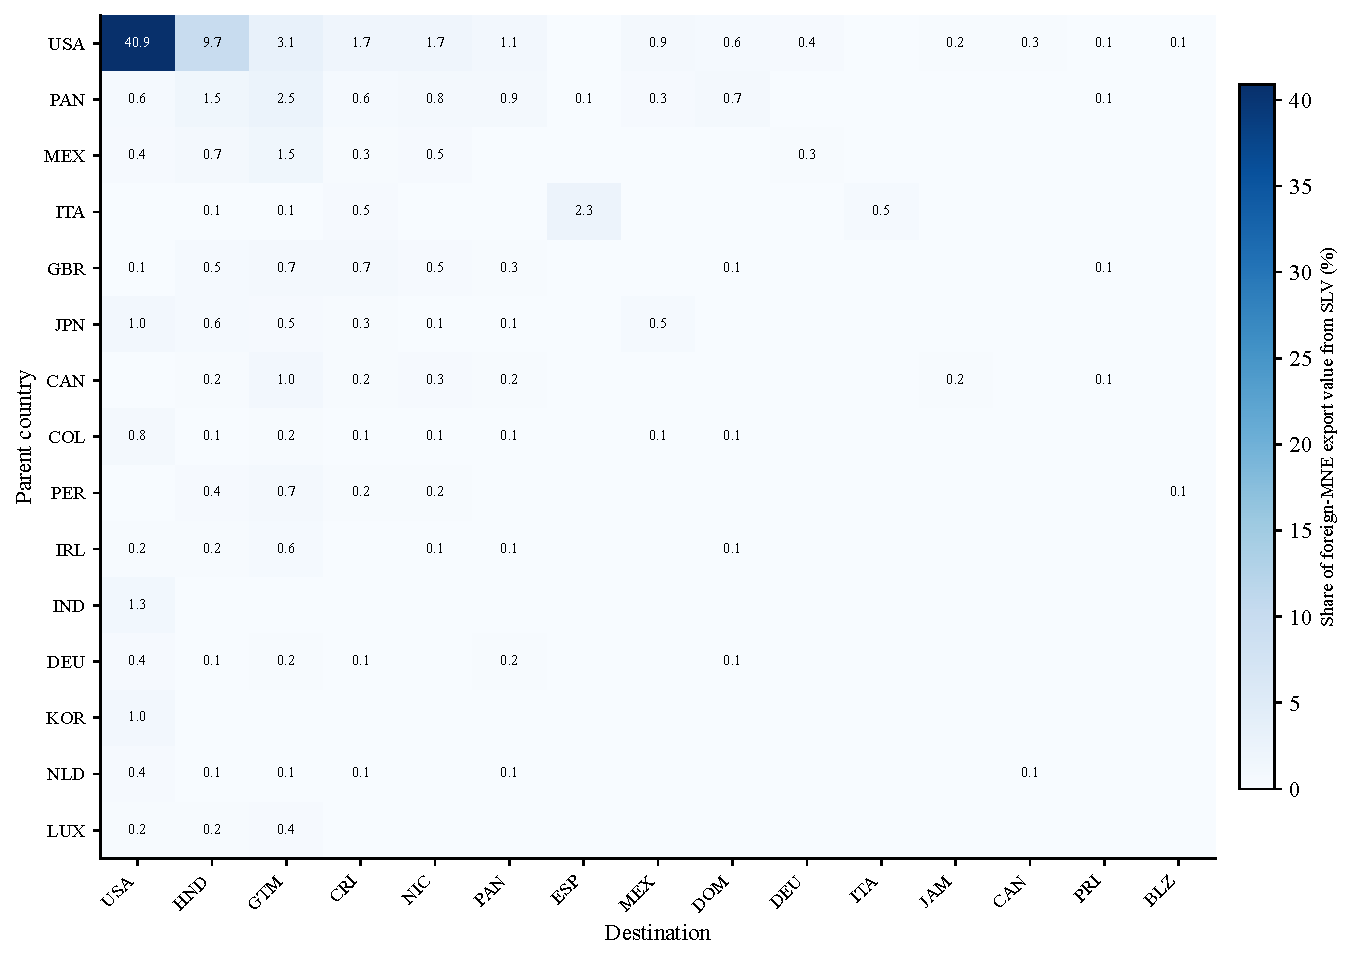
\includegraphics[width=1.0\textwidth,height=0.8\textheight,keepaspectratio]{figures/all/fig_wp1d_heatmap_country_cellpct_SLV.pdf}%
  \caption{El Salvador: Foreign-Multinational Exports by Parent Country and Destination}%
  \label{fig:c_hm_SLV}%
  \par\vspace{2pt}%
  \parbox{0.92\textwidth}{\footnotesize %
  \textit{Notes:} Percent of the foreign-MNE export value of El Salvador in each parent country and destination pair; fifteen largest parent countries and destinations.\\[3pt]%
  \textit{Source:} Authors' calculations based on customs data matched to Orbis and Dun \& Bradstreet.}%
  \end{figure}
% ---- Figure: El Salvador: Share of Foreign-Multinational Exports Shipped to the Parent Country
\begin{figure}[H]\centering%
  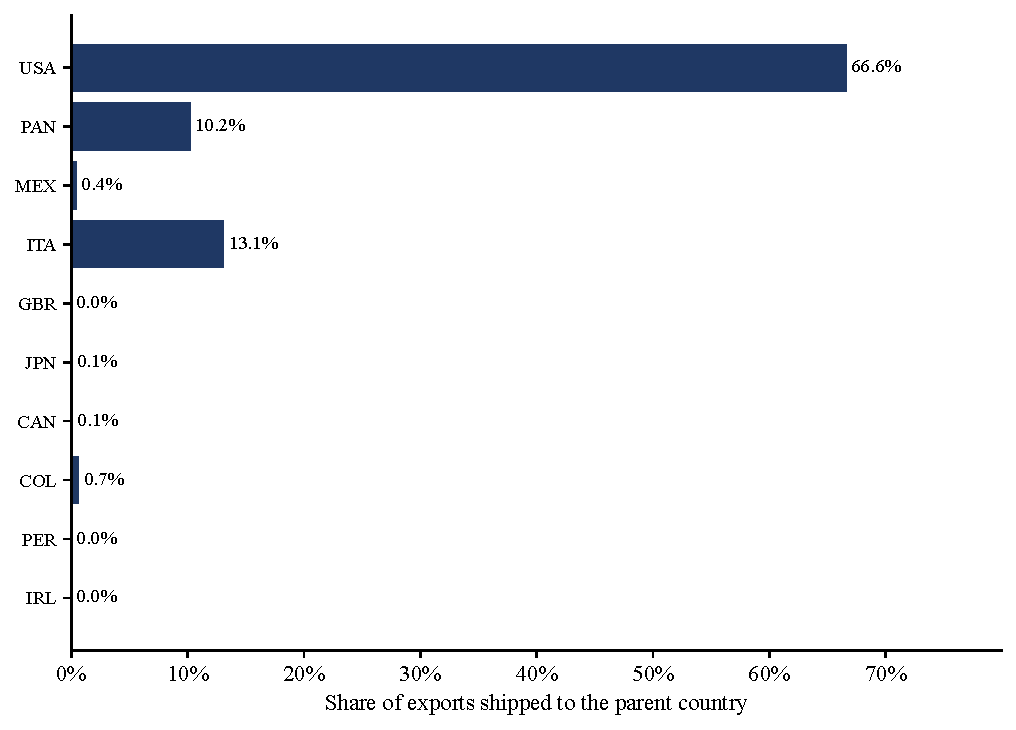
\includegraphics[width=0.85\textwidth,height=0.8\textheight,keepaspectratio]{figures/all/fig_wp1d_home_share_by_parent_SLV.pdf}%
  \caption{El Salvador: Share of Foreign-Multinational Exports Shipped to the Parent Country}%
  \label{fig:c_home_SLV}%
  \par\vspace{2pt}%
  \parbox{0.92\textwidth}{\footnotesize %
  \textit{Notes:} Percent of each parent country's exports from El Salvador shipped to that same country; ten largest parent countries.\\[3pt]%
  \textit{Source:} Authors' calculations based on customs data matched to Orbis and Dun \& Bradstreet.}%
  \end{figure}
% ---- Table: El Salvador, Agriculture: Multinational Exports by Parent Region and Destination Region
\begin{table}[H]\centering\small%
  \caption{El Salvador, Agriculture: Multinational Exports by Parent Region and Destination Region}%
  \label{tab:c_reg_SLV_agro}%
  \adjustbox{max width=\textwidth, max totalheight=0.8\textheight}{\begin{tabular}{lrrrrrrrr}
\toprule
SLV: parent region \ destination & Latin America & North America & Europe & Asia & Africa & Oceania & Rest of World & Total \\
\midrule
Latin America & 81.0 & 11.7 & 5.7 & 1.4 & 0.1 & 0.0 & 0.0 & 0.2 \\
North America & 93.7 & 2.2 & 1.2 & 2.9 & 0.0 & 0.0 & 0.0 & 0.0 \\
Europe & 36.5 & 11.2 & 50.0 & 0.7 & 0.5 & 1.2 & 0.0 & 0.1 \\
Asia & 78.3 & 0.0 & 0.0 & 21.7 & 0.0 & 0.0 & 0.0 & 0.0 \\
Africa & 56.9 & 43.1 & 0.0 & 0.0 & 0.0 & 0.0 & 0.0 & 0.0 \\
Domestic MNEs & 79.6 & 15.2 & 4.1 & 1.0 & 0.0 & 0.0 & 0.0 & 0.0 \\
Local firms & 41.9 & 34.7 & 13.4 & 8.8 & 0.2 & 0.8 & 0.2 & 0.8 \\
\bottomrule
\end{tabular}
}%
  \par\vspace{3pt}%
  \begin{minipage}{0.95\textwidth}\footnotesize %
  \textit{Notes:} Percent of each group's agricultural exports from El Salvador, by destination region (rows add to 100). Last column: the group's exports. Values are annual averages in US\$ billion.\\[3pt]%
  \textit{Source:} Authors' calculations based on customs data matched to Orbis and Dun \& Bradstreet.%
  \end{minipage}%
  \end{table}
% ---- Table: El Salvador, Manufacturing: Multinational Exports by Parent Region and Destination Region
\begin{table}[H]\centering\small%
  \caption{El Salvador, Manufacturing: Multinational Exports by Parent Region and Destination Region}%
  \label{tab:c_reg_SLV_manufacturing}%
  \adjustbox{max width=\textwidth, max totalheight=0.8\textheight}{\begin{tabular}{lrrrrrrrr}
\toprule
SLV: parent region \ destination & Latin America & North America & Europe & Asia & Africa & Oceania & Rest of World & Total \\
\midrule
Latin America & 86.2 & 12.3 & 0.7 & 0.3 & 0.0 & 0.4 & 0.0 & 0.2 \\
North America & 31.4 & 67.5 & 0.8 & 0.3 & 0.0 & 0.0 & 0.0 & 1.4 \\
Europe & 84.8 & 13.3 & 1.1 & 0.8 & 0.1 & 0.0 & 0.0 & 0.1 \\
Asia & 34.0 & 63.4 & 1.6 & 1.0 & 0.0 & 0.1 & 0.0 & 0.1 \\
Africa & 16.5 & 83.5 & 0.0 & 0.0 & 0.0 & 0.0 & 0.0 & 0.0 \\
Oceania & 75.7 & 16.6 & 0.1 & 7.5 & 0.0 & 0.0 & 0.0 & 0.0 \\
Rest of World & 4.7 & 93.9 & 0.0 & 1.4 & 0.0 & 0.0 & 0.0 & 0.0 \\
Domestic MNEs & 99.6 & 0.3 & 0.0 & 0.0 & 0.0 & 0.0 & 0.0 & 0.0 \\
Local firms & 46.4 & 51.1 & 0.9 & 1.5 & 0.1 & 0.0 & 0.0 & 1.8 \\
\bottomrule
\end{tabular}
}%
  \par\vspace{3pt}%
  \begin{minipage}{0.95\textwidth}\footnotesize %
  \textit{Notes:} Percent of each group's manufacturing exports from El Salvador, by destination region (rows add to 100). Last column: the group's exports. Values are annual averages in US\$ billion.\\[3pt]%
  \textit{Source:} Authors' calculations based on customs data matched to Orbis and Dun \& Bradstreet.%
  \end{minipage}%
  \end{table}
% ---- Table: El Salvador, Mining and Fuels: Multinational Exports by Parent Region and Destination Region
\begin{table}[H]\centering\small%
  \caption{El Salvador, Mining and Fuels: Multinational Exports by Parent Region and Destination Region}%
  \label{tab:c_reg_SLV_mining}%
  \adjustbox{max width=\textwidth, max totalheight=0.8\textheight}{\begin{tabular}{lrrrrrrrr}
\toprule
SLV: parent region \ destination & Latin America & North America & Europe & Asia & Africa & Oceania & Rest of World & Total \\
\midrule
Latin America & 87.6 & 7.3 & 5.0 & 0.1 & 0.0 & 0.0 & 0.0 & 0.0 \\
North America & 97.9 & 2.0 & 0.1 & 0.0 & 0.0 & 0.0 & 0.0 & 0.1 \\
Europe & 5.3 & 94.5 & 0.2 & 0.0 & 0.0 & 0.0 & 0.0 & 0.0 \\
Asia & 84.4 & 15.6 & 0.0 & 0.0 & 0.0 & 0.0 & 0.0 & 0.0 \\
Africa & 0.0 & 100.0 & 0.0 & 0.0 & 0.0 & 0.0 & 0.0 & 0.0 \\
Rest of World & 100.0 & 0.0 & 0.0 & 0.0 & 0.0 & 0.0 & 0.0 & 0.0 \\
Domestic MNEs & 99.3 & 0.7 & 0.0 & 0.0 & 0.0 & 0.0 & 0.0 & 0.0 \\
Local firms & 41.3 & 58.1 & 0.1 & 0.5 & 0.0 & 0.0 & 0.0 & 0.1 \\
\bottomrule
\end{tabular}
}%
  \par\vspace{3pt}%
  \begin{minipage}{0.95\textwidth}\footnotesize %
  \textit{Notes:} Percent of each group's mining and fuels exports from El Salvador, by destination region (rows add to 100). Last column: the group's exports. Values are annual averages in US\$ billion.\\[3pt]%
  \textit{Source:} Authors' calculations based on customs data matched to Orbis and Dun \& Bradstreet.%
  \end{minipage}%
  \end{table}
% ---- Table: El Salvador, Other Goods: Multinational Exports by Parent Region and Destination Region
\begin{table}[H]\centering\small%
  \caption{El Salvador, Other Goods: Multinational Exports by Parent Region and Destination Region}%
  \label{tab:c_reg_SLV_rest}%
  \adjustbox{max width=\textwidth, max totalheight=0.8\textheight}{\begin{tabular}{lrrrrrrrr}
\toprule
SLV: parent region \ destination & Latin America & North America & Europe & Asia & Africa & Oceania & Rest of World & Total \\
\midrule
Latin America & 88.9 & 4.6 & 4.2 & 2.3 & 0.0 & 0.0 & 0.0 & 0.0 \\
North America & 100.0 & 0.0 & 0.0 & 0.0 & 0.0 & 0.0 & 0.0 & 0.0 \\
Europe & 43.0 & 23.8 & 29.8 & 3.5 & 0.0 & 0.0 & 0.0 & 0.0 \\
Asia & 0.0 & 100.0 & 0.0 & 0.0 & 0.0 & 0.0 & 0.0 & 0.0 \\
Africa & 62.0 & 18.3 & 19.7 & 0.0 & 0.0 & 0.0 & 0.0 & 0.0 \\
Local firms & 51.9 & 31.7 & 11.1 & 3.5 & 1.2 & 0.5 & 0.0 & 0.0 \\
\bottomrule
\end{tabular}
}%
  \par\vspace{3pt}%
  \begin{minipage}{0.95\textwidth}\footnotesize %
  \textit{Notes:} Percent of each group's exports from El Salvador, by destination region (rows add to 100). Last column: the group's exports. Values are annual averages in US\$ billion.\\[3pt]%
  \textit{Source:} Authors' calculations based on customs data matched to Orbis and Dun \& Bradstreet.%
  \end{minipage}%
  \end{table}

\subsection{Products}
% ---- Table: El Salvador: Fifteen Largest Export Products
\begin{table}[H]\centering\footnotesize%
  \caption{El Salvador: Fifteen Largest Export Products}%
  \label{tab:c_hs6_SLV}%
  \adjustbox{max width=\textwidth, max totalheight=0.8\textheight}{\begin{tabular}{@{}l p{6.4cm} r r r r l@{}}
\toprule
HS6 & Description & US\$bn/yr & Foreign (\%) & Domestic (\%) & Local (\%) & Leading parent \\
\midrule
610910 & T-shirts, singlets and other vests, knitted/\allowbreak{}crocheted, of cotton & 0.67 & 71 & 0 & 29 & USA (0.98) \\
090111 & Coffee, not roasted, not decaffeinated & 0.21 & 20 & 0 & 80 & MEX (0.89) \\
611020 & Jerseys, pullovers, cardigans, waist-coats and similar articles, knitted/\allowbreak{}crocheted, of cotton & 0.13 & 47 & 0 & 53 & USA (0.97) \\
853221 & Fixed electrical capacitors, other than those of 8532.10, tantalum & 0.12 & 0 & 0 & 100 & -- \\
610711 & Men's/\allowbreak{}boys' underpants and briefs, knitted/\allowbreak{}crocheted, of cotton & 0.11 & 90 & 0 & 10 & USA (1.00) \\
481810 & Toilet paper, in rolls of a width not >36cm/\allowbreak{}cut to size/\allowbreak{}shape & 0.11 & 70 & 0 & 30 & USA (1.00) \\
611030 & Jerseys, pullovers, cardigans, waist-coats and similar articles, knitted/\allowbreak{}crocheted, of man-mad... & 0.11 & 43 & 0 & 57 & USA (0.39) \\
611595 & Other n.e.s. in 61.15, knitted/\allowbreak{}crocheted, of cotton. & 0.10 & 100 & 0 & 0 & USA (1.00) \\
170114 & Cane sugar, raw, in solid form, not containing added flavouring/\allowbreak{}colouring matter [later HS rev... & 0.09 & 0 & 0 & 100 & BGR (0.66) \\
160414 & Tunas, skipjack and bonito (Sarda spp.), prepared/\allowbreak{}preserved, whole/\allowbreak{}in pieces (excl. minced) & 0.08 & 92 & 0 & 8 & ITA (1.00) \\
610990 & T-shirts, singlets and other vests, knitted/\allowbreak{}crocheted, other than of cotton & 0.08 & 42 & 0 & 58 & USA (0.68) \\
271019 & Petroleum oils and oils obtained from bituminous minerals (other than crude) and preparations ... & 0.08 & 97 & 0 & 3 & USA (0.74) \\
392330 & Carboys, bottles, flasks and similar articles, of plastics & 0.08 & 75 & 0 & 25 & CAN (0.97) \\
300490 & Medicaments (excluding goods of heading 30.02/\allowbreak{}30.05/\allowbreak{}30.06/\allowbreak{}3004.10-3004.50) consisting of mixed... & 0.08 & 29 & 0 & 71 & COL (0.56) \\
190590 & Bread, pastry, cakes, biscuits and other bakers' wares, whether/\allowbreak{}not containing cocoa; communio... & 0.06 & 11 & 0 & 89 & MEX (0.99) \\
\bottomrule
\end{tabular}
}%
  \par\vspace{3pt}%
  \begin{minipage}{0.95\textwidth}\footnotesize %
  \textit{Notes:} Fifteen largest HS6 products exported by El Salvador. Foreign, domestic and local: percent of the product's export value. Leading parent: largest parent country and its share of the product's foreign-MNE exports. Values are annual averages in US\$ billion.\\[3pt]%
  \textit{Source:} Authors' calculations based on customs data matched to Orbis and Dun \& Bradstreet.%
  \end{minipage}%
  \end{table}
% ---- Table: El Salvador, Agriculture: Fifteen Largest Export Products
\begin{table}[H]\centering\footnotesize%
  \caption{El Salvador, Agriculture: Fifteen Largest Export Products}%
  \label{tab:c_hs6_SLV_agro}%
  \adjustbox{max width=\textwidth, max totalheight=0.8\textheight}{\begin{tabular}{@{}l p{6.4cm} r r r r l@{}}
\toprule
HS6 & Description & US\$bn/yr & Foreign (\%) & Domestic (\%) & Local (\%) & Leading parent \\
\midrule
090111 & Coffee, not roasted, not decaffeinated & 0.21 & 20 & 0 & 80 & MEX (0.89) \\
170114 & Cane sugar, raw, in solid form, not containing added flavouring/\allowbreak{}colouring matter [later HS rev... & 0.09 & 0 & 0 & 100 & BGR (0.66) \\
160414 & Tunas, skipjack and bonito (Sarda spp.), prepared/\allowbreak{}preserved, whole/\allowbreak{}in pieces (excl. minced) & 0.08 & 92 & 0 & 8 & ITA (1.00) \\
190590 & Bread, pastry, cakes, biscuits and other bakers' wares, whether/\allowbreak{}not containing cocoa; communio... & 0.06 & 11 & 0 & 89 & MEX (0.99) \\
220290 & Non-alcoholic beverages other than waters of 2202.10 (not incl. fruit/\allowbreak{}vegetable juices of 20.0... & 0.06 & 96 & 0 & 4 & PAN (1.00) \\
220710 & Undenatured ethyl alcohol of an alcoholic strength by volume of 80\% vol. & 0.06 & 0 & 0 & 100 & FRA (1.00) \\
170111 & Cane sugar, raw, in solid form, not containing added flavouring/\allowbreak{}colouring matter & 0.04 & 0 & 0 & 100 & PAN (0.81) \\
110220 & Maize (corn) flour & 0.03 & 18 & 0 & 82 & MEX (0.94) \\
190410 & Prepared foods obt. by the swelling/\allowbreak{}roasting of cereals/\allowbreak{}cereal products & 0.03 & 0 & 0 & 100 & USA (0.83) \\
170490 & Sugar confectionery other than chewing gum (incl. white chocolate), not containing cocoa & 0.03 & 0 & 0 & 100 & GTM (0.36) \\
170310 & Cane molasses & 0.02 & 0 & 0 & 100 & -- \\
220210 & Waters, incl. mineral waters and aerated waters, containing added sugar/\allowbreak{}other sweetening matte... & 0.02 & 60 & 0 & 40 & LUX (0.83) \\
210690 & Food preparations, n.e.s. & 0.02 & 5 & 0 & 95 & DEU (0.46) \\
190531 & Sweet biscuits & 0.02 & 1 & 0 & 99 & ITA (0.31) \\
170199 & Cane/\allowbreak{}beet sugar and chemically pure sucrose, in solid form, not containing added flavouring/\allowbreak{}co... & 0.02 & 0 & 0 & 100 & VEN (0.99) \\
\bottomrule
\end{tabular}
}%
  \par\vspace{3pt}%
  \begin{minipage}{0.95\textwidth}\footnotesize %
  \textit{Notes:} Fifteen largest agricultural HS6 products exported by El Salvador. Foreign, domestic and local: percent of the product's export value. Leading parent: largest parent country and its share of the product's foreign-MNE exports. Values are annual averages in US\$ billion.\\[3pt]%
  \textit{Source:} Authors' calculations based on customs data matched to Orbis and Dun \& Bradstreet.%
  \end{minipage}%
  \end{table}
% ---- Table: El Salvador, Manufacturing: Fifteen Largest Export Products
\begin{table}[H]\centering\footnotesize%
  \caption{El Salvador, Manufacturing: Fifteen Largest Export Products}%
  \label{tab:c_hs6_SLV_manufacturing}%
  \adjustbox{max width=\textwidth, max totalheight=0.8\textheight}{\begin{tabular}{@{}l p{6.4cm} r r r r l@{}}
\toprule
HS6 & Description & US\$bn/yr & Foreign (\%) & Domestic (\%) & Local (\%) & Leading parent \\
\midrule
610910 & T-shirts, singlets and other vests, knitted/\allowbreak{}crocheted, of cotton & 0.67 & 71 & 0 & 29 & USA (0.98) \\
611020 & Jerseys, pullovers, cardigans, waist-coats and similar articles, knitted/\allowbreak{}crocheted, of cotton & 0.13 & 47 & 0 & 53 & USA (0.97) \\
853221 & Fixed electrical capacitors, other than those of 8532.10, tantalum & 0.12 & 0 & 0 & 100 & -- \\
610711 & Men's/\allowbreak{}boys' underpants and briefs, knitted/\allowbreak{}crocheted, of cotton & 0.11 & 90 & 0 & 10 & USA (1.00) \\
481810 & Toilet paper, in rolls of a width not >36cm/\allowbreak{}cut to size/\allowbreak{}shape & 0.11 & 70 & 0 & 30 & USA (1.00) \\
611030 & Jerseys, pullovers, cardigans, waist-coats and similar articles, knitted/\allowbreak{}crocheted, of man-mad... & 0.11 & 43 & 0 & 57 & USA (0.39) \\
611595 & Other n.e.s. in 61.15, knitted/\allowbreak{}crocheted, of cotton. & 0.10 & 100 & 0 & 0 & USA (1.00) \\
610990 & T-shirts, singlets and other vests, knitted/\allowbreak{}crocheted, other than of cotton & 0.08 & 42 & 0 & 58 & USA (0.68) \\
392330 & Carboys, bottles, flasks and similar articles, of plastics & 0.08 & 75 & 0 & 25 & CAN (0.97) \\
300490 & Medicaments (excluding goods of heading 30.02/\allowbreak{}30.05/\allowbreak{}30.06/\allowbreak{}3004.10-3004.50) consisting of mixed... & 0.08 & 29 & 0 & 71 & COL (0.56) \\
621210 & BrassiFres and parts thereof , whether/\allowbreak{}not knitted/\allowbreak{}crocheted & 0.06 & 99 & 0 & 1 & USA (1.00) \\
392321 & Sacks and bags (incl. cones), of polymers of ethylene & 0.05 & 3 & 0 & 97 & USA (0.68) \\
610462 & Women's/\allowbreak{}girls' trousers, bib and brace overalls, breeches and shorts (excl. swimwear), knitted... & 0.04 & 57 & 0 & 43 & USA (0.99) \\
611521 & Panty hose, tights, stockings, socks and other hosiery, and footwear without applied soles, of... & 0.04 & 100 & 0 & 0 & USA (1.00) \\
620520 & Men's/\allowbreak{}boys' shirts (excl. knitted/\allowbreak{}crocheted), of cotton & 0.04 & 30 & 0 & 70 & DEU (0.95) \\
\bottomrule
\end{tabular}
}%
  \par\vspace{3pt}%
  \begin{minipage}{0.95\textwidth}\footnotesize %
  \textit{Notes:} Fifteen largest manufacturing HS6 products exported by El Salvador. Foreign, domestic and local: percent of the product's export value. Leading parent: largest parent country and its share of the product's foreign-MNE exports. Values are annual averages in US\$ billion.\\[3pt]%
  \textit{Source:} Authors' calculations based on customs data matched to Orbis and Dun \& Bradstreet.%
  \end{minipage}%
  \end{table}
% ---- Table: El Salvador, Mining and Fuels: Fifteen Largest Export Products
\begin{table}[H]\centering\footnotesize%
  \caption{El Salvador, Mining and Fuels: Fifteen Largest Export Products}%
  \label{tab:c_hs6_SLV_mining}%
  \adjustbox{max width=\textwidth, max totalheight=0.8\textheight}{\begin{tabular}{@{}l p{6.4cm} r r r r l@{}}
\toprule
HS6 & Description & US\$bn/yr & Foreign (\%) & Domestic (\%) & Local (\%) & Leading parent \\
\midrule
271019 & Petroleum oils and oils obtained from bituminous minerals (other than crude) and preparations ... & 0.08 & 97 & 0 & 3 & USA (0.74) \\
711291 & Waste and scrap of gold, incl. metal clad with gold but excl. sweepings containing other preci... & 0.03 & 4 & 0 & 96 & BGR (0.91) \\
271600 & Electrical energy (optional heading) & 0.01 & 2 & 0 & 98 & USA (0.99) \\
252310 & Cement clinkers & 0.01 & 0 & 0 & 100 & -- \\
271490 & Bitumen and asphalt, natural; asphaltites and asphaltic rocks & 0.01 & 98 & 0 & 2 & PAN (0.63) \\
252329 & Portland cement (excl. white cement, whether/\allowbreak{}not artificially coloured), whether/\allowbreak{}not coloured & 0.00 & 0 & 0 & 100 & -- \\
711719 & Imitation jewellery, of base metal, whether/\allowbreak{}not plated with precious metal, other than cuff-li... & 0.00 & 0 & 0 & 100 & GTM (0.41) \\
261900 & Slag, dross (excl. granulated slag), scalings and other waste from the manufacture of iron/\allowbreak{}ste... & 0.00 & 0 & 0 & 100 & -- \\
711319 & Articles of jewellery and parts thereof , of other precious metal (excl. silver), whether/\allowbreak{}not ... & 0.00 & 0 & 0 & 100 & MEX (0.83) \\
710812 & Gold (incl. gold plated with platinum), in unwrought forms (excl. powder) & 0.00 & 95 & 0 & 5 & BGR (1.00) \\
271011 & Light petroleum oils and preparations & 0.00 & 93 & 0 & 7 & PAN (0.61) \\
271500 & Bituminous mixtures based on natural asphalt/\allowbreak{}natural bitumen/\allowbreak{}petroleum bitumen/\allowbreak{}mineral tar/\allowbreak{}min... & 0.00 & 3 & 0 & 97 & PAN (1.00) \\
270900 & Petroleum oils and oils obt. from bituminous mins., crude & 0.00 & 100 & 0 & 0 & PAN (1.00) \\
711890 & Other coin (excl. of 7118.10) & 0.00 & 0 & 0 & 100 & -- \\
250100 & Salt (incl. table salt and denatured salt) and pure sodium chloride, whether/\allowbreak{}not in aqueous so... & 0.00 & 32 & 0 & 67 & GBR (0.83) \\
\bottomrule
\end{tabular}
}%
  \par\vspace{3pt}%
  \begin{minipage}{0.95\textwidth}\footnotesize %
  \textit{Notes:} Fifteen largest mining and fuels HS6 products exported by El Salvador. Foreign, domestic and local: percent of the product's export value. Leading parent: largest parent country and its share of the product's foreign-MNE exports. Values are annual averages in US\$ billion.\\[3pt]%
  \textit{Source:} Authors' calculations based on customs data matched to Orbis and Dun \& Bradstreet.%
  \end{minipage}%
  \end{table}
% ---- Table: El Salvador, Other Goods: Fifteen Largest Export Products
\begin{table}[H]\centering\footnotesize%
  \caption{El Salvador, Other Goods: Fifteen Largest Export Products}%
  \label{tab:c_hs6_SLV_rest}%
  \adjustbox{max width=\textwidth, max totalheight=0.8\textheight}{\begin{tabular}{@{}l p{6.4cm} r r r r l@{}}
\toprule
HS6 & Description & US\$bn/yr & Foreign (\%) & Domestic (\%) & Local (\%) & Leading parent \\
\midrule
980100 & National /\allowbreak{} special customs line (no HS description) & 0.00 & 2 & 0 & 98 & PRY (0.32) \\
\bottomrule
\end{tabular}
}%
  \par\vspace{3pt}%
  \begin{minipage}{0.95\textwidth}\footnotesize %
  \textit{Notes:} Fifteen largest HS6 products exported by El Salvador. Foreign, domestic and local: percent of the product's export value. Leading parent: largest parent country and its share of the product's foreign-MNE exports. Values are annual averages in US\$ billion.\\[3pt]%
  \textit{Source:} Authors' calculations based on customs data matched to Orbis and Dun \& Bradstreet.%
  \end{minipage}%
  \end{table}

\section{Uruguay}\label{sec:c_URY}

\subsection{Parents and Destinations}
% ---- Table: Uruguay: Multinational Exports by Parent Region and Destination Region
\begin{table}[H]\centering\small%
  \caption{Uruguay: Multinational Exports by Parent Region and Destination Region}%
  \label{tab:c_reg_URY}%
  \adjustbox{max width=\textwidth, max totalheight=0.8\textheight}{\begin{tabular}{lrrrrrrrr}
\toprule
URY: parent region \ destination & Latin America & North America & Europe & Asia & Africa & Oceania & Rest of World & Total \\
\midrule
Latin America & 38.1 & 11.9 & 24.1 & 23.6 & 1.8 & 0.0 & 0.5 & 1.2 \\
North America & 29.8 & 1.4 & 16.8 & 39.9 & 6.2 & 0.0 & 6.0 & 0.4 \\
Europe & 49.9 & 5.2 & 16.3 & 22.3 & 4.1 & 0.1 & 2.2 & 1.0 \\
Asia & 29.7 & 9.7 & 22.1 & 36.6 & 1.4 & 0.1 & 0.5 & 0.8 \\
Africa & 2.2 & 7.1 & 57.6 & 11.3 & 0.7 & 0.1 & 21.1 & 0.0 \\
Oceania & 50.4 & 4.5 & 6.3 & 0.0 & 0.0 & 38.7 & 0.0 & 0.0 \\
Rest of World & 99.5 & 0.0 & 0.5 & 0.0 & 0.0 & 0.0 & 0.0 & 0.0 \\
Domestic MNEs & 55.7 & 4.4 & 15.9 & 19.2 & 3.8 & 0.0 & 1.1 & 0.7 \\
Local firms & 38.7 & 5.2 & 21.6 & 26.0 & 7.3 & 0.1 & 1.3 & 2.6 \\
\bottomrule
\end{tabular}
}%
  \par\vspace{3pt}%
  \begin{minipage}{0.95\textwidth}\footnotesize %
  \textit{Notes:} Percent of each group's exports from Uruguay, by destination region (rows add to 100). Last column: the group's exports. Values are annual averages in US\$ billion.\\[3pt]%
  \textit{Source:} Authors' calculations based on customs data matched to Orbis and Dun \& Bradstreet.%
  \end{minipage}%
  \end{table}
% ---- Figure: Uruguay: Foreign-Multinational Exports by Parent Country and Destination
\begin{figure}[H]\centering%
  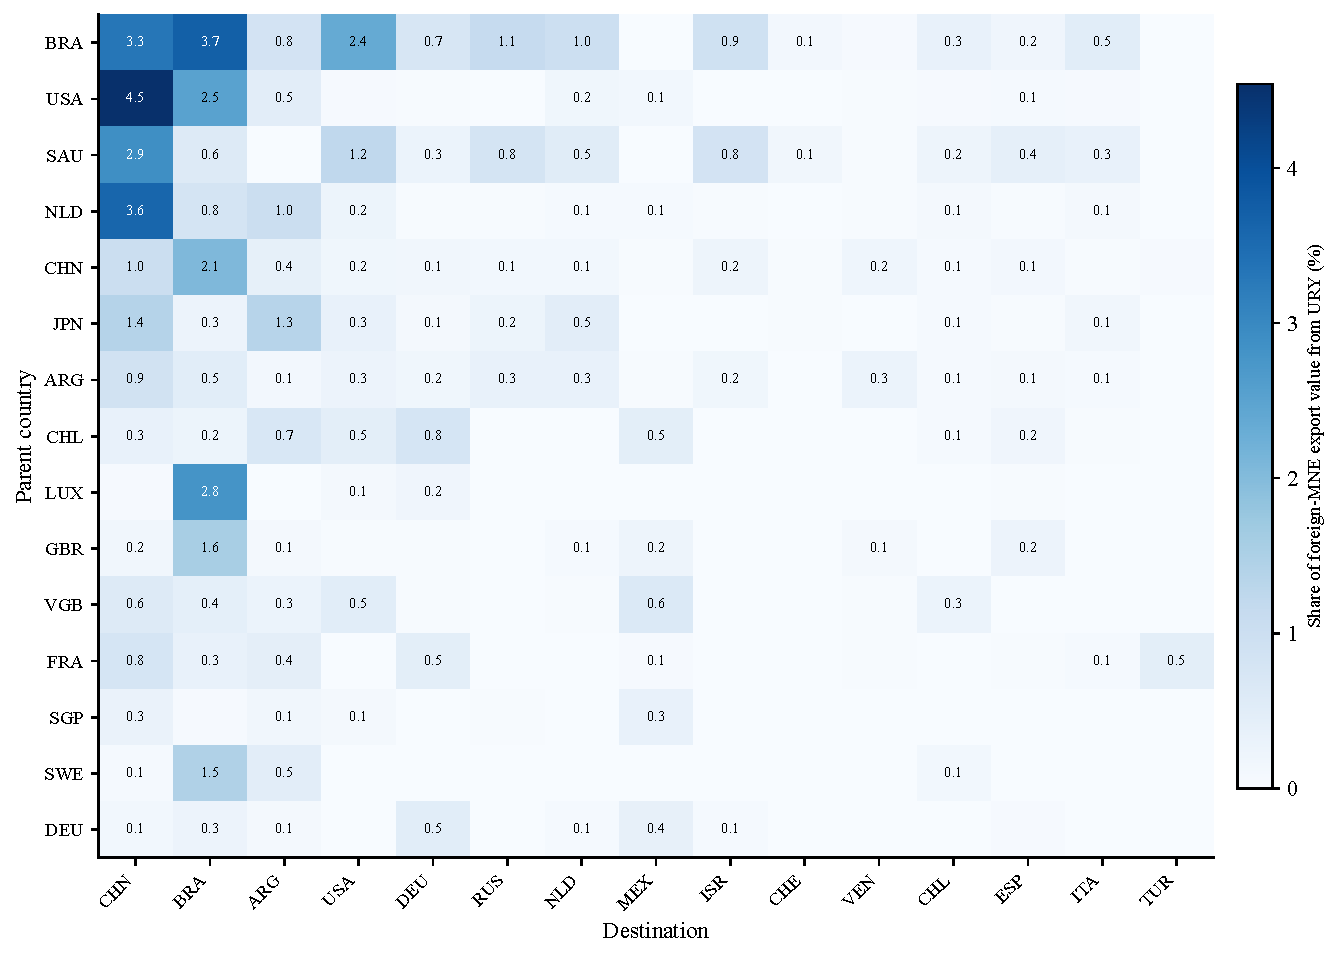
\includegraphics[width=1.0\textwidth,height=0.8\textheight,keepaspectratio]{figures/all/fig_wp1d_heatmap_country_cellpct_URY.pdf}%
  \caption{Uruguay: Foreign-Multinational Exports by Parent Country and Destination}%
  \label{fig:c_hm_URY}%
  \par\vspace{2pt}%
  \parbox{0.92\textwidth}{\footnotesize %
  \textit{Notes:} Percent of the foreign-MNE export value of Uruguay in each parent country and destination pair; fifteen largest parent countries and destinations.\\[3pt]%
  \textit{Source:} Authors' calculations based on customs data matched to Orbis and Dun \& Bradstreet.}%
  \end{figure}
% ---- Figure: Uruguay: Share of Foreign-Multinational Exports Shipped to the Parent Country
\begin{figure}[H]\centering%
  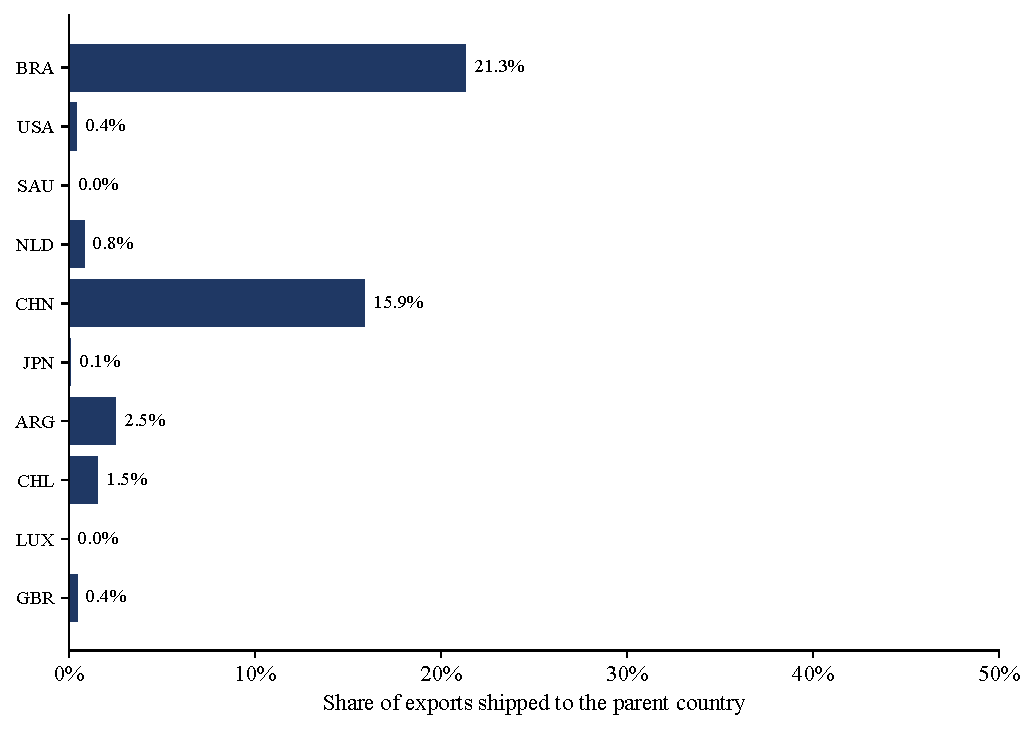
\includegraphics[width=0.85\textwidth,height=0.8\textheight,keepaspectratio]{figures/all/fig_wp1d_home_share_by_parent_URY.pdf}%
  \caption{Uruguay: Share of Foreign-Multinational Exports Shipped to the Parent Country}%
  \label{fig:c_home_URY}%
  \par\vspace{2pt}%
  \parbox{0.92\textwidth}{\footnotesize %
  \textit{Notes:} Percent of each parent country's exports from Uruguay shipped to that same country; ten largest parent countries.\\[3pt]%
  \textit{Source:} Authors' calculations based on customs data matched to Orbis and Dun \& Bradstreet.}%
  \end{figure}
% ---- Table: Uruguay, Agriculture: Multinational Exports by Parent Region and Destination Region
\begin{table}[H]\centering\small%
  \caption{Uruguay, Agriculture: Multinational Exports by Parent Region and Destination Region}%
  \label{tab:c_reg_URY_agro}%
  \adjustbox{max width=\textwidth, max totalheight=0.8\textheight}{\begin{tabular}{lrrrrrrrr}
\toprule
URY: parent region \ destination & Latin America & North America & Europe & Asia & Africa & Oceania & Rest of World & Total \\
\midrule
Latin America & 14.5 & 15.7 & 31.0 & 36.5 & 1.7 & 0.0 & 0.5 & 0.7 \\
North America & 19.5 & 1.4 & 3.9 & 57.8 & 8.9 & 0.0 & 8.6 & 0.3 \\
Europe & 49.7 & 2.3 & 10.8 & 28.2 & 5.8 & 0.0 & 3.2 & 0.6 \\
Asia & 14.1 & 12.9 & 29.8 & 40.9 & 1.6 & 0.0 & 0.7 & 0.6 \\
Africa & 0.1 & 0.1 & 65.5 & 8.3 & 0.8 & 0.1 & 25.2 & 0.0 \\
Oceania & 49.1 & 4.6 & 6.5 & 0.0 & 0.0 & 39.8 & 0.0 & 0.0 \\
Domestic MNEs & 39.2 & 4.6 & 20.3 & 29.1 & 5.1 & 0.0 & 1.7 & 0.4 \\
Local firms & 33.8 & 4.9 & 23.8 & 27.8 & 7.9 & 0.1 & 1.8 & 1.7 \\
\bottomrule
\end{tabular}
}%
  \par\vspace{3pt}%
  \begin{minipage}{0.95\textwidth}\footnotesize %
  \textit{Notes:} Percent of each group's agricultural exports from Uruguay, by destination region (rows add to 100). Last column: the group's exports. Values are annual averages in US\$ billion.\\[3pt]%
  \textit{Source:} Authors' calculations based on customs data matched to Orbis and Dun \& Bradstreet.%
  \end{minipage}%
  \end{table}
% ---- Table: Uruguay, Manufacturing: Multinational Exports by Parent Region and Destination Region
\begin{table}[H]\centering\small%
  \caption{Uruguay, Manufacturing: Multinational Exports by Parent Region and Destination Region}%
  \label{tab:c_reg_URY_manufacturing}%
  \adjustbox{max width=\textwidth, max totalheight=0.8\textheight}{\begin{tabular}{lrrrrrrrr}
\toprule
URY: parent region \ destination & Latin America & North America & Europe & Asia & Africa & Oceania & Rest of World & Total \\
\midrule
Latin America & 68.6 & 7.0 & 15.2 & 6.7 & 2.1 & 0.0 & 0.4 & 0.5 \\
North America & 95.2 & 2.0 & 1.3 & 0.8 & 0.4 & 0.0 & 0.3 & 0.1 \\
Europe & 50.6 & 9.6 & 24.8 & 12.7 & 1.4 & 0.1 & 0.7 & 0.4 \\
Asia & 68.4 & 1.7 & 2.7 & 25.8 & 1.1 & 0.3 & 0.0 & 0.2 \\
Africa & 17.3 & 24.5 & 22.2 & 35.8 & 0.0 & 0.0 & 0.1 & 0.0 \\
Oceania & 99.6 & 0.0 & 0.4 & 0.0 & 0.0 & 0.0 & 0.0 & 0.0 \\
Rest of World & 99.5 & 0.0 & 0.5 & 0.0 & 0.0 & 0.0 & 0.0 & 0.0 \\
Domestic MNEs & 82.4 & 4.1 & 8.8 & 3.0 & 1.7 & 0.0 & 0.0 & 0.3 \\
Local firms & 43.5 & 5.8 & 19.4 & 24.1 & 6.7 & 0.1 & 0.4 & 0.8 \\
\bottomrule
\end{tabular}
}%
  \par\vspace{3pt}%
  \begin{minipage}{0.95\textwidth}\footnotesize %
  \textit{Notes:} Percent of each group's manufacturing exports from Uruguay, by destination region (rows add to 100). Last column: the group's exports. Values are annual averages in US\$ billion.\\[3pt]%
  \textit{Source:} Authors' calculations based on customs data matched to Orbis and Dun \& Bradstreet.%
  \end{minipage}%
  \end{table}
% ---- Table: Uruguay, Mining and Fuels: Multinational Exports by Parent Region and Destination Region
\begin{table}[H]\centering\small%
  \caption{Uruguay, Mining and Fuels: Multinational Exports by Parent Region and Destination Region}%
  \label{tab:c_reg_URY_mining}%
  \adjustbox{max width=\textwidth, max totalheight=0.8\textheight}{\begin{tabular}{lrrrrrrrr}
\toprule
URY: parent region \ destination & Latin America & North America & Europe & Asia & Africa & Oceania & Rest of World & Total \\
\midrule
Latin America & 98.7 & 0.0 & 1.1 & 0.0 & 0.0 & 0.0 & 0.2 & 0.0 \\
North America & 0.0 & 0.7 & 99.1 & 0.0 & 0.2 & 0.0 & 0.0 & 0.1 \\
Europe & 16.2 & 8.9 & 10.8 & 59.6 & 0.1 & 0.0 & 4.5 & 0.0 \\
Asia & 5.3 & 0.0 & 0.0 & 94.7 & 0.0 & 0.0 & 0.0 & 0.0 \\
Africa & 0.0 & 99.0 & 1.0 & 0.0 & 0.0 & 0.0 & 0.0 & 0.0 \\
Oceania & 0.0 & 100.0 & 0.0 & 0.0 & 0.0 & 0.0 & 0.0 & 0.0 \\
Domestic MNEs & 43.3 & 16.7 & 0.0 & 39.6 & 0.0 & 0.0 & 0.4 & 0.0 \\
Local firms & 83.9 & 5.4 & 1.1 & 9.5 & 0.0 & 0.1 & 0.0 & 0.1 \\
\bottomrule
\end{tabular}
}%
  \par\vspace{3pt}%
  \begin{minipage}{0.95\textwidth}\footnotesize %
  \textit{Notes:} Percent of each group's mining and fuels exports from Uruguay, by destination region (rows add to 100). Last column: the group's exports. Values are annual averages in US\$ billion.\\[3pt]%
  \textit{Source:} Authors' calculations based on customs data matched to Orbis and Dun \& Bradstreet.%
  \end{minipage}%
  \end{table}

\subsection{Products}
% ---- Table: Uruguay: Fifteen Largest Export Products
\begin{table}[H]\centering\footnotesize%
  \caption{Uruguay: Fifteen Largest Export Products}%
  \label{tab:c_hs6_URY}%
  \adjustbox{max width=\textwidth, max totalheight=0.8\textheight}{\begin{tabular}{@{}l p{6.4cm} r r r r l@{}}
\toprule
HS6 & Description & US\$bn/yr & Foreign (\%) & Domestic (\%) & Local (\%) & Leading parent \\
\midrule
120100 & Soya beans, whether/\allowbreak{}not broken & 0.79 & 56 & 2 & 43 & USA (0.51) \\
020230 & Meat of bovine animals, frozen, boneless & 0.69 & 67 & 8 & 26 & BRA (0.40) \\
100630 & Semi-milled/\allowbreak{}wholly milled rice, whether/\allowbreak{}not polished/\allowbreak{}glazed & 0.35 & 39 & 53 & 8 & CHN (0.51) \\
202300 & HS 202300 (no description available) & 0.31 & 68 & 7 & 25 & BRA (0.37) \\
020130 & Meat of bovine animals, fresh/\allowbreak{}chilled, boneless & 0.24 & 62 & 10 & 28 & BRA (0.40) \\
040221 & Milk in powder/\allowbreak{}granules/\allowbreak{}other solid form, unsweetened, fat content by weight >1.5\% & 0.20 & 7 & 0 & 93 & PER (0.51) \\
110710 & Malt, not roasted & 0.16 & 100 & 0 & 0 & LUX (0.73) \\
100190 & Wheat other than durum wheat; meslin & 0.13 & 49 & 3 & 48 & USA (0.60) \\
510529 & Wool tops and other combed wool other than combed wool in fragments & 0.13 & 67 & 0 & 33 & FRA (0.64) \\
392330 & Carboys, bottles, flasks and similar articles, of plastics & 0.13 & 23 & 76 & 1 & BRA (1.00) \\
040690 & Cheese (excl. of 0406.10-0406.40) & 0.12 & 24 & 0 & 76 & ALB (0.65) \\
402211 & HS 402211 (no description available) & 0.11 & 7 & 0 & 93 & ARG (0.58) \\
201300 & HS 201300 (no description available) & 0.11 & 60 & 13 & 27 & BRA (0.44) \\
410441 & Tanned/\allowbreak{}crust hides and skins of bovine (incl. buffalo)/\allowbreak{}equine animals, without hair on, in the... & 0.09 & 93 & 0 & 7 & SGP (0.58) \\
440122 & Wood, in chips/\allowbreak{}particles, non-coniferous & 0.09 & 15 & 21 & 63 & GBR (0.64) \\
\bottomrule
\end{tabular}
}%
  \par\vspace{3pt}%
  \begin{minipage}{0.95\textwidth}\footnotesize %
  \textit{Notes:} Fifteen largest HS6 products exported by Uruguay. Foreign, domestic and local: percent of the product's export value. Leading parent: largest parent country and its share of the product's foreign-MNE exports. Values are annual averages in US\$ billion.\\[3pt]%
  \textit{Source:} Authors' calculations based on customs data matched to Orbis and Dun \& Bradstreet.%
  \end{minipage}%
  \end{table}
% ---- Table: Uruguay, Agriculture: Fifteen Largest Export Products
\begin{table}[H]\centering\footnotesize%
  \caption{Uruguay, Agriculture: Fifteen Largest Export Products}%
  \label{tab:c_hs6_URY_agro}%
  \adjustbox{max width=\textwidth, max totalheight=0.8\textheight}{\begin{tabular}{@{}l p{6.4cm} r r r r l@{}}
\toprule
HS6 & Description & US\$bn/yr & Foreign (\%) & Domestic (\%) & Local (\%) & Leading parent \\
\midrule
120100 & Soya beans, whether/\allowbreak{}not broken & 0.79 & 56 & 2 & 43 & USA (0.51) \\
020230 & Meat of bovine animals, frozen, boneless & 0.69 & 67 & 8 & 26 & BRA (0.40) \\
100630 & Semi-milled/\allowbreak{}wholly milled rice, whether/\allowbreak{}not polished/\allowbreak{}glazed & 0.35 & 39 & 53 & 8 & CHN (0.51) \\
202300 & HS 202300 (no description available) & 0.31 & 68 & 7 & 25 & BRA (0.37) \\
020130 & Meat of bovine animals, fresh/\allowbreak{}chilled, boneless & 0.24 & 62 & 10 & 28 & BRA (0.40) \\
040221 & Milk in powder/\allowbreak{}granules/\allowbreak{}other solid form, unsweetened, fat content by weight >1.5\% & 0.20 & 7 & 0 & 93 & PER (0.51) \\
110710 & Malt, not roasted & 0.16 & 100 & 0 & 0 & LUX (0.73) \\
100190 & Wheat other than durum wheat; meslin & 0.13 & 49 & 3 & 48 & USA (0.60) \\
040690 & Cheese (excl. of 0406.10-0406.40) & 0.12 & 24 & 0 & 76 & ALB (0.65) \\
201300 & HS 201300 (no description available) & 0.11 & 60 & 13 & 27 & BRA (0.44) \\
010290 & Live bovine animals other than pure-bred breeding animals & 0.07 & 35 & 0 & 65 & ROU (0.59) \\
151790 & Edible mixtures/\allowbreak{}preparations of animal/\allowbreak{}vegetable fats/\allowbreak{}oils/\allowbreak{}fractions of different fats/\allowbreak{}oils of... & 0.07 & 100 & 0 & 0 & SWE (1.00) \\
102299 & HS 102299 (no description available) & 0.07 & 44 & 0 & 56 & ROU (0.66) \\
040210 & Milk in powder/\allowbreak{}granules/\allowbreak{}other solid form, fat content by weight not >1.5\% & 0.06 & 7 & 0 & 93 & PER (0.96) \\
040510 & Butter & 0.05 & 16 & 0 & 84 & PER (0.93) \\
\bottomrule
\end{tabular}
}%
  \par\vspace{3pt}%
  \begin{minipage}{0.95\textwidth}\footnotesize %
  \textit{Notes:} Fifteen largest agricultural HS6 products exported by Uruguay. Foreign, domestic and local: percent of the product's export value. Leading parent: largest parent country and its share of the product's foreign-MNE exports. Values are annual averages in US\$ billion.\\[3pt]%
  \textit{Source:} Authors' calculations based on customs data matched to Orbis and Dun \& Bradstreet.%
  \end{minipage}%
  \end{table}
% ---- Table: Uruguay, Manufacturing: Fifteen Largest Export Products
\begin{table}[H]\centering\footnotesize%
  \caption{Uruguay, Manufacturing: Fifteen Largest Export Products}%
  \label{tab:c_hs6_URY_manufacturing}%
  \adjustbox{max width=\textwidth, max totalheight=0.8\textheight}{\begin{tabular}{@{}l p{6.4cm} r r r r l@{}}
\toprule
HS6 & Description & US\$bn/yr & Foreign (\%) & Domestic (\%) & Local (\%) & Leading parent \\
\midrule
510529 & Wool tops and other combed wool other than combed wool in fragments & 0.13 & 67 & 0 & 33 & FRA (0.64) \\
392330 & Carboys, bottles, flasks and similar articles, of plastics & 0.13 & 23 & 76 & 1 & BRA (1.00) \\
402211 & HS 402211 (no description available) & 0.11 & 7 & 0 & 93 & ARG (0.58) \\
410441 & Tanned/\allowbreak{}crust hides and skins of bovine (incl. buffalo)/\allowbreak{}equine animals, without hair on, in the... & 0.09 & 93 & 0 & 7 & SGP (0.58) \\
440122 & Wood, in chips/\allowbreak{}particles, non-coniferous & 0.09 & 15 & 21 & 63 & GBR (0.64) \\
940190 & Parts of the seats of 94.01 & 0.07 & 100 & 0 & 0 & CHL (0.32) \\
400510 & Compounded rubber, compounded with carbon black/\allowbreak{}silica, unvulcanised, in primary forms/\allowbreak{}in plat... & 0.06 & 28 & 0 & 72 & ESP (0.99) \\
340211 & Anionic surface-active agents, whether/\allowbreak{}not PURS & 0.06 & 99 & 0 & 1 & BRA (0.84) \\
410792 & Leather further prepared after tanning/\allowbreak{}crusting, incl. parchment-dressed leather, of bovine (i... & 0.06 & 100 & 0 & 0 & SGP (0.56) \\
870421 & Motor vehicles for the transportof goods (excl. of 8704.10), with C-I internal combustion pist... & 0.05 & 73 & 0 & 27 & BRA (1.00) \\
730640 & Tubes, pipes and hollow profiles (excl. of 7306.10-7306.30), welded, of circular cross-section... & 0.05 & 10 & 90 & 0 & DEU (1.00) \\
870323 & Vehicles (excl. of 87.02 and 8703.10) principally designed for the transportof persons, with s... & 0.05 & 97 & 0 & 3 & CHN (0.97) \\
410712 & Leather further prepared after tanning/\allowbreak{}crusting, incl. parchment-dressed leather, of bovine (i... & 0.05 & 87 & 0 & 13 & CHL (0.91) \\
380892 & Fungicides, put up in forms/\allowbreak{}packings for retail sale/\allowbreak{}as preparations/\allowbreak{}articles  & 0.05 & 77 & 18 & 6 & USA (0.99) \\
510111 & Wool, not carded/\allowbreak{}combed, greasy, incl. fleece-washed wool, shorn & 0.04 & 37 & 0 & 63 & PAN (0.52) \\
\bottomrule
\end{tabular}
}%
  \par\vspace{3pt}%
  \begin{minipage}{0.95\textwidth}\footnotesize %
  \textit{Notes:} Fifteen largest manufacturing HS6 products exported by Uruguay. Foreign, domestic and local: percent of the product's export value. Leading parent: largest parent country and its share of the product's foreign-MNE exports. Values are annual averages in US\$ billion.\\[3pt]%
  \textit{Source:} Authors' calculations based on customs data matched to Orbis and Dun \& Bradstreet.%
  \end{minipage}%
  \end{table}
% ---- Table: Uruguay, Mining and Fuels: Fifteen Largest Export Products
\begin{table}[H]\centering\footnotesize%
  \caption{Uruguay, Mining and Fuels: Fifteen Largest Export Products}%
  \label{tab:c_hs6_URY_mining}%
  \adjustbox{max width=\textwidth, max totalheight=0.8\textheight}{\begin{tabular}{@{}l p{6.4cm} r r r r l@{}}
\toprule
HS6 & Description & US\$bn/yr & Foreign (\%) & Domestic (\%) & Local (\%) & Leading parent \\
\midrule
710812 & Gold (incl. gold plated with platinum), in unwrought forms (excl. powder) & 0.06 & 100 & 0 & 0 & CAN (1.00) \\
271600 & Electrical energy (optional heading) & 0.04 & 0 & 0 & 100 & CHL (1.00) \\
271011 & Light petroleum oils and preparations & 0.03 & 0 & 0 & 100 & DEU (1.00) \\
710310 & Precious stones (excl. diamonds) and semi-precious stones, unworked/\allowbreak{}simply sawn/\allowbreak{}roughly shaped... & 0.01 & 28 & 0 & 72 & BGR (0.44) \\
252329 & Portland cement (excl. white cement, whether/\allowbreak{}not artificially coloured), whether/\allowbreak{}not coloured & 0.01 & 92 & 0 & 8 & BRA (1.00) \\
252210 & Quicklime & 0.01 & 0 & 0 & 100 & -- \\
710399 & Precious stones (excl. diamonds, rubies, saphires and emeralds) and semi-precious stones, whet... & 0.00 & 5 & 0 & 95 & BGR (0.99) \\
271019 & Petroleum oils and oils obtained from bituminous minerals (other than crude) and preparations ... & 0.00 & 2 & 0 & 98 & USA (0.76) \\
251612 & Granite, merely cut, by sawing/\allowbreak{}othw., into blocks/\allowbreak{}slabs of a rectangular (incl. square) shape & 0.00 & 72 & 0 & 28 & CZE (0.99) \\
271112 & Propane, liquefied & 0.00 & 0 & 0 & 100 & -- \\
711620 & Articles of precious/\allowbreak{}semi-precious stones (natural/\allowbreak{}synthetic/\allowbreak{}reconstructed) & 0.00 & 46 & 0 & 54 & BGR (1.00) \\
711319 & Articles of jewellery and parts thereof , of other precious metal (excl. silver), whether/\allowbreak{}not ... & 0.00 & 98 & 0 & 2 & DZA (1.00) \\
250810 & Bentonite & 0.00 & 0 & 0 & 100 & -- \\
711299 & Waste and scrap of precious metal/\allowbreak{}of metal clad with precious metal; other waste and scrap con... & 0.00 & 100 & 0 & 0 & DEU (0.73) \\
262030 & Ash and residues (excl. from the manufacture of iron/\allowbreak{}steel) containing mainly copper & 0.00 & 100 & 0 & 0 & DEU (1.00) \\
\bottomrule
\end{tabular}
}%
  \par\vspace{3pt}%
  \begin{minipage}{0.95\textwidth}\footnotesize %
  \textit{Notes:} Fifteen largest mining and fuels HS6 products exported by Uruguay. Foreign, domestic and local: percent of the product's export value. Leading parent: largest parent country and its share of the product's foreign-MNE exports. Values are annual averages in US\$ billion.\\[3pt]%
  \textit{Source:} Authors' calculations based on customs data matched to Orbis and Dun \& Bradstreet.%
  \end{minipage}%
  \end{table}
\end{document}
